\documentclass[11pt,a4paper]{article}
% allow both latex and PDFlatex compatibility  (from pdfTeX FAQ)
\usepackage{hyperlatex}
\usepackage{pifont}
\usepackage{amsmath}
\usepackage{amssymb}
\usepackage[english]{babel}
\usepackage{alltt}
\usepackage{color}
\texonly{
\newif\ifpdf
\ifx\pdfoutput\undefined
    \pdffalse% we are not running PDFLaTeX
\else\pdfoutput=1% we are running PDFLaTeX
\pdftrue
\fi
\ifpdf
  \usepackage[pdftex]{graphicx}
  \usepackage{soul}% hilighting
  \pdfcompresslevel=9
\else
  \usepackage{graphicx}
\fi
\usepackage{xspace} % insere un espace si necessaire 
\ifpdf
  \usepackage[pdftex,pageanchor=true,hyperindex=true,pagebackref=true,pdfhighlight=/O,
colorlinks=true,pdfauthor={Julien Pommier},urlcolor=blue]{hyperref}
\else
  \usepackage[dvips,pageanchor=true,hyperindex=true,pagebackref=true,pdfhighlight=/O,
colorlinks=true,pdfauthor={Julien Pommier},urlcolor=blue]{hyperref}
\fi
\usepackage{makeidx}
\usepackage{underscore}
\oddsidemargin -0.9cm
\evensidemargin -0.9cm
\topmargin -1cm
\textheight 22.5cm
\textwidth 17.6cm
\headheight 1.0cm
}% end texonly



\W \newcommand{\HlxIcons}{./}
%\W \usepackage{frames} % navigation panel
\W \htmldirectory{gfm}
\W \htmlname{gfm}
%\W \HlxFramesNavigation


\makeindex
\definecolor{darkblue}{rgb}{0.,0.,0.4}
\definecolor{darkgreen}{rgb}{0.,0.4,0.}
\definecolor{darkyel}{rgb}{0.3,0.3,0.}
\definecolor{darkred}{rgb}{0.3,0.,0.}
\definecolor{lightred}{rgb}{1,0.5,0.5}
\definecolor{red}{rgb}{1.0,0.,0.}
\definecolor{gray80}{rgb}{0.2,0.2,0.2}
\definecolor{darkmag}{rgb}{0.2,0.0,0.4}
\definecolor{sepbg}{rgb}{1,1,0.7} % see also hilighted in docstyle.css

\htmlonly{
%  \htmlpanelfield{Contents}{gfmcontents}
  \htmlpanelfield{Index}{gfmindex}
  \htmlcss{docstyle.css}
%\htmlcss{gfm.css}

\setcounter{htmldepth}{3}%only section && subsection are given their own node

  \newcommand{\hypertarget}[1]{\label{#1}}
  \newcommand{\vfill}{}
  \newcommand{\newpage}{}
  \newcommand{\textrm}[1]{\mathrm{#1}}
  \newcommand{\text}[1]{\mathrm{#1}}
  \newcommand{\sf}[1]{#1}
  \newcommand{\star}{*}
  \newcommand{\WEB}[2]{\xmlattributes*{a}{target="_top"}\xlink{#2}{#1}}
  \newcommand{\nabla}{\htmlsym{nabla}}%renamed \xmlent by lastest version of hyperlatex
  \newcommand{\ell}{\htmlsym{tau}}
  \newcommand{\lambda}{\htmlsym{lambda}}
  \newcommand{\varepsilon}{\htmlsym{epsilon}}
  \newcommand{\phi}{\htmlsym{phi}}
  \newcommand{\varphi}{\htmlsym{phi}}
  \newcommand{\psi}{\htmlsym{psi}}
  \newcommand{\sigma}{\htmlsym{sigma}}
  \newcommand{\nu}{\htmlsym{nu}}
  \newcommand{\beta}{\htmlsym{beta}}
  \newcommand{\gamma}{\htmlsym{gamma}}
  \newcommand{\Gamma}{\htmlsym{Gamma}}
  \newcommand{\Delta}{\htmlsym{Delta}}
  \newcommand{\delta}{\htmlsym{delta}}
  \newcommand{\Omega}{\htmlsym{Omega}}
  \newcommand{\omega}{\htmlsym{omega}}
  \newcommand{\partial}{\htmlsym{part}}
  \newcommand{\sum}{\htmlsym{sum}}
  \newcommand{\int}{{\Large\htmlsym{int}}}
%  \newcommand{\htmlimg}[1]{\htmlimage{#1}}% will be deprecated as soon as debian upgrades
  \newcommand{\kw}[1]{\textcolor{darkblue}{\texttt{#1}}}
  \newcommand{\hlnk}[2]{\link{#1}{#2}}
  \newcommand{\kwl}[2]{\xmlattributes*{a}{class="matlab"}\texttt{\link{#2}{#1}}}
  \newcommand{\vartype}[1]{\xmlattributes*{a}{class="mltype"}{\link{#1}{typelist}}}
  \newenvironment{minipage}[2]{}{}
  \newenvironment{matlab}{\begin{rawxml}<div class="mlabcode">\end{rawxml}\begin{example}}{\end{example}\begin{rawxml}</div>\end{rawxml}}
  \newenvironment{mcode}{\begin{rawxml}<div class="mlabcode">\end{rawxml}\begin{example}}{\end{example}\begin{rawxml}</div>\end{rawxml}}
  \newcommand{\hil}[1]{\begin{rawxml}<span class="hilighted">\end{rawxml}#1\begin{rawxml}</span>\end{rawxml}}
  \newcommand{\sep}[1]{\medskip\par\hil{#1}}
}


\texonly {
  \newcommand{\WEB}[2]{\href{#1}{#2}}
  \newcommand{\kw}[1]{\textcolor{darkblue}{\texttt{#1}}}
  \newcommand{\hlnk}[2]{\hyperlink{#1}{\textcolor{darkblue}{#2}}}
  \newcommand{\kwl}[2]{\texttt{\hyperlink{#1}{\textcolor{darkblue}{#2}}}}
  \newcommand{\vartype}[1]{\texttt{\textit{\hyperlink{typelist}{\textcolor{darkred}{#1}}}}}
  \newenvironment{matlab}{\begin{alltt}}{\end{alltt}}
  \newenvironment{mcode}{\begin{alltt}}{\end{alltt}}
  \newcommand{\hil}[1]{\colorbox{sepbg}{#1}}
  \newcommand{\sep}[1]{\medskip\par#1}
}



% some commands used by the perl script
\newcommand{\mlabprompt}{\texttt{\textcolor{gray80}{>>}}}
\T \newcommand{\mlabcomment}[1]{\textrm{\textcolor{gray80}{#1}}}
\W \newcommand{\mlabcomment}[1]{\textcolor{gray80}{#1}}
\newcommand{\mlabkeyword}[1]{\textcolor{darkmag}{#1}}
\T \newcommand{\mlaboutput}[1]{\textsl{#1}}
\W \newcommand{\mlaboutput}[1]{\textcolor{darkmag}{#1}}
\newcommand{\inlinematlab}[1]{\texttt{#1}}
\newcommand{\str}[1]{'\textcolor{darkgreen}{\texttt{#1}}'}
\newcommand{\mesh}{mesh\xspace}
\newcommand{\mf}{mesh fem\xspace}
\newcommand{\mim}{mesh im\xspace}
\newcommand{\mdbrick}{mdbrick\xspace}
\newcommand{\mdstate}{mdstate\xspace}
\newcommand{\model}{model\xspace}
\newcommand{\slc}{mesh slice\xspace}
\newcommand{\spmat}{sparse matrix\xspace}
\newcommand{\precond}{preconditioner\xspace}
\newcommand{\fem}{fem\xspace}
\newcommand{\gt}{geotrans\xspace}
\newcommand{\integ}{integ\xspace}
\newcommand{\cvstruct}{cvstruct\xspace}
\newcommand{\tint}{\vartype{int}\xspace}
\newcommand{\tuint}{\vartype{uint32}\xspace}
\newcommand{\thobj}{\vartype{hobj}\xspace}
\newcommand{\tscal}{\vartype{scalar}\xspace}
\newcommand{\tvec}{\vartype{vec}\xspace}
\newcommand{\tivec}{\vartype{ivec}\xspace}
\newcommand{\tmesh}{\vartype{mesh}\xspace}
\newcommand{\tcmesh}{\vartype{const\_mesh}\xspace}
\newcommand{\tcvstruct}{\vartype{cvstruct}\xspace}
\newcommand{\tgeotrans}{\vartype{geotrans}\xspace}
\newcommand{\tmf}{\vartype{mesh\_fem}\xspace}
\newcommand{\tmim}{\vartype{mesh\_im}\xspace}
\newcommand{\tmdstate}{\vartype{mdstate}\xspace}
\newcommand{\tmodel}{\vartype{model}\xspace}
\newcommand{\tmdbrick}{\vartype{mdbrick}\xspace}
\newcommand{\tslc}{\vartype{mesh\_slice}\xspace}
\newcommand{\tfem}{\vartype{fem}\xspace}
\newcommand{\teltm}{\vartype{eltm}\xspace}
\newcommand{\tinteg}{\vartype{integ}\xspace}
\newcommand{\timat}{\vartype{imat}\xspace}
\newcommand{\tmat}{\vartype{mat}\xspace}
\newcommand{\tspmat}{\vartype{spmat}\xspace}
\newcommand{\tprecond}{\vartype{precond}\xspace}
\newcommand{\tstr}{\vartype{string}\xspace}
\texonly{
  \newcommand{\Mlab}{{\sf Matlab\raisebox{4pt}{\tiny {\textregistered}}}\xspace}
}\htmlonly {
  \newcommand{\Mlab}{Matlab\xspace}  
}
\newcommand{\mlab}{{\sf matlab}\xspace}
\newcommand{\pdetool}{{\sf pdetool}\xspace}
\newcommand{\gf}{{\sf getfem${++}$}\xspace}
\newcommand{\Gf}{{\sf Getfem${++}$}\xspace}
\newcommand{\gfi}{{\sf getfem-interface}\xspace}
\newcommand{\Gfi}{{\sf Getfem-interface}\xspace}
\newcommand{\gfm}{{\sf getfem-matlab}\xspace}
\newcommand{\Gfm}{{\sf Getfem-matlab}\xspace}
\newcommand{\SuperLU}{\WEB{http://crd.lbl.gov/\~{}xiaoye/SuperLU/}{SuperLU}\xspace}
\newcommand{\VTK}{\WEB{http://www.vtk.org}{VTK}\xspace}
\newcommand{\OpenDX}{\WEB{http://www.opendx.org}{OpenDX}\xspace}
\T \newenvironment{purpose}{\begin{flushleft}\textsc{\large Purpose:\\\vskip.1truecm}}{\end{flushleft}}
\W \newenvironment{purpose}{\begin{rawxml}<div class="mlpurp"><h3>Purpose</h3><div class="mlbox">\end{rawxml}}{\begin{rawxml}</div></div>\end{rawxml}}
\T \newenvironment{synopsis}{\begin{flushleft}\textsc{\large Synopsis:}\begin{alltt}}{\end{alltt}\end{flushleft}}
\W \newenvironment{synopsis}{\begin{rawxml}<div class="mlsynopsis"><h3>Synopsis</h3><div class="mlbox">\end{rawxml}\begin{example}}{\end{example}\begin{rawxml}</div></div>\end{rawxml}}
\T \newenvironment{cmddescription}{\noindent\textsc{\large Description:\\\vskip.1truecm}}{\par\medskip}
\W \newenvironment{cmddescription}{\begin{rawxml}<div class="mldesc"><h3>Description</h3><div class="mlbox">\end{rawxml}}{\begin{rawxml}</div></div>\end{rawxml}}
\T \newenvironment{cmdexamples}{\noindent\textsc{\large Examples:\\\vskip.1truecm}}{\par\medskip}
\W \newenvironment{cmdexamples}{\begin{rawxml}<div class="mlexamples"><h3>Examples</h3><div class="mlbox">\end{rawxml}}{\begin{rawxml}</div></div>\end{rawxml}}
\T \newenvironment{gfseealso}{\begin{flushleft}\textsc{\large See also:\\\vskip.1truecm}}{\end{flushleft}}
\W \newenvironment{gfseealso}{\begin{rawxml}<div class="mlseealso"><h3>See Also</h3><div class="mlbox">\end{rawxml}}{\begin{rawxml}</div></div>\end{rawxml}}
\newcommand{\warning}[1]{\textcolor{red}{warning} \textit{#1}}
\T \newcommand{\Div}{\textrm{div}}
\W \newcommand{\Div}{div}
\T \newcommand{\Grad}{\textrm{grad}}
\W \newcommand{\Grad}{grad}
\T \newcommand{\Rot}{\textrm{curl}}
\W \newcommand{\Rot}{curl}
\W \newcommand{\to}{\texttt{->}}
\W \newcommand{\vec}[1]{#1}
%\DeclareMathOperator{\Div}{div}
%\DeclareMathOperator{\Rot}{curl}
%\DeclareMathOperator{\Grad}{grad}

\newcommand{\NEW}{\textcolor{lightred}{\textbf{(New in getfem 2.0)}}}

\begin{document}
\htmltitle{Getfem-Matlab Interface}
\htmlpanel{0}%disable navigation panel


\begin{center}
  \texonly{
\includegraphics[width=10cm,angle=0]{logogetfemwhitebg}\\[0.2cm]
  a Generic Finite Element library in C++ \\[0.5cm]
  \fbox{\Huge \sc Matlab\raisebox{4pt}{\tiny {\textregistered}} Interface - User Documentation} \\[0.5cm]
  { \large Yves {\sc Renard}, Julien {\sc Pommier} \footnote{ \it MIP, INSAT, Complexe scientifique de Rangueil, 31077 Toulouse, France, Yves.Renard@insa-toulouse.fr, Julien.Pommier@insa-toulouse.fr } } \\[1.0cm]
  February, 2006\\[1.0cm]
}\htmlonly{
  \xlink{\htmlimg{logogetfem.png}{the getfem logo}}{http://www-gmm.insa-toulouse.fr/getfem}\\
  a Generic Finite Element library in C++ \\
  {\Huge Matlab Interface - User Documentation} \\
  { \large \xlink{Yves Renard}{mailto:Yves.Renard@insa-toulouse.fr}, \xlink{Julien Pommier}{mailto:Julien.Pommier@insa-toulouse.fr}}\\
  { \it MIP, INSAT, Complexe scientifique de Rangueil, 31077 Toulouse, France.}\par
  \today\par\par
}
\end{center}

% \begin{abstract}
% Basic user documentation for GETFEM++.
% \end{abstract}


%%%%%%%%%%%%%%%%%%%%%%%%%%%%%%%%%%%%%%%%%%%%%%%%%%%%%%%%%%%%%%%%%%%%%%%%%
%          INTRODUCTION                                                 %
%%%%%%%%%%%%%%%%%%%%%%%%%%%%%%%%%%%%%%%%%%%%%%%%%%%%%%%%%%%%%%%%%%%%%%%%%

\section*{Introduction}
This guide provides a reference about the \Mlab interface of \gf.  For
a complete reference of \gf, please report to the
\WEB{http://www-gmm.insa-toulouse.fr/getfem/doc}{specific guides},
but you should be able to use the \mlab interface without any
particular knowledge of the getfem internals, although a basic
knowledge about Finite Elements is required.


\vfill
\begin{quote}
Copyright (C) 2000-2020 Yves Renard, Julien Pommier.\\
The program GetFEM is free software; you can redistribute it and/or modify
it under the terms of the GNU Lesser General Public License as published by
the Free Software Foundation; either version 3 of the License, or
(at your option) any later version along with the GCC Runtime Library
Exception either version 3.1 or (at your option) any later version.
This program is distributed in the hope that it will be useful,
but WITHOUT ANY WARRANTY; without even the implied warranty of
MERCHANTABILITY or FITNESS FOR A PARTICULAR PURPOSE.  See the
GNU Lesser General Public License for more details.
You should have received a copy of the GNU  Lesser General Public License
along with this program; if not, write to the Free Software Foundation,
Inc., 51 Franklin Street, Fifth Floor, Boston, MA  02110-1301  USA
\end{quote}
\newpage
\tableofcontents
\newpage

\section{Installation}
\index{installation}
The installation of the \gfi toolbox can be somewhat tricky, since it
combines a C++ compiler, libraries and \Mlab interaction\ldots In
case of troubles with a non-GNU compiler, gcc/g++ ($\geq3.0$) should be a
safe solution.

CAUTION: 
\begin{itemize}
  \item you should not use a different compiler than the one that was used for \gf.
  \item you should have built the \gf static library (i.e. do not use \texttt{./configure --disable-static} when building \gf). On linux/x86\_64 platforms, a mandatory option when building \gf and \gfi (and any static library linked to them) is the \texttt{--with-pic} option of their \texttt{./configure} script. 
\end{itemize}

Here we assume that \gf was installed in the directory
\texttt{\textit{gfdest_dir}} (i.e.  you ran \texttt{./configure --prefix=\textit{gfdest_dir}}
before compiling and installing \gf, the default value being
\texttt{/usr/local}).

Unpack the \gfi archive and run the configure script:\\[2mm]

\verb+# gzip -dc getfem-interface-2.0.tar.gz | tar xvf -+

\verb+# cd getfem-interface-2.0+

If you did install \texttt{getfem++}, then running 
\texttt{./configure} or \texttt{./configure --prefix=\textit{gfdest_dir}}
should be sufficient.\\

Nevertheless, if \texttt{\textit{gfdest_dir}/bin} is not in the \texttt{PATH}, then you will 
have to to provide the path to the \texttt{getfem-config} script
with \texttt{--with-getfem-config=/\textit{gfdest_dir}/bin/getfem-config}.

You may also use \texttt{--with-toolbox-dir=\textit{toolbox_dir}} to
change the default toolbox installation directory (\texttt{\$prefix/getfem_toolbox}).
Use \texttt{./configure --help} for more options.\\[2mm]

When the \texttt{configure} is done, you can compile the toolbox (use \texttt{gmake} if your default
\texttt{make} is not the GNU one)

\verb+# make+\\[1mm]

An optional step is \texttt{make check} in order to check the matlab interface (this sets some environment variables and runs the \texttt{check_all.m} script which is the \texttt{tests/matlab} directory of the distribution)

and install it (the libraries will be copied in \texttt{\textit{gfdest_dir}/lib}, while the MEX-File and M-Files 
will be copied in \texttt{\textit{toolbox_dir}})

\verb+# make install+


If you want to use a different compiler than the one chosen
automatically by the \texttt{./configure} script, just specify its
name on the command line: \texttt{./configure CXX=mycompiler.}


%When the library is installed, you may have to set the
%\texttt{LD_LIBRARY_PATH} environment variable to the directory containing the
%\texttt{libgetfem.so} and \texttt{libgetfemint.so}, which is \texttt{\textit{gfdest_dir}/lib}:

%\texttt{export LD\_LIBRARY\_PATH=\textit{gfdest_dir}/lib} (if you use ksh or bash)

The last step is to add the path to the toolbox in the matlab path: 
\begin{itemize}
\item you can set the environment variable \texttt{MATLABPATH} to \texttt{\textit{toolbox_dir}} (\texttt{export MATLABPATH=\textit{toolbox_dir}} for example).
\item you can put @@addpath('\textit{toolbox_dir}')@@ to your \texttt{\$HOME/matlab/startup.m}
\end{itemize}



More specific instructions can be found in the \kw{README$\star$} files of
the distribution.




\section{Preliminary}

This is just a short summary of the terms employed in this manual. If
you are not familiar with finite elements, this should be useful (but
in any case, you should definitively read the
\WEB{http://home.gna.org/getfem/doc.html}{\gf project documentation}).

The \textbf{mesh}\index{mesh} is composed of
\textbf{convexes}\index{convexes}. What we call convexes can be simple
line segments, prisms, tetrahedrons, curved triangles, of even
something which is not convex (in the geometrical sense). They all
have an associated \textbf{reference convex}\index{reference convex}:
for segments, this will be the $[0,1]$ segment, for triangles this
will be the canonical triangle $(0,0)-(0,1)-(1,0)$ etc\ldots All convexes
of the mesh are constructed from the reference convex through a
\textbf{geometric transformation}\index{geometric transformation}. In
simple cases (when the convexes are simplices for example), this
transformation will be linear (hence it is easily inverted, which can
be a great advantage). In order to define the geometric
transformation, one defines \textbf{geometrical
  nodes}\index{geometrical nodes} on the reference convex. The
geometrical transformation maps these nodes to the \textbf{mesh
  nodes}\index{mesh nodes}.

On the mesh, one defines a set a basis functions: the
\textbf{FEM}\index{FEM}. A FEM is associated at each convex. The basis
functions are also attached to some geometrical points (which can be
arbitrarily chosen). These points are similar to the mesh nodes, but
\textbf{they don't have to be the same} (this only happens on very
simple cases, such as a classical P1 fem on a triangular mesh). The
set of all basis functions on the mesh forms the basis of a vector
space, on which the PDE will be solved. These basis functions (and
their associated geometrical point) are the \textbf{degrees of freedom
  (dof)}\index{degrees of freedom}\index{dof}. The FEM is said to be
\textbf{Lagrangian}\index{Lagrangian} when each of its basis functions
is equal to one at its attached geometrical point, and is null at the
geometrical points of others basis functions. This is an important
property as it is very easy to
\textbf{interpolate}\index{interpolation} an arbitrary function on the
finite elements space.

The finite elements method involves evaluation of integrals of these
basis functions (or product of basis functions etc\ldots) on convexes (and
faces of convexes). In simple cases (polynomial basis functions and
linear geometrical transformation), one can evaluate analytically
these integrals. In other cases, one has to approximate it, using
\textbf{quadrature formulas}\index{quadrature formulas}. Hence, at
each convex is attached an \textbf{integration
  method}\index{integration method} along with the FEM.  If you have
to use an approximate integration method, always choose carefully its
order(i.e. highest degree of the polynomials who are exactly
integrated with the method) : the degree of the FEM, of the polynomial
degree of the geometrical transformation, and the nature of the
elementary matrix have to be taken into account. If you are unsure
about the appropriate degree, always prefer a high order integration
method (which will slow down the assembly) to a low order one which
will produce a useless linear-system.

The process of construction of a global linear system from integrals of basis
functions on each convex is the \textbf{assembly}\index{assembly}.

A mesh, with a set of FEM attached to its
convexes is called a \textbf{mesh\_fem} object in Getfem++.

A mesh, with a set of integration methods attached to its
convexes is called a \textbf{mesh\_im} object in Getfem++ \NEW.

A \tmf can be used to approximate scalar fields (heat, pression, ..),
or vector fields (displacement, electric field, ..). A \tmim will be
used to perform numerical integrations on these fields.  Most of the
finite elements implemented in Getfem++ are scalar (however, TR0 and
edges elements are also available). Of course, these scalar FEMs can
be used to approximate each component of a vector field. This is done
by setting the \textbf{Qdim} of the \tmf to the dimension of the
vector field (i.e. Qdim=1 $\Rightarrow$ scalar field, Qdim=2 $\Rightarrow$ 2D vector field
etc\ldots).

When solving a PDE, one often has to use more than one FEM. The most important one will be of course the one on which is defined the solution of the PDE. But most PDEs involve various coefficients, for example:
\begin{equation*}
\nabla.(\lambda(x)\nabla u) = f(x).
\end{equation*}
Hence one has to define a FEM for the main unknown $u$, but also for the data $\lambda(x)$ and $f(x)$ if they are not constant. In order to interpolate easily these coefficients in their finite element space, one often choose a Lagrangian FEM.

The convexes, mesh nodes, and dof are all numbered. We sometimes refer to the
number associated to a convex as its \textit{convex id}\index{convex id} (contracted to
\textit{cvid}\index{cvid}). Mesh node numbers are also called \textit{point id}\index{point id} (contracted
to \textit{pid}\index{pid}). Faces of convexes do not have a global numbering, but only a local number in each convex. Hence functions which need or return a list of faces\index{list of faces} will always use a two-rows matrix, the first one containing convex IDs, and the second one containing local face number.

While the \textbf{dof} are always numbered consecutively, \textbf{this is not always the
  case for point ids and convex ids}, especially if you have removed points or
convexes from the mesh. To ensure that they form a continuous sequence
(starting from 1), you have to call @@gf_mesh_set(m,'optimize structure')@@.

\section{Changes from the \gfi-1.7}

A (small) number of changes have been made which break backward compability with the releases 1.x of gfi. The most important one, is the splitting of the old \mf structure into two parts:
\begin{itemize}
\item \tmf objects, which now hold only the finite elements
\item \tmim objects, which hold the integration methods
\end{itemize}
As a consequence, the assembly routines require a \tmim object.


Another important change is the displacement of the ``boundaries'' from the old \mf objects into the \tmesh objects. They are now often refered to as ``mesh regions'' since they can hold set of convex faces, but also sets of convexes. 


The old @@gf\_solve@@ function is now deprecated, and replaced by the
``model bricks'' of \gf. Since these brick act as a black-box, some
low-level examples have been kept for educational purposes.


The sparse matrices and sparse solvers of getfem are now available in
the \gfi (these where required by the python interface since python
does not have any sparse matrix routines). Note that these solvers
(cg, superlu, etc) are often faster than the matlab ones.

\section{\Gfm organization}
The \gfm toolbox is just a convenient interface to the \gf library: you must
have a working \gf installed on your computer. This toolbox
provides a big \texttt{mex-file}\index{mex} (c++ binary callable from \mlab) and
some additional \texttt{m-files} (documentation and extra-functionalities).
All the functions of \Gfm are prefixed by \kw{gf\_} (hence typing
\kw{gf\_} at the \mlab prompt and then pressing the \kw{<tab>} key is
a quick way to obtain the list of getfem functions).

\subsection{Functions}

\begin{tabular}{|lp{0.7\textwidth}|}
\hline
##gf\_workspace        & workspace management\\
##gf_util              & miscellanous utility functions\\
##gf\_delete              & destroy a \gf object (\mesh , \mf , \mim etc..)\\
##gf_cvstruct_get     & retrieve informations from a \cvstruct object\\
##gf\_geotrans          & define a geometric transformation\\
##gf\_geotrans_get          & retrieve informations from a \gt object\\
##gf\_mesh                   & creates a new \mesh object\\
##gf\_mesh\_get           & retrieve informations from a \mesh object\\
##gf\_mesh\_set           & modify a \mesh object\\
##gf\_eltm                  & define an elementary matrix\\
##gf\_fem                    & define a \fem\\
##gf\_fem_get                    & retrieve informations from a \fem object\\
##gf\_integ             & define a integration method\\
##gf\_integ_get             & retrieve informations from an \integ object\\
##gf\_mesh\_fem          & creates a new \mf object\\
##gf\_mesh\_fem\_get        & retrieve informations from a \mf object\\
##gf\_mesh\_fem\_set       & modify a \mf object\\
##gf\_mesh\_im          & creates a new \mim object \NEW\\
##gf\_mesh\_im\_get        & retrieve informations from a \mim object\\
##gf\_mesh\_im\_set       & modify a \mim object\\
##gf\_slice            & create a new \slc object\\
##gf\_slice\_get        & retrieve informations from a \slc object\\
##gf\_slice\_set        & modify a \slc object\\
##gf\_spmat            & create a \spmat object \NEW\\
##gf\_spmat\_get        & perform computations with the \spmat\\
##gf\_spmat\_set        & modify the \spmat\\
##gf\_precond          & create a \precond object \NEW\\
##gf\_precond\_get      & perform computations with the \precond\\
##gf\_linsolve         & interface to various linear solvers provided by getfem (\SuperLU, conjugated gradient etc.) \NEW\\
##gf\_asm             & assembly routines\\
##gf\_solve           & various solvers for usual PDEs (obsoleted by the \mdbrick objects)\\
##gf\_compute         & computations involving the solution of a PDE (norm, derivative, etc..)\\
##gf\_mdbrick         & create a ``model brick'' \NEW\\
##gf\_mdbrick\_get         & retrieve information from a \mdbrick object.\\
##gf\_mdbrick\_set         & modify a \mdbrick object.\\
##gf\_mdstate         & create a ``model state'' \NEW\\
##gf\_mdstate\_get         & retrieve information from a \mdstate object.\\
##gf\_mdstate\_set         & modify a \mdstate object.\\
##gf\_model           & create a ``model'' object \NEW\\
##gf\_model\_get           & retrieve information from a \model object.\\
##gf\_model\_set           & modify a \model object.\\
##gf\_plot\_mesh        & plotting of mesh\\
##gf\_plot            & plotting of 2D and 3D fields\\
##gf\_plot\_1D          & plotting of 1D fields\\
##gf\_plot\_slice     & plotting of a mesh slice\\
\hline
\end{tabular}


\subsection{Objects}
\begin{figure}
\begin{center}
\T \begin{minipage}[c]{8cm}
\texonly{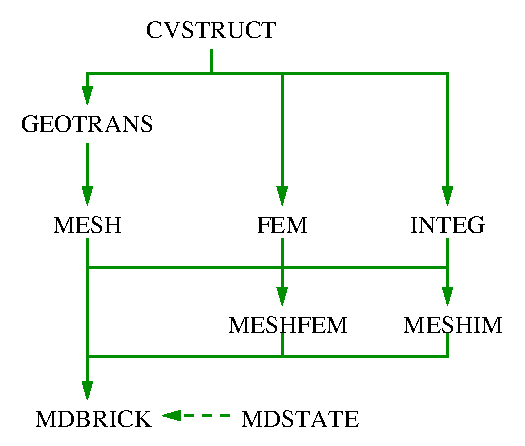
\includegraphics[width=8cm]{hierarchy}}\htmlonly{\htmlimg{hierarchy.png}{objects relations}}
\T \end{minipage}\T \hspace{.3cm}
\end{center}
\T \begin{center}
\T \begin{minipage}[c]{12cm}
  \small
  \textit{GEOTRANS}\index{geometric transformation}: geometric transformations (defines the shape/position of the convexes), created with ##gf\_geotrans\\
  \textit{MESH}\index{mesh}: mesh structure (nodes, convexes, geometric transformations for each convex), created with ##gf\_mesh\\
  \textit{INTEG}\index{integration method}: integration method (exact, quadrature formula\ldots).  Although
  not linked directly to GEOTRANS, an integration method is
  usually specific to a given convex structure. Created with ##gf\_integ \\
  \textit{FEM}\index{FEM}: the finite element method (one per convex, can be PK, QK,
  HERMITE,
  etc\ldots). Created with ##gf\_fem \\
  \textit{CVSTRUCT}\index{convex structure}: stores formal information convex structures (nb. of
  points, nb. of faces which are themselves convex structures).\\
  \textit{MESHFEM}\index{mesh_fem}: object linked to a mesh, where each convex has been
  assigned a FEM. Created with  ##gf\_mesh\_fem.\\
  \textit{MESHIM}\index{mesh_im}: object linked to a mesh, where each convex has been
  assigned an integration method. Created with  ##gf\_mesh\_im.\\
  \textit{MESHSLICE}\index{slice}: object linked to a mesh, very similar to a P1-discontinuous \mf. Used for fast interpolation and plotting.\\
   \textit{MDBRICK}\index{mdbrick}: ``model brick'' , an abstraction of a part of solver (for example, the part which build the tangent matrix, the part which handles the dirichlet conditions, etc.). These objects are stacked to build a complete solver for a wide variety of problems. They typically use a number of \mf, \mim etc.\\
   \textit{MDSTATE}\index{mdstate}: ``model state'', holds the global data for a stack of mdbricks (global tangent matrix, right hand side etc.). 
   \textit{MODEL}\index{model}: ``model'', holds the global data, variables and description of a model. Evolution of ``model state'' object for 4.0 version of \gf.
\T \end{minipage}
\T \end{center}
\caption{\Gfi objects hierarchy}\label{fig:hierarchy}
\end{figure}
Various ``objects'' can be manipulated by the \gfm toolbox, see fig. \ref{fig:hierarchy}. The MESH and MESHFEM objects are the two most important objects. 

The \gfm toolbox uses its own memory management\index{memory management}. Hence \gf objects are
not cleared when a 
\begin{matlab}
>> \kw{clear all}
\end{matlab}
is issued at the \mlab prompt, but
instead the function 
\begin{matlab}
>> gf\_workspace('clear all')
\end{matlab}
should be used. The various \gfm object can be accessed via \textit{handles} (or
\textit{descriptors}), which are just \mlab structures containing 32-bits integer identifiers to
the real objects. Hence the \mlab command 
\begin{matlab}
>> \kw{whos}
\end{matlab}
does not report the memory consumption of \gf objects (except the marginal space
 used by the handle). Instead, you should use
\begin{matlab}
>> gf\_workspace('stats')
\end{matlab}

There are two kinds of \gfm objects:
\begin{itemize}
\item static ones, which can not be deleted: ELTM, FEM, INTEG,
  GEOTRANS and CVSTRUCT. Hopefully their memory consumption is very low.
\item dynamic ones, which can be destroyed, and are handled by the
  \kw{gf\_workspace} function: MESH, MESHFEM, MESHIM, SLICE, SPMAT, PRECOND.
\end{itemize}
The objects MESH and MESHFEM are not independent: a MESHFEM object is
always linked to a MESH object, and a MESH object can be used by
several MESHFEM objects. Hence when you request the destruction of a
MESH object, its destruction might be delayed until it is not used anymore
by any MESHFEM (these objects waiting for deletion are listed in
the \textit{anonymous workspace} section of
@@gf\_workspace('stats')@@).

\section{Examples}
\subsection{A step-by-step basic example}
This example shows the basic usage of getfem, on the {\"u}ber-canonical
problem above all others: solving the Laplacian\index{Laplacian}, $\Delta u+f=0$ on a
square, with the Dirichlet condition $u=g(x)$ on the domain boundary.
\label{laplacianexample}

The first step is to \textbf{create a mesh}. Since \gf does not come with its
own mesher, one has to rely on an external mesher (see
@@gf_mesh('import')@@), or use very simple meshes.  For this example,
we just consider a regular mesh\index{cartesian mesh} whose nodes are
$\{x_{i=0\ldots10,j=0..10}=(i/10,j/10)\}$.
\begin{matlab}
% creation of a simple cartesian mesh
>> m = gf_mesh('cartesian',[0:.1:1],[0:.1:1])
m =
     id: 0
    cid: 0
\end{matlab}
If you try to look at the value of \kw{m}, you'll notice that it appears to be a structure
containing two integers. The first one is its identifier, the second one is its class-id, i.e. an identifier of its type. This small structure is 
just an ``handle'' or ``descriptor'' to the real object, which is
stored in the \gf memory and cannot be represented via \Mlab data
structures. Anyway, you can still inspect the \gf objects via the
command @@gf\_workspace('stats')@@. 

Now we can try to have a \textbf{look at the mesh}, with its vertices numbering
and the convexes numbering:
\begin{matlab}
% we enable vertices and convexes labels
>> gf\_plot\_mesh(m, 'vertices', 'on', 'convexes', 'on');
\end{matlab}
As you can see, the mesh is regular, and the numbering of its nodes and convexes
is also regular (this is guaranteed for cartesian meshes, but do not hope a
similar numbering for the degrees of freedom).

The next step is to \textbf{create a \tmf object}. This one links a mesh with a
set of FEM.
\begin{matlab}
>> mf = gf_mesh_fem(m,1);    % create a \tmf of for a field of dimension 1 (i.e. a scalar field)
>> gf\_mesh\_fem\_set(mf,'fem',gf\_fem('FEM_QK(2,2)'));
\end{matlab}
The first instruction builds a new \tmf object, the second argument specifies
that this object will be used to interpolate scalar fields (since the unknown
is a scalar field). The second instruction assigns the $Q^2$ FEM to every convex (each
basis function is a polynomial of degree 4, remember that $P^k\Rightarrow$ polynomials of degree $k$, while $Q^k\Rightarrow$ polynomials of degree $2k$). As $Q^2$ is a polynomial FEM, you can view the expression of its basis functions on the reference convex:
\begin{matlab}
>> gf_fem_get(gf_fem('FEM_QK(2,2)'), 'poly_str')
ans =
    '1 - 3*x - 3*y + 2*x^2 + 9*x*y + 2*y^2 - 6*x^2*y - 6*x*y^2 + 4*x^2*y^2'
    '4*x - 4*x^2 - 12*x*y + 12*x^2*y + 8*x*y^2 - 8*x^2*y^2'
    '-x + 2*x^2 + 3*x*y - 6*x^2*y - 2*x*y^2 + 4*x^2*y^2'
    '4*y - 12*x*y - 4*y^2 + 8*x^2*y + 12*x*y^2 - 8*x^2*y^2'
    '16*x*y - 16*x^2*y - 16*x*y^2 + 16*x^2*y^2'
    '-4*x*y + 8*x^2*y + 4*x*y^2 - 8*x^2*y^2'
    '-y + 3*x*y + 2*y^2 - 2*x^2*y - 6*x*y^2 + 4*x^2*y^2'
    '-4*x*y + 4*x^2*y + 8*x*y^2 - 8*x^2*y^2'
    'x*y - 2*x^2*y - 2*x*y^2 + 4*x^2*y^2'
\end{matlab}

It is also possible to make use of the ``object oriented'' features of matlab. As you may have noticed, when a class ``foo'' is provided by the \gfi , it is build with the function @@gf_foo@@ , and manipulated with the functions @@gf\_foo\_get@@ and @@gf_foo_set@@. But (with matlab 6.x and better) you may also create the object with the @@gfFoo@@ constructor , and manipulated with the @@get(..)@@ and @@set(..)@@ methods. For example, the previous steps could have been:
\begin{matlab}
>> gfFem('FEM_QK(2,2)')
gfFem object ID=0 dim=2, target_dim=1, nbdof=9,[EQUIV, POLY, LAGR], est.degree=4
 -> FEM_QK(2,2)
>> m=gfMesh('cartesian', 0:.1:1, 0:.1:1)
gfMesh object ID=0 [16512 bytes], dim=2, nbpts=121, nbcvs=100
>> mf=gfMeshFem(m,1)
gfMeshFem object: ID=1 [804 bytes], qdim=1, nbdof=0,
  linked gfMesh object: dim=2, nbpts=121, nbcvs=100
>> set(mf, 'fem', gfFem('FEM_QK(2,2)'))
>> mf
gfMeshFem object: ID=1 [1316 bytes], qdim=1, nbdof=441,
  linked gfMesh object: dim=2, nbpts=121, nbcvs=100
\end{matlab}

Now, in order to perform numerical integrations on @@mf@@, we need to \textbf{build a \tmim object}:
\begin{matlab}
% assign the same integration method on all convexes 
>> mim=gf_mesh_im(m, gf\_integ('IM_EXACT_PARALLELEPIPED(2)'));
\end{matlab}
The integration method will be used to compute the various integrals on each element: here we
choose to perform exact computations (no quadrature formula\index{quadrature formulas}), which is possible
since the geometric transformation of these convexes from the reference convex
is linear (this is true for all simplices, and this is also true for
the parallelepipeds of our regular mesh, but it is not true for general
quadrangles), and the chosen FEM is polynomial. Hence it is possible to
analytically integrate every basis function/product of basis
functions/gradients/etc. There are many alternative FEM methods and
integration methods (see \WEB{http://www-gmm.insa-toulouse.fr/getfem/doc}{the
  description of finite element and integration methods}). 

Note however that in the general case, approximate integration methods
are a better choice than exact integration methods.

Now we have to \textbf{find the ``boundary''\index{boundary} of the domain}, in order to set a \index{Dirichlet}
condition. A mesh object has the ability to store some sets of convexes and convex faces. These sets (called ``regions'') are accessed via an integer \#id:
\begin{matlab}
>> border = gf_mesh_get(m,'outer faces');
>> gf_mesh_set(m, 'region', 42, border); % create the region \#42
>> gf_plot_mesh(m, 'regions', [42]); % the boundary edges appears in red
\end{matlab}
Here we find the faces of the convexes which are on the boundary of
the mesh (i.e. the faces which are not shared by two convexes). \textit{remark:} 
we could have used @@gf_mesh_get(m, 'OuTEr_faCes')@@ , as the
interface is case-insensitive, and whitespaces can be replaced by
underscores. The array \kw{border} has two rows, on the first row is a
convex number, on the second row is a face number (which is local to the
convex, there is no global numbering of faces). Then this set of faces
is assigned to the region number 42\index{boundary number}.

At this point, we just have to stack some model bricks and run the
solver to get the solution! The ``model bricks''\index{mdbrick} are
created with the @@gf\_mdbrick@@ (or @@gfMdBrick@@) constructor. A
model brick is basically an object which modifies a global linear
system (tangent matrix for non-linear problems) and its associated
right hand side.  Typical modifications are insertion of the stiffness
matrix for the problem considered (linear elasticity, laplacian, etc),
handling of a set of contraints, Dirichlet condition, addition of a
source term to the right hand side etc. The global tangent matrix and
its right hand side are stored in a ``model state''\index{mdstate}
structure, created with the @@gf_mdstate@@ constructor.


Let us build a problem with an easy solution: $u=x(x-1)y(y-1)+x^5$,
then we have $\Delta u=2(x^2+y^2)-2(x+y)+20x^3$ (the FEM won't be able to
catch the exact solution since we use a $Q^2$ method).


We start with a ``generic elliptic'' brick, which handles $-div(A\nabla u) = \ldots $ problems, where $A$ can be a scalar field, a matrix field, or an order 4 tensor field. By default, $A=1$.
\begin{matlab}
>> b0=gf_mdbrick('generic elliptic',mim,mf)
\end{matlab}

Each brick embeds a number of parameter fields. In the case of the generic elliptic brick, there is only one parameter field, the $A(x)$ coefficient in $-div(A\nabla u)= \ldots$. It is possible to view the list of parameters of the brick with
\begin{matlab}
>> gf_mdbrick_get(b0, 'param list')
ans =

    'A'
>> gf_mdbrick_get(b0, 'param', 'A')

ans =

     1
\end{matlab}

Next we add a Dirichlet condition on the domain boundary:
\begin{matlab}
>> b1=gf_mdbrick('dirichlet',b0,42,mf,'penalized')
\end{matlab}
Here the number @@42@@ is the region number to which the dirichlet condition is applied. The @@'penalized'@@ says that the Dirichlet condition should be imposed via a penalization technique. Other ways are possible (augmented system, direct elimination). A \mf argument is also required, as the Dirichlet condition $u=r$ is imposed in a weak form
$\int_\Gamma u(x)v(x) = \int_\Gamma r(x)v(x) \forall v$ where $v$ is taken in the space of multipliers given by here by @@mf@@.

By default, the Dirichlet brick imposes $u=0$ on the specified boundary. We change this to $u=(x-.5)^2+(y-.5)^2+x/5-y/3$:
\begin{matlab}
>> R=gf_mesh_fem_get(mf, 'eval', \{'(x-.5).^2 + (y-.5).^2 + x/5 - y/3'\});
>> gf_mdbrick_set(b1, 'param', 'R', mf, R); 
\end{matlab}
\textit{Remark:} the polynomial expression was interpolated on @@mf@@.
It is possible only if @@mf@@ is of Lagrange type. In this first
example we use the same \mf for the unknown and for the data such as
@@R@@, but in the general case, @@mf@@ won't be Lagrangian and another
(Lagrangian) \mf will be used for the description of Dirichlet
conditions, source terms etc.


A ``model state'' variable is created, and the solver is launched:
\begin{matlab}
>> mds=gf_mdstate('real')
>> gf_mdbrick_get(b1, 'solve', mds)
\end{matlab}

The model state now contains the solution (as well as other things, such as the linear system which was solved). It is extracted, a display into a \mlab figure.
\begin{matlab}
>> U=gf_mdstate_get(mds, 'state');
>> gf_plot(mf, U, 'mesh','on');
\end{matlab}

\subsection{Another Laplacian with exact solution}
This is the \texttt{tests/matlab/demo_laplacian.m} example.
\input{demolaplacian.tex}

\subsection{Linear and non-linear elasticity}
This example \index{tripod}\index{linear elasticity} uses a mesh that was generated with
\WEB{http://gid.cimne.upc.es}{GiD}\index{GiD}. The object is meshed with
quadratic tetrahedrons. You can find the \texttt{m-file} of this example under
the name \texttt{demo_tripod.m} in the directory \texttt{tests/matlab} of the
toolbox distribution.

\input{demotripod.tex}

Here is the final figure, displaying the Von Mises stress\index{Von Mises}:

\begin{center}
\texonly{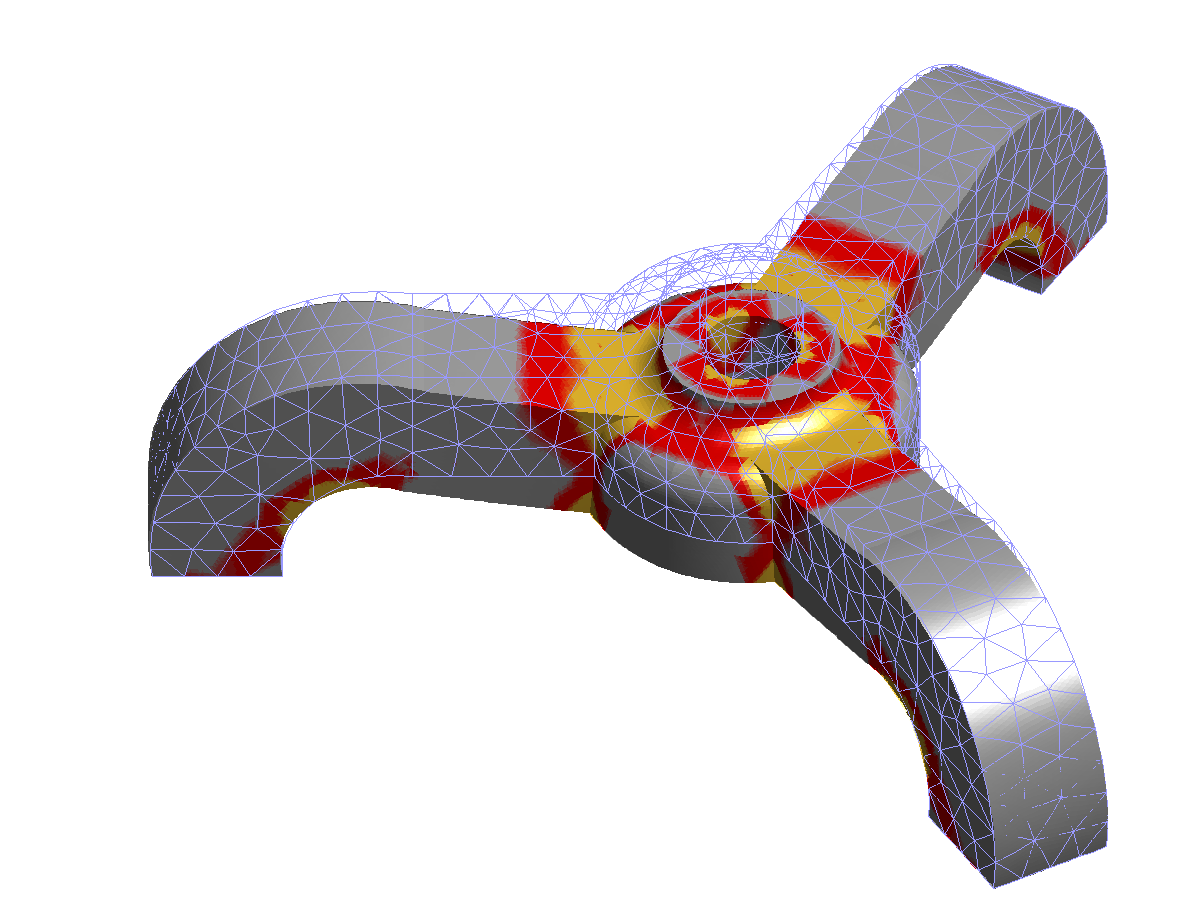
\includegraphics[width=7cm]{tripodvonmiseswithmesh}}\htmlonly{\htmlimg{tripodvonmiseswithmesh_small.png}{deformed tripod}}
\end{center}

\subsection{Avoiding the bricks framework}

The model bricks are very convenient, as they hide most of the details
of the assembly of the final linear systems. However it is also
possible to stay at a lower level, and handle the assembly of linear
systems, and their resolution, directly in \mlab. For example, the
demonstration \texttt{demo\_tripod\_alt.m} is very similar to the
\texttt{demo\_tripod.m} except that the assembly is explicit:

\begin{mcode}
nbd=get(mfd, 'nbdof');
F = gf_asm('boundary_source', 1, mim, mfu, mfd, repmat([0;-10;0],1,nbd));
K = gf_asm('linear_elasticity', mim, mfu, mfd, ...
	   lambda*ones(1,nbd),mu*ones(1,nbd));

% handle Dirichlet condition
[H,R]=gf_asm('dirichlet', 2, mim, mfu, mfd, repmat(eye(3),[1,1,nbd]), zeros(3, nbd));
[N,U0]=gf_spmat_get(H, 'dirichlet_nullspace', R);
KK=N'*K*N;
FF=N'*F;
% solve ...
disp('solving...'); t0 = cputime;
lsolver = 1 % change this to compare the different solvers
if (lsolver == 1),     % conjugate gradient
  P=gfPrecond('ildlt',KK);
  UU=gf_linsolve('cg',KK,FF,P,'noisy','res',1e-9);
elseif (lsolver == 2), % superlu
  UU=gf_linsolve('superlu',KK,FF);
else                   % the matlab "slash" operator 
  UU=KK \verb+\+ FF;
end;
disp(sprintf('linear system solved in \%.2f sec', cputime-t0));
U=(N*UU).'+U0;
\end{mcode}

In \gfi, the assembly of vectors, and matrices is done via the
@@gf\_asm@@ function. The Dirichlet condition $u(x) = r(x)$ is handled
in the weak form $\int (h(x)u(x)).v(x) = \int r(x).v(x)\quad \forall v$ (where
$h(x)$ is a $3\times3$ matrix field -- here it is constant and equal to the
identity). The reduced system @@KK UU = FF@@ is then built via the
elimination of Dirichlet constraints from the original system. Note
that it might be more efficient (and simpler) to deal with Dirichlet
condition via a penalization technique.


\subsection{Other examples}
\begin{itemize}
\item the \kw{demo_refine.m}\index{mesh refinement} script shows a
  simple 2D or 3D bar whose extremity is clamped. An adaptative
  refinement is used to obtain a better approximation in the area
  where the stress is singular (the transition between the clamped
  area and the neumann boundary).

\item the \kw{demo_nonlinear_elasticity.m} script shows a 3D bar which is is bended and twisted. This is a quasi-static problem as the deformation is applied in many steps. At each step, a non-linear (large deformations) elasticity problem is solved.

\item the \kw{demo_stokes_3D_tank.m} script shows a Stokes (viscous fluid) problem in a tank. The \kw{demo_stokes_3D_tank_draw.m} shows how to draw a nice plot of the solution, with mesh slices and stream lines. Note that the \kw{demo_stokes_3D_tank_alt.m} is the old example, which uses the deprecated @@gf_solve@@ function.

\item the \kw{demo_bilaplacian.m} script is just an adaption of the getfem++ example \texttt{tests/bilaplacian.cc}. Solve the bilaplacian (or a Kirchhoff-Love plate model) on a square.

\item the \kw{demo_plasticity.m} script is an adaptation of the getfem++ example \texttt{tests/plasticity.cc}: a 2D or 3D bar is bended in many steps, and the plasticity of the material is taken into account (plastification occurs when the material's Von Mises exceeds a given threshold).

\item the \kw{demo_wave2D.m} is a 2D scalar wave equation example (diffraction of a plane wave by a cylinder), with high order geometric transformations and high order FEMs.
\end{itemize}


\subsection{Using Matlab Object-Oriented features}
The basic functions of the \gfm toolbox do not use any advanced \mlab features
(except that the handles to getfem objects are stored in a small \mlab
structure). But the toolbox comes with a set of \Mlab objects\index{Matlab objects}, which
encapsulate the handles and make them look as real \mlab objects. The aim is
not to provide extra-functionalities, but to have a better integration of the
toolbox with \mlab.

Here is an example of its use:
\begin{matlab}
>> m=gf_mesh('cartesian',0:.1:1,0:.1:1) 
m = 
     id: 0
    cid: 0

>> m2=gfMesh('cartesian',0:.1:1,0:.1:1)
gfMesh object ID=1 [17512 bytes], dim=2, nbpts=121, nbcvs=100
% while \kw{m} is a simple structure, \kw{m2} has been flagged by \mlab
% as  an object of class gfMesh.  Since the \texttt{display} method for 
% these  objects  have  been  overloaded,  the  toolbox  displays  some 
% information about the mesh instead of the content of the structure.
>> gf_mesh_get(m,'nbpts')
ans =
   121
% pseudo member access (which calls ##gf_mesh_get(m2,'nbpts'))
>> m2.nbpts
ans =
   121
\end{matlab}
Refer to the OO-commands reference \ref{OOcommands} for more details.

\section{Command reference}
\subsection{Types}
\hypertarget{typelist}
The expected type of each function argument is indicated in this reference.
Here is a list of these types:
\begin{tabular}{lp{0.7\textwidth}}
  \tint  & integer value \\
  \thobj & a handle\index{handle} for any \gf object.\\
  \tscal & scalar value \\
  \tstr  & string \\
  \tivec & vector of integer values \\
  \tvec  & vector \\
  \timat & matrix of integer values \\
  \tmat  & matrix \\
  \tspmat  & sparse matrix (both matlab native sparse matrices, and getfem sparse matrices)\\
  \tprecond & getfem preconditioner object\\
  \tmesh & mesh object descriptor (or ##gfMesh object)\\
  \tmf   & mesh\_fem object descriptor (or ##gfMeshFem object)\\
  \tmim  & mesh\_im object descriptor( or ##gfMeshIm object)\\
  \tslc  & mesh\_slice object descriptor (or ##gfSlice object)\\
  \tcmesh& non-modifiable mesh object (\tmesh\ and \tmf\ can be used everywhere a \tcmesh\ is required) \\
  \tcvstruct & convex structure descriptor (or ##gfCvStruct object) \\
  \tgeotrans & geometric transformation descriptor (or ##gfGeoTrans object)\\
  \tfem  & fem descriptor (or ##gfFem object)\\
  \teltm & elementary matrix descriptor (or ##gfEltm object)\\
  \tinteg & integration method descriptor (or ##gfInteg object)
\end{tabular}

Arguments listed between square brackets are optional.  Lists
between braces indicate that the argument must match one of the
elements of the list. For example
\begin{mcode}
[X,Y]=dummy(\tint i, \{'foo' | 'bar'\} [,\tvec v])
\end{mcode}
means that the dummy function takes two or three arguments, its first being an integer value, the second a string which is either \str{foo} or \str{bar}, and a third optional argument. It returns two values (with the usual \mlab meaning, i.e.\ the caller can always choose to ignore them).

\newpage
%%%%%%%%%%%%%%%%%%%%%%% GF_WORKSPACE
\subsection{gf\_workspace}
\begin{purpose}
  \hypertarget{gfworkspace}
  \gfm workspace management function\index{memory management}.
\end{purpose}
\begin{synopsis}
@@gf\_workspace('push') 
gf_workspace('pop' [,\thobj i, \thobj j,..])  
gf_workspace('stat') 
gf_workspace('stats')
gf_workspace('keep', \thobj i[,\thobj j, \thobj k..]) 
gf_workspace('clear')
gf_workspace('clear all')
gf_workspace('class name', \thobj i)
@@\end{synopsis}
\begin{cmddescription}
  Getfem uses its own workspaces in \Mlab, independently of the \mlab
  workspaces. The reason for that is the lack of a notion of destructor in
  \mlab. Hence, only descriptors to the real object are manipulated in \mlab\ workspaces, while the real data is managed by \gf functions. The \gf workspaces can be stacked with the commands \str{push}
  and \str{pop}. By default, all getfem variables belong to the root getfem
  workspace. A function can create its own workspace by invoking
  @@gf\_workspace('push')@@ at its beginning. When exiting, this function
  MUST invoke @@gf\_workspace('pop')@@ (you can use \mlab\ exception
  handling to do this cleanly when the function exits on an error, see the
  example below).

  \sep{@@gf\_workspace('push')@@} : create a new temporary workspace on
  the workspace stack.

  
  \sep{@@gf\_workspace('pop' [,i,j,..])@@} : leave the current
  workspace, destroying all getfem variables belonging to it, except
  the one listed after \str{pop}, and the ones which were moved to the
  parent workspace by @@gf\_workspace('keep')@@.

  \sep{@@gf\_workspace('stat')@@} : print informations about variables
  in current workspace.

  \sep{@@gf\_workspace('stats')@@} 
  : print informations about all getfem variables.
  
  \sep{@@gf\_workspace('keep', i[,j,k..])@@}  
  : prevent the listed variables i from being deleted when the command
  @@gf\_workspace('pop')@@ will be called. This is accomplished by
  moving this variable in the parent workspace.

  \sep{@@gf\_workspace('clear')@@}
  : clear the current workspace.

  \sep{@@gf\_workspace('clear all')@@}
  : clear every workspace, and return to the main workspace.

  \sep{@@gf\_workspace('class name', i)@@}
  : return the class name of object @@i@@ (if @@I@@ is a mesh handle, it returns @@'gfMesh'@@ etc..).
\end{cmddescription}

\begin{cmdexamples}
If you want to create \gfm object within one of your own m-files,
you should follow this template in order to avoid memory leaks 
\begin{mcode}
function [a]=foo(x,y,z)
  gf_workspace('push');
  try
    \ldots                      % some work here \ldots
    a = gf_mesh_fem(m);      % create a \gf object
    b = gf_mesh(x);
    gf_workspace('keep', a); % b will be automatically destroyed at the \str@{pop@}
    \ldots                       % other work\ldots
  catch
    gf_workspace('pop');     % cleanup before error
    error(lasterr);
  end;
  gf_workspace('pop');
\end{mcode}
You should be aware that this won't prevent memory leaks if you
interrupt the function foo with Ctrl-C.
\end{cmdexamples}
\begin{gfseealso}
  @@gf\_delete, gf\_mesh, gf\_mesh\_fem@@
\end{gfseealso}
\newpage


%%%%%%%%%%%%%%%%%%%%%%% GF_DELETE
\subsection{gf\_delete}
\begin{purpose}
  \hypertarget{gfdelete}
Deletion of a \tmesh or \tmf object.
\end{purpose}
\begin{synopsis}@@gf_delete(\thobj I,[\thobj J,\thobj K,\ldots])@@\end{synopsis}
\begin{cmddescription}
  \sep{@@gf\_delete(\thobj\ I,[\thobj\ J, \thobj\ K,...])@@} : delete
  an existing getfem object from memory. @@I@@ should be a descriptor
  given by @@gf_mesh()@@, @@gf_mesh_im()@@, @@gf_slice()@@ etc.

  Note that if another object uses @@I@@, then object @@I@@ will be deleted
  only when both have been asked for deletion.
  
  Only objects listed in the output of @@gf_workspace('stats')@@ can be
  deleted (for example gf_fem objects cannot be destroyed).
  
  You may also use @@gf_workspace('clear all')@@ to erase everything at
  once.

  \textit{remark:} instead of passing a list of handles, you may pass
  an array of object handles.
\end{cmddescription}
\begin{gfseealso}
  @@gf\_workspace, gf\_mesh, gf\_mesh\_fem@@.
\end{gfseealso}
\newpage

%%%%%%%%%%%%%%%%%%%%%%% GF_UTIL
\subsection{gf\_util}
\begin{purpose}
  \hypertarget{gfutil}
  Various functions.
\end{purpose}
\begin{synopsis}
@@gf_util('save matrix',\tstr fmt, \tstr filename, \tspmat A)
A = gf_util('load matrix',\tstr fmt, \tstr filename)
gf_util('trace level', \tint level)
gf_util('warning level', \tint level)
@@\end{synopsis}
\begin{cmddescription}
  \sep{@@gf_util('save matrix', fmt, filename, A)@@}  exports a sparse matrix into the file named @@filename@@, using
  Harwell-Boeing (@@fmt='hb'@@)\index{Harwell-Boeing} or Matrix-Market (@@fmt='mm'@@)\index{Matrix Market} formatting.

  \sep{@@A=gf_util('load matrix', fmt, filename)@@} : imports a sparse matrix from a file.

  \sep{@@gf_util('trace level', level)@@} : set the verbosity of some
  getfem++ routines (typically the messages printed by the model
  bricks), 0 means no trace message (default is 3).

  \sep{@@gf_util('warning level', level)@@} : filter the less
  important warnings displayed by getfem. 0 means no warnings, default
  level is 3.
\end{cmddescription}


%%%%%%%%%%%%%%%%%%%%%%% GF_GEOTRANS
\subsection{gf\_geotrans}
\begin{purpose}
  \hypertarget{gfgeotrans}
Return the handle of a geometric transformation object\index{geometric transformation}.
\end{purpose}
\begin{synopsis}@@I = gf_geotrans(\tstr name)@@\end{synopsis}
\begin{cmddescription}
  The geometric transformation must be used when you are building a
  custom mesh convex by convex (see the \str{add convex}
  sub-command of \kw{gf\_mesh\_set}): it also defines the kind of
  convex (triangle, hexahedron, prism, etc..).

  The \kw{name} argument contains the specification of the geometric
  transformation as a string, which may be:\\
\begin{tabular}{|l|l|}
\hline
\kw{\str{GT\_PK(N,K)}} & geometric transformation of a simplex of dimension N , degree K\\
\kw{\str{GT\_QK(N,K)}} & geometric transformation of a parallelepiped of dimension N, degree K\\
\kw{\str{GT\_PRISM(N,K)}} & geometric transformation of a prism of dimension N, degree K\\
\kw{\str{GT\_PRODUCT(a,b)}} & tensorial product of two geometric transformations \kw{a} and \kw{b}\\
\kw{\str{GT\_LINEAR\_PRODUCT(a,b)}} & linear tensorial product of two geometric transformations \kw{a} and \kw{b}\\
\hline
\end{tabular}

  Geometric transformations of an existing mesh can be obtained with @@gf_mesh_get(M,'geotrans')@@.
\end{cmddescription}
\begin{cmdexamples}
In order to get the geometric transformation for a prism of dimension 3, you could use
\begin{mcode}
gt = gf_geotrans(\str{GT\_PRISM(3,1)})
\textrm{or}
gt = gf_geotrans(\str{GT\_PRODUCT(GT_PK(2,1),GT_PK(1,1))})
\end{mcode}
If you want the geometric transformation for a curved triangle, you might choose
\begin{mcode}
gt = gf_geotrans(\str{GT_PK(2,2)})  % 6-noded triangle
\end{mcode}
If you want to use a cartesian mesh, then it is preferable to use
\begin{mcode}
gt = gf_geotrans(\str{GT\_LINEAR\_PRODUCT(GT\_PK(1,1), GT\_PK(1,1))})
\textrm{instead of} gf_geotrans(\str{GT_QK(2,1)}) 
\textrm{or} gf_geotrans(\str{GT_PRODUCT(GT\_PK(1,1), GT\_PK(1,1))}),
\end{mcode}
since the geometric transformation for parallelepipeds is linear\index{linear geometric transformation}, and \gf can take
advantage of it (exact integration method\index{exact integration}, direct inversion of the geometrical transformation,\ldots).
\end{cmdexamples}
\begin{gfseealso}
@@gf\_mesh\_set(M,'add convex'), gf_mesh_get(M,'geotrans'), gfGeoTrans@@
\end{gfseealso}
\newpage

%%%%%%%%%%%%%%%%%%%%%%% GF_GEOTRANS_GET
\subsection{gf\_geotrans_get}
\begin{purpose}
  \hypertarget{gfgeotransget}
Query information on a geometric transformation\index{geometric transformation}.
\end{purpose}
\begin{synopsis}
@@\tint I = gf_geotrans_get(\tgeotrans GT, 'dim')
\tint I = gf_geotrans_get(\tgeotrans GT, 'is_linear')
\tint n = gf_geotrans_get(\tgeotrans GT, 'nbpts')
\tmat P = gf_geotrans_get(\tgeotrans GT, 'pts')
\tmat N = gf_geotrans_get(\tgeotrans GT, 'normals')
\tmat Pts2 = gf_geotrans_get(\tgeotrans GT, 'transform', G, Pts)
\tstr s = gf_geotrans_get(\tgeotrans GT, 'char')
@@\end{synopsis}
\begin{cmddescription}
  \sep{@@gf_geotrans_get(GT, 'dim')@@} is the dimension of the
  geometric transformation. This is the dimension of the source space,
  i.e. the dimension of the reference convex:
  @@gf_geotrans_get(gf_geotrans('GT_PK(x,K)'))==x@@. The dimension of
  the target space is the dimension of the mesh object using the
  geometric transformation.

  \sep{@@gf_geotrans_get(GT, 'is_linear')@@} : return 1 if the geometric
  transformation is linear\index{linear geometric transformation}, or
  0 if it is not.
  
  \sep{@@gf_geotrans_get(GT, 'nbpts')@@} : return the number of points of the
  geometric transformation, and @@gf_geotrans_get(GT, 'pts')@@ return
  the list of the points (in the reference convex) stored in the
  columns of an array.
  
  \sep{@@gf_geotrans_get(GT,'normals')@@} : output the normals on each face
  of the reference convex\index{face normals}.
  
  \sep{@@gf_geotrans_get(GT, 'transform', G, Pts)@@} : apply the
  geometric transformation to the points @@pts@@: @@G@@ is the set of
  vertices of the real convex, @@pts@@ is the set of points (in the
  reference convex) that are to be transformed. The corresponding set
  of points in the real convex is returned.

  \sep{@@gf_geotrans_get(GT,'char')@@} : give a string description of
  the geometric transformation.
\end{cmddescription}
\begin{cmdexamples}
\begin{matlab}
>> gt=gf_geotrans('GT_PK(2,1)'); gf_geotrans_get(gt,'pts')
ans =
     0     1     0
     0     0     1
>> gt=gf_geotrans('GT_QK(2,2)'); gf_geotrans_get(gt,'pts')
ans =
     0     0.5   1     0     0.5   1     0     0.5   1
     0     0     0     0.5   0.5   0.5   1     1     1
>> gf_geotrans_get(gt,'char')
ans =
GT_QK(2,1)
\end{matlab}
\end{cmdexamples}
\begin{gfseealso}
@@gf_geotrans, gf\_mesh\_set(M,'add convex'), gf_mesh_get(M,'geotrans')@@
\end{gfseealso}
\newpage

\subsection{gf\_cvstruct_get}
\begin{purpose}
  \hypertarget{gfcvstructget}
Query information on a convex structure object\index{convex structure}.
\end{purpose}
\begin{synopsis}
@@\tint I=gf_cvstruct_get(\tcvstruct cs, 'nbpts')
\tint I=gf_cvstruct_get(\tcvstruct cs, 'dim')
\tcvstruct cs=gf_cvstruct_get(\tcvstruct cs, 'basic structure') 
\tcvstruct cs=gf_cvstruct_get(\tcvstruct cs, 'face', \tint F)
\tivec I=gf_cvstruct_get(\tcvstruct cs, 'facepts', \tint F)
@@\end{synopsis}
\begin{cmddescription}
  The convex structures are internal structures of \gf. They do not
  contain points positions. These structures are recursive, since the
  faces of a convex structures are convex structures. The dimension is
  returned by @@gf_cvstruct_get(cs, 'dim')@@, and the number of points
  is given by @@gf_cvstruct_get(cs, 'nbpts')@@. Note that a triangle
  structure may have 6 points, if it is a structure associated to a
  @@'GT_PK(2,2)'@@ geometric transformation. But the canonical 3-noded
  triangle structure would be returned by @@gf_cvstruct_get(cs,
  'basic~structure')@@. The structure of the \textit{ith} face can be
  obtained with gf_cvstruct_get(cs, 'face', i), and the indices of its points are returned by @@gf_cvstruct_get(cs, 'facepts', i)@@.
\end{cmddescription}
\begin{gfseealso}
@@gf_geotrans, gf_mesh_get(M,'cvstruct'), gfCvStruct@@
\end{gfseealso}
\newpage

%%%%%%%%%%%%%%%%%%%%%%% GF_MESH
\subsection{gf\_mesh, gfMesh}
\begin{purpose}
  \hypertarget{gfmesh} 
Creation of mesh objects\index{mesh object}.

\end{purpose}
\begin{synopsis}
@@M = gf_mesh('empty', \tint dim) 
M = gf_mesh('cartesian', \tvec X[, \tvec Y[, \tvec Z,..]])
M = gf_mesh('triangles grid', \tvec X, \tvec Y)
M = gf_mesh('regular simplices', \tvec X[, \tvec Y[, \tvec Z,.., ]][, 'degree', \tint K]['noised'])
M = gf_mesh('curved', \tcmesh M0, \tvec F)
M = gf_mesh('prismatic', \tcmesh M0, \tint K)
M = gf_mesh('pt2D', \tmat p, \timat t[, \tint n])
M = gf_mesh('ptND', \tmat p, \timat t)
M = gf_mesh('load', \tstr filename)
M = gf_mesh('from string', \tstr s)
M = gf_mesh('import', \tstr format, \tstr filename)
M = gf_mesh('clone', \tcmesh M0)
@@\end{synopsis}
\begin{cmddescription}
  The function @@gf\_mesh@@ (or @@gfMesh@@) creates a new mesh object.
  The @@gf\_mesh@@ version returns a matlab structure, which can be
  manipulated with @@gf\_mesh\_get(M,...)@@ and
  @@gf\_mesh\_set(M,...)@@, while the @@gfMesh@@ version returns an
  ``object'' (in the matlab sense) @@M@@ which can also be manipulated
  with @@get(M, ...)@@ and @@set(M, ...)@@.

  The first argument specifies the kind of operation which will create
  the mesh.  The returned value, \kw{M}, is an identifier (of type
  \kw{uint32}) to the new object.
  
  \sep{@@gf\_mesh('empty', dim)@@} : return a new empty mesh, whose nodes
  have @@dim@@ coordinates. This mesh can be later populated with
  e.g. @@gf\_mesh\_set('add convex',\ldots)@@.
  
  \sep{@@gf\_mesh('cartesian', X[, Y,\ldots])@@} \index{cartesian mesh} can be used to build quickly a cartesian
  mesh (with a linear geometric transformation, see @@gf\_geotrans@@. The
  vectors @@X@@,@@Y@@,\ldots contain the vertices coordinates along each axis. The
  regular numbering of points and convexes is guaranteed by this functions
  
  \sep{@@gf\_mesh('triangles grid', X, Y)@@} :  create a regular
  2D mesh, similar to a cartesian grid where each rectangle is split
  in two triangles.

  \sep{@@gf\_mesh('regular simplices', X, \ldots)@@} : is a generalization to
  arbitrary dimensions of the triangles grid. For example,
  @@gfMesh('regular simplices',0:10, 0:10, 'degree', 2, 'noised')@@
  will build a mesh of quadratic triangles (of irregular shape).
  
  \sep{@@gf\_mesh('curved', M0, F)@@} :  build a curved
  ($n+1$)-dimensions mesh from a $n$-dimensions mesh @@M0@@: the
  new mesh has one additional dimension. The additional coordinate is
  given by the vector @@F@@. This can be used to obtain meshes for shells.


  \sep{@@gf\_mesh('prismatic', M0, K)@@} :  \index{prismatic mesh}
  extrude a prismatic mesh @@M@@ from a mesh @@M0@@. In the additional dimension
  there are @@K@@ layers of elements stacked in the range $[0..1]$.
  
  \sep{@@gf\_mesh('pt2D', p, t[, n])@@} : build quickly a planar mesh from a points
  array @@p@@ and a triangulation @@t@@. This can be used to convert a pdetool\index{pdetool}
  mesh exported in variables @@p@@ and @@t@@ into a \gf mesh @@M@@.  @@n@@ is
  optional and is a zone number. If @@n@@ is specified only triangle belonging
  to the zone number @@n@@ are created in the mesh. The points array \kw@@p@@ is
  assumed to be a $2\times N_{\text{points}}$ matrix, and the triangles array should
  be a $3\times nb_{\text{tri}}$ matrix, or a $4\times nb_{\text{tri}}$ if a zone number
  is used.
  
  \sep{@@gf\_mesh('ptND', p, t[, n])@@} this is a more general form of
  @@'pt2d'@@. It builds a simplex mesh from a given triangulation. The
  dimension of the mesh will be the number of rows of @@p@@, and the
  dimension of the simplexes will be the number of rows of @@t@@.

  \sep{@@gf\_mesh('load', filename)@@} load a mesh from a \gf mesh file (which may
  have been created by @@gf\_mesh\_get(M,'save',filename)@@. @@gf_mesh('from
  string', s)@@ is very similar, but the mesh is loaded from a string instead
  of a file. The content of this string may be set by
  @@s=gf_mesh_get(M,'char')@@.

  \sep{@@gf_mesh('import', format, filename)@@} \index{mesh import} import
  a mesh from a file. For the moment, only three formats are
  supported:
  \begin{itemize}
  \item mesh objects created with \WEB{http://www.geuz.org/gmsh}{gmsh}\index{gmsh} (GPL meshing/post processing tool): @@gf_mesh('import', 'gmsh', filename)@@. Note that gmsh meshes always use 3D points, even for planar meshes. However, you can remove the z-component of the planar mesh with @@gf_mesh_set(m, 'transform', [1 0 0; 0 1 0])@@. Use @@gf_mesh('import', 'gmshv2', filename)@@ for gmsh file-format version 2.0.
  \item mesh objects created with \WEB{http://gid.cimne.upc.es}{GiD}\index{GiD} (only
    limited version is free, but it is able to generate quadratic elements):
    @@gf_mesh('import', 'gid', filename)@@.
  \item 2D triangular meshes from \WEB{http://pauillac.inria.fr/cdrom/www/emc2/fra.htm}{emc2}\index{emc2}, saved with the am\_fmt format: @@gf_mesh('import', 'am_fmt', filename)@@.
  \end{itemize}
  Support for other file-formats should be quickly available.

  \sep{@@gf_mesh('clone', M0)@@} return a copy of the mesh @@M0@@. Note
  that @@m = gf_mesh('clone', m0)@@ is different from doing @@m =
  m0@@ since in the latter case, @@m@@ and @@m0@@ still refer the
  same getfem mesh object!

\end{cmddescription}
\begin{gfseealso}
  @@gf\_mesh\_set, gf\_mesh\_get, gfMesh@@.
\end{gfseealso}
\begin{cmdexamples}
Building a small $5\times3$ cartesian mesh:
\begin{mcode}
m = gf\_mesh(\str{cartesian},[0:.2:1], [0:3])
\end{mcode}
Making a curved mesh with $z=x^2+y^2$:
\begin{mcode}
pts = gf_mesh_get(m, \str{pts coords});
V = pts(1,:).^2 + pts(2,:)^2;
m2 = gf_mesh(\str{curved}, m, V);
\end{mcode}
\end{cmdexamples}
\newpage


%%%%%%%%%%%%%%%%%%%%%%% GF_MESH_GET
\subsection{gf\_mesh\_get}
\begin{purpose}
\hypertarget{gfmeshget}
  General mesh inquiry function. As this function does not modify the
  mesh object, a \tmf\ object handle can be used instead of a \tmesh\ handle\index{mesh object}.
\end{purpose}
\begin{synopsis}
@@\tint I = gf_mesh_get(M, 'dim')
\tint N = gf\_mesh\_get(M, 'nbpts')
\tint N = gf\_mesh\_get(M, 'nbcvs')
\tmat PT = gf\_mesh\_get(M, 'pts'[, \tivec PIDLST])
\tivec PTID = gf\_mesh\_get(M, 'pid')
\tivec CVID = gf\_mesh\_get(M, 'cvid')
\tint I = gf\_mesh\_get(M, 'max pid')
\tint I = gf\_mesh\_get(M, 'max cvid')
[\tivec PID,\tivec IDX] = gf\_mesh\_get(M, 'pid from cvid'[,\tivec CVLST])
\tivec V = gf\_mesh\_get(M, 'pid from coords', \tmat PT)
\tivec V = gf\_mesh\_get(M, 'cvid from pid', \tivec PTID)
\tivec V = gf\_mesh\_get(M, 'orphaned pid')
\tivec V = gf\_mesh\_get(M, 'faces from pid', \tivec PTID)
\timat CVFACELST = gf\_mesh\_get(M, 'faces from cvid', \tivec CVLST[, 'merge'])
\timat CVFACELST = gf\_mesh\_get(M, 'outer faces' [, \tivec CVLST])
\tivec BLST = gf\_mesh\_get(M, 'regions')
\timat CVFLST = gf\_mesh\_get(M, 'region', \tint rnum)
\tmat E[,\tvec C] = gf\_mesh\_get(M, 'edges' [, \tivec CVLST][,'merge'])
\tmat E[,\tvec C] = gf\_mesh\_get(M, 'curved edges', \tint N, [, \tivec CVLST])
\tmat T = gf_mesh_get(M, 'triangulated surface', \tint N, [, \tivec CVLST])
\tmat N = gf_mesh_get(M, 'normal of face', \tint CV, \tint F[, \tint FPTNUM])
\tmat N = gf_mesh_get(M, 'normal of faces', \timat CVFLST)
\tvec Q = gf_mesh_get(M, 'quality',[CVLST])
\tvec A = gf_mesh_get(M, 'convex area',[CVLST])
\tcvstruct CVS[, CV2STRUC] = gf_mesh_get(M, 'cvstruct',[CVLST])
\tgeotrans GT[, GT2STRUC] = gf_mesh_get(M, 'geotrans',[CVLST])
gf\_mesh\_get(M, 'save', \tstr FILENAME)
\tstr s = gf\_mesh\_get(M, 'char')
gf_mesh_get(M,'export_to_vtk', filename, ... [,'ascii'][,'quality'])
gf_mesh_get(M,'export_to_dx', filename, ...[,'ascii'][,'append'][,'as', name,[,'serie', serie_name]][,'edges'])
\tint m = gf_mesh_get(M, 'memsize')
@@\end{synopsis}
\begin{cmddescription}
  \sep{@@gf\_mesh\_get(M, 'dim')@@} : return the dimension of the
  mesh (2 for a planar mesh, etc\ldots).
  
  \sep{@@gf\_mesh\_get(M, 'nbpts')@@} : return the number of
  points of the mesh. Please note that these points might not be
  numbered from 1 to @@N@@.
  
  \sep{@@gf\_mesh\_get(M, 'nbcvs')@@} : return the number of
  convexes of the mesh. Please note that these convexes might not be
  numbered from 1 to @@N@@.
  
  \sep{@@PT = gf\_mesh\_get(M, 'pts' [, PIDLST])@@} : return the list of
  point coordinates of the mesh @@M@@, each point being stored in a
  column of @@PT@@. If @@PIDLST@@ is specified, only those points are
  listed. Otherwise, @@PT@@ will have @@gf\_mesh\_get(M, 'max pid')@@
  rows, which might be greater than @@gf\_mesh\_get(M, 'nbpts')@@ (if
  you destroyed some convexes or points in the mesh for example). The
  columns corresponding to inexistent points will be filled with NaN.
  You can use @@gf\_mesh\_get(M, 'pid')@@ to filter such invalid points.
  
  \sep{@@gf\_mesh\_get(M, 'pid')@@} \index{pid} : return the list of point
  numbers stored in @@M@@ (their numbering is not supposed to be
  contiguous from 1 to @@gf\_mesh\_get(M,'nbpts')@@, especially if you
  destroyed some convexes) in a row vector.
  
  \sep{@@gf\_mesh\_get(M, 'cvid')@@} \index{cvid} : return the list of
  convex numbers composing M (their numbering is not supposed to be
  contiguous from 1 to @@gf\_mesh\_get('nbcvs')@@, especially if you
  destroyed some convexes) in a row vector.
  
  \sep{@@gf\_mesh\_get(M, 'max pid')@@} : return the highest point ID in
  the mesh (this is the same value as @@MAX(gf\_mesh\_get(M, 'pts
  id'))@@, but it won't be equal to @@gf\_mesh\_get(M, 'nbpts')@@ if
  some points have been destroyed and the mesh was not ``repacked''
  with @@gf\_mesh\_set(M, 'optimize structure')@@).

  \sep{@@gf\_mesh\_get(M, 'max cvid')@@} : 
  return the maximum ID of all convexes in the mesh (see @@'max pid'@@).
  
  \sep{@@[PID,IDX]=gf\_mesh\_get(M, 'pid from cvid'[, CVLST])@@} 
can be used in order to find the points of the
  convexes listed in @@CVLST@@ (if not used, then the points of all
  convexes will be returned, which is equivalent to @@CVLST=1:gf\_mesh\_get(M,'max cvid')@@). Since the convexes might have different
  number of points, the result is stored as an indirect sparse array: 
  @@IDX@@ is a row vector, which length is equal to @@length(CVLST)+1@@, and
  @@PID@@ is a row vector containing the concatenated
  list of points of each convex in cvlst. Each entry of @@IDX@@ is the
  position of the corresponding convex point list in @@PID@@. For
  example, the list of points of the second convex is
  @@PID(IDX(2):IDX(3)-1)@@.
  
  If you specified convex numbers which do not exist in @@CVLST@@,
  their point list will be empty.
  
  \sep{@@V=gf\_mesh\_get(M, 'pid from coords', PT)@@} can be used to
  retrieve the point indices from their coordinates. @@PT@@ is an
  array containing a list of these point coordinates. On return, @@V@@
  is a row vector containing the id of the points which are part of
  the mesh, and -1 for those which where not found in the mesh (a
  small error of about 1e-6 is allowed in the coordinates -- this
  might be important if your mesh is very small!).
  
  \sep{@@gf\_mesh\_get(M, 'cvid from pid', PTID)@@} : return
  the list of convexes that share the points numbers given in
  @@PTID@@ in a row vector (possibly empty).

  \sep{@@gf\_mesh\_get(M, 'faces from pid', PTID)@@} :
  return the list of convexes faces of which every vertex is in @@PTID@@.
  On return, the first row of @@V@@ contains the convex number, and the
  second row contains the face number.

  \sep{@@gf_mesh_get(M, 'faces from cvid', CVLST,[ 'merge'])@@} :
  return the list of convex faces from a list of convex numbers, and
  optionally merges the common faces of two convexes from @@CVLST@@.

  \sep{@@gf\_mesh\_get(M, 'outer faces' [, CVLST])@@} :
  return the list of faces which are not shared by two convexes (i.e. the
  faces on the boundary of the mesh). The search can be restricted to the
  optional argument @@CVLST@@.
  
  \sep{@@gf\_mesh\_get(M, 'regions')@@} : \index{boundary}
  return the list of valid regions (created with
  @@gf_mesh_set(M,'region')@@). Regions are sets of convexes and/or
  convexes faces, stored in the mesh, and refered by a simple region
  number. They are typically used for the application of boundary
  conditions.

  \sep{@@CVFLST=gf\_mesh\_get(M, 'region', rnum)@@} : return the list of faces
  on the boundary @@rnum@@. On output, the first row of @@CVFLST@@
  contains the convex numbers, and the second row contains the face
  numbers (0 when the whole convex is is the region). See also
  @@gf\_mesh\_fem\_get(MF, 'basic dof on region')@@.

  \sep{@@E=gf\_mesh\_get(M, 'edges' [, CVLST][, 'merge'])@@}\warning{This function has been obsoleted by \slc objects}
  
  \sep{@@E=gf\_mesh\_get(M, 'curved edges', N, [, CVLST])@@}\warning{This function has been obsoleted by \slc objects}
  
  \sep{@@T=gf_mesh_get(M, 'triangulated surface', N, [, CVLST])@@} \warning{This function has been obsoleted by \slc objects}
  
  \sep{@@gf_mesh_get(M, 'normal of face', CV, F[, FPTNUM])@@} and
  \sep{@@gf_mesh_get(M, 'normal of faces', CVFLST)@@} evaluates the
  normal of convex faces. The first form returns the normal of convex
  CV for its face F, evaluated at the @@FPTNUM@@th point of the face.
  If @@FPTNUM@@ is not specified, then the normal is evaluated at each
  geometrical node of the face.  The second form returns the normal
  for a set of faces of convex, each normal being computed at the
  center of the face (@@CVFLST@@ is supposed to contain convex numbers
  at its first row and convex face number in its second row).


  \sep{@@gf_mesh_get(M, 'quality',[CVLST])@@} return an estimate of the convex quality (in a finite element sense).

  \sep{@@gf_mesh_get(M, 'convex area',[CVLST])@@} return an estimate the convex areas.
  
  \sep{@@[CVS,CV2STRUC]=gf_mesh_get(M, 'cvstruct',[CVLST])@@} :
  \index{convex structure} return an array of all the convex structure
  used in the mesh (optionally restricted to the convexes of
  @@CVLST@@), and a second optional output vector @@CV2STRUCT@@ which
  maps the convexes indices in @@CVLST@@ to the indice of its
  structure in @@CVS@@.

  \sep{@@[GT,GT2STRUCT]=gf_mesh_get(M, 'geotrans',[CVLST])@@} :
  \index{geometric transformation} return an array of the geometric
  transformations (similar to @@gf_mesh_get(M, 'cvstruct'@@).

  \sep{@@gf\_mesh\_get(M, 'save', filename)@@} : save the mesh object to
  an ASCII file. This mesh can be restored later with
  @@gf\_mesh('load', filename)@@.  You may also use \hil{@@gf_mesh_get(M,
  'char')@@} to obtain a string description of the mesh M, that can be
  saved to files, or restored with @@gf_mesh('from string')@@.
  
  \sep{@@gf_mesh_get(M,'export_to_vtk', filename, ... [,'ascii'][,'quality'])@@} :
  export a mesh to a \VTK file .   If 'quality' is specified, an estimation of
  the quality of each convex will be written to the file (see @@gf_slice_get('export_to_vtk')@@ for more details).

  \sep{@@gf_mesh_get(M,'export_to_dx', filename, ...[,'ascii'] [,'append'] [,'as', name,[,'serie', serie_name]][,'edges'])@@} :
  export a mesh to an \OpenDX file (see @@gf_slice_get('export_to_dx')@@ for more details).

  \sep{@@gf_mesh_get(M, 'memsize')@@} : return the amount of memory (in bytes) used by
  the mesh object.
\end{cmddescription}
\begin{gfseealso}
  @@gf\_mesh, gf\_mesh\_set, gf_plot_mesh, gfMesh@@
\end{gfseealso}
\newpage


%%%%%%%%%%%%%%%%%%%%%%% GF_MESH_SET
\subsection{gf\_mesh\_set}
\begin{purpose}
\hypertarget{gfmeshset}
  General function for modification of a \tmesh\ object.
\end{purpose}
\begin{synopsis}
@@\tivec IDX = gf\_mesh\_set(M, 'add point', \tmat\ PT)
gf\_mesh\_set(M, 'del point', \tivec\ IDX)
\tvec IDX = gf\_mesh\_set(M, 'add convex', \tgeotrans\ GT,\tmat\ CVPTS)
gf\_mesh\_set(M, 'del convex', \tivec\ IDX)
gf\_mesh\_set(M, 'del convex of dim', \tivec\ DIM)
gf\_mesh\_set(M, 'region', \tint bnum, \timat CVFLST)
gf\_mesh\_set(M, 'region intersect', \tint R1, \tint R2)
gf\_mesh\_set(M, 'region merge', \tint R1, \tint R2)
gf\_mesh\_set(M, 'region substract', \tint R1, \tint R2)
gf\_mesh\_set(M, 'delete region', \tivec blst)
gf\_mesh\_set(M, 'translate', \tvec\ V)
gf\_mesh\_set(M, 'transform', \tmat\ T)
gf\_mesh\_set(M, 'merge', \tcmesh\ M2)
gf\_mesh\_set(M, 'optimize structure')
gf\_mesh\_set(M  'refine' [, \tmat CVLST])
@@\end{synopsis}
\begin{cmddescription}
  \sep{@@IDX = gf\_mesh\_set(M, 'add point', PT)@@} : insert new
  points in the mesh. @@PT@@ should be an $n\times m$ matrix , where $n$ is
  the mesh dimension, and $m$ is the number of points that will be added
  to the mesh. On output, @@IDX@@ contains the indices of these new
  points. 

  Remark: if some points are already part of the mesh, they won't
  be inserted again, be @@IDX@@ will contains the previously assigned
  indices of the points.

  \sep{@@gf\_mesh\_set(M, 'del point', IDX)@@} :
  remove one or more points from the mesh. @@IDX@@ should contain the 
  point indexes, such as the one returned by the @@'add point'@@ command.
  
  \sep{@@IDX=gf\_mesh\_set(M, 'add convex', GT, CVPTS)@@} : add a new
  convex of structure @@GT@@ (obtained with @@gf\_geotrans@@), and
  whose point coordinates are given by the columns of @@CVPTS@@. On
  return, @@IDX@@ contains the convex ID.  @@CVPTS@@ might be a three
  dimensional array $(convex, point, coord)$ in order to insert more
  than one convex (or a two dimensional array correctly shaped).

  \sep{@@gf\_mesh\_set(M, 'del convex', IDX)@@} : 
  remove one or more convexes from the mesh. @@IDX@@ should contain the 
  convexes IDs, such as the ones returned by the 'add convex' command.
  
  \sep{@@gf\_mesh\_set(M, 'del convex of dim', DIM)@@} :
  Remove all convexes of dimension listed in DIM. For example
  @@gf\_mesh\_set(M, 'del convex of dim', [1,2])@@ removes all line
  segments, triangles and quadrangles.

  \sep{@@gf\_mesh\_set(M, 'region', bnum, CVFLST)@@} or
  \sep{@@gf\_mesh\_set(M, 'boundary', bnum, CVFLST)@@} : \index{boundary} assign the boundary number @@bnum@@ to the convex faces
  stored in each column of the matrix @@CVFLST@@ (i.e. the first row
  of @@CVFLST@@ contains a convex number, and the second row contains
  a face number in the convex).

  \sep{@@gf\_mesh\_set(M, 'delete region', blst)@@} or \sep{@@gf\_mesh\_set(M, 'delete boundary', blst)@@} :
  remove the region listed in @@blst@@.

  \sep{@@gf\_mesh\_set(M, 'region intersect', R1, R2)@@} : 
  replace the region number @@R1@@ with its intersection with region number @@R2@@.

  \sep{@@gf\_mesh\_set(M, 'region merge', R1, R2)@@} : 
  merge region number @@R2@@ into region number @@R1@@.

  \sep{@@gf\_mesh\_set(M, 'region substract', R1, R2)@@} : 
  replace the region number @@R1@@ with its difference with region number @@R2@@.


  \sep{@@gf\_mesh\_set(M, 'translate', V)@@} : translate each point of
  the mesh from @@V@@, and @@gf\_mesh\_set(M, 'transform', T)@@ applies
  the matrix T to each point of the mesh.

  \sep{@@gf\_mesh\_set(M, 'merge', M2)@@} :
  merge the mesh @@M2@@ in the mesh @@M@@ (overlapping points won't be
  duplicated). If @@M2@@ is a \tmf\ object, its linked mesh will be
  used.
  
  \sep{@@gf\_mesh\_set(M, 'optimize structure')@@} : renumber points and
  convexes numbering, and ensures that there is no ``hole'' is the
  numbering.

  \sep{@@gf\_mesh\_set(M, 'refine', CVLST)@@} : refine\index{mesh
    refinement} the convexes listed in @@CVLST@@, with a Bank
  strategy. If CVLST is not given, the whole mesh is refined. Note
  that the regions, and the finite element methods and integration
  methods of the \tmf and \tmim objects linked to this mesh will be
  automagically refined.
\end{cmddescription}
\begin{gfseealso}
  @@gf\_mesh, gf\_mesh\_get@@
\end{gfseealso}
\newpage


%%%%%%%%%%%%%%%%%%%%%%% GF_ELTM
\subsection{gf\_eltm}
\begin{purpose}
\hypertarget{gfeltm}
Generate a descriptor for an elementary matrix type\index{elementary matrix}.
\end{purpose}
\begin{synopsis}
@@\teltm ELTM = gf\_eltm(\str{base}, \tfem\ FEM)
\teltm ELTM = gf\_eltm(\str{grad}, \tfem\ FEM)
\teltm ELTM = gf\_eltm(\str{hessian}, \tfem\ FEM)
\teltm ELTM = gf\_eltm(\str{normal})
\teltm ELTM = gf\_eltm(\str{grad_geotrans})
\teltm ELTM = gf\_eltm(\str{grad_geotrans_inv})
\teltm ELTM = gf\_eltm(\str{product}, \teltm\ A, \teltm\ B)
@@\end{synopsis}
\begin{cmddescription}
  If you have very particular assembling needs, or if you just want to
  check the content of an elementary matrix, this function might be useful. But
  the generic assembly abilities of @@gf_asm@@ should suit most needs.

  \sep{@@gf\_eltm('base', FEM)@@} : return a descriptor for the
  integration of shape functions on elements, using the fem \kw{FEM}.

  \sep{@@gf\_eltm('grad', FEM)@@} : return a descriptor for the
  integration of the gradient of shape functions on elements, using
  the fem FEM.

  \sep{@@gf\_eltm('hessian', FEM)@@} : return a descriptor for the
  integration of the hessian of shape functions on elements, using the
  fem FEM.

  \sep{@@gf_eltm('normal')@@} : return a descriptor for the unit
  normal of convex faces.

  \sep{@@gf_eltm('grad_geotrans')@@} and
  \hil{@@gf_eltm('grad_geotrans_inv')@@} return a descriptor to the
  gradient matrix of the geometric transformation, or its inverse
  (this is rarely used).

  \sep{@@gf\_eltm('product', A, B)@@} :
  return a descriptor for the integration of the tensorial product of elementary matrices A and B.
  
  In order to obtain a numerical value of theses matrices, see @@gf\_mesh\_im\_get('eltm')@@.
\end{cmddescription}
\begin{gfseealso}
  @@gf\_mesh\_im\_get('eltm'), gf_asm@@
\end{gfseealso}
\newpage


%%%%%%%%%%%%%%%%%%%%%%% GF_FEM
\subsection{gf\_fem}
\begin{purpose}
\hypertarget{gffem}
Returns a handle to one of the various Finite Elements Method defined
in \gf \index{FEM}.
\end{purpose}
\begin{synopsis}
@@\tfem = gf\_fem(\tstr fem\_name)
@@\end{synopsis}
\begin{cmddescription}
  The @@fem\_name@@ should contain a description of the finite element method.
  Please refer to the \gf manual (especially the
  \WEB{http://www-gmm.insa-toulouse.fr/getfem/doc}{description of finite
    element and integration methods}) for a complete reference.

  Here is a list of some of them:

  \begin{tabular}{|l|p{0.5\textwidth}|}
    \hline
    \kw{FEM\_PK(N,K)}               & classical Lagrange element PK on a simplex \\
    \kw{FEM\_PK\_DISCONTINUOUS(N,K)} & discontinuous Lagrange element PK on a simplex \\
    \kw{FEM\_QK(N,K)}                & classical Lagrange element QK on a parallelepiped \\
    \kw{FEM\_PK\_PRISM(N,K)}         & classical Lagrange element PK on a prism \\
    \kw{FEM\_PRODUCT(FEM1,FEM2)}     & tensorial product of two polynomial elements \\
    \kw{FEM\_HERMITE(N)}       & Hermite element on the simplex of dimension N=1,2 or 3\\
    \kw{FEM\_ARGYRIS}       & Argyris $\mathcal{C}^1$ element on the triangle\\
    \kw{FEM\_HCT_TRIANGLE}       & HCT composite $\mathcal{C}^1$ element on the triangle\\
    \kw{FEM\_PK\_HIERARCHICAL(N,K)}  & PK element with a hierarchical basis\\
    \kw{FEM\_QK\_HIERARCHICAL(N,K)}  & QK element with a hierarchical basis\\
    \kw{FEM\_PK\_PRISM\_HIERARCHICAL(N,K)}   & PK element on a prism with a hierarchical basis\\
    \kw{FEM\_STRUCTURED\_COMPOSITE(FEM, K)} & Composite fem on a grid with K divisions\\
    \kw{FEM\_PK\_HIERARCHICAL\_COMPOSITE(N,K,S)} & PK composite element on a grid with S subdivisions and with a hierarchical basis\\
    \kw{FEM\_PK\_FULL\_HIERARCHICAL\_COMPOSITE(N,K,S)} & PK composite element with S subdivisions and a hierarchical basis on both degree and subdivision\\
    \kw{FEM\_RT0(N)} & Raviart-Thomas element of order 0 on a simplex of dimension N.\\
    \kw{FEM\_NEDELEC(N)} & Nedelec edge element of order 0 on a simplex of dimension N.\\
    \hline
   \end{tabular}
   
   Of course, you have to ensure that the selected fem is compatible with the
   geometric transformation: a PK fem has no meaning on a quadrangle.
\end{cmddescription}
\begin{cmdexamples}
  To get a fem of degree 2 on a quadrangle:
  \begin{mcode}
fem = gf\_fem('FEM\_QK(2,2)');
\textrm@{or@}
fem = gf\_fem('FEM\_PRODUCT(FEM\_PK(1,1),FEM\_PK(1,1))');
  \end{mcode}
  
  The \mlab function @@sprintf@@ might be useful if you need to build the PK
  fem with @@k@@ and @@n@@ as arguments:
  \begin{mcode}
fem = gf\_fem(sprintf('FEM\_PK(\%d,\%d)', k, n));
  \end{mcode}
\end{cmdexamples}
\begin{gfseealso}
  @@gf_fem_get, gf\_integ, gf\_mesh\_fem\_set(\tmf, 'fem', \tfem), gf\_mesh\_fem\_get('fem'), gfFem@@.
\end{gfseealso}
\newpage

%%%%%%%%%%%%%%%%%%%%%%% GF_FEM_GET
\subsection{gf\_fem_get}
\begin{purpose}
\hypertarget{gffemget}
  Obtain informations about a FEM handle @@F@@\index{FEM}.
\end{purpose}
\begin{synopsis}
@@\tint I = gf_fem_get(\tfem F,'nbdof')
\tint I = gf_fem_get(\tfem F,'dim')
\tint I = gf_fem_get(\tfem F,'target_dim')
\tmat P = gf_fem_get(\tfem F,'pts')
\tint I = gf_fem_get(\tfem F,'is_equivalent')
\tint I = gf_fem_get(\tfem F,'is_lagrange')
\tint I = gf_fem_get(\tfem F,'is_polynomial')
\tint I = gf_fem_get(\tfem F,'estimated_degree')
\tmat V = gf_fem_get(\tfem F,'base_value', \tvec X)
\tmat V = gf_fem_get(\tfem F,'grad_base_value', \tvec X)
\tmat V = gf_fem_get(\tfem F,'hess_base_value', \tvec X)
\tstr S = gf_fem_get(\tfem F,'poly_str')
\tstr S = gf_fem_get(\tfem F,'char')
@@\end{synopsis}
\begin{cmddescription}
  The number of degrees of freedom\index{degrees of freedom} of a
  specific fem @@F@@ are returned by \hil{@@gf_fem_get(F,'nbdof')@@},
  while its dimension (i.e. the dimension of the reference convex) is
  given by \hil{@@gf_fem_get(F,'dim')@@}. 

  The target dimension, i.e.  the dimension of the target space
  (denoted $Q$ in the
  \WEB{http://www-gmm.insa-toulouse.fr/getfem/doc}{introduction to the
    finite element kernel}) is returned by \hil{@@gf_fem_get(F,'target
    dim')@@} (it is always 1 except for vector FEM).

 The geometrical
  nodes (on the reference convex) associated with each degree of
  freedom of the fem is given in the columns of
  \hil{@@gf_fem_get(F,'pts')@@}.
  
  \sep{@@gf_fem_get(F,'is equivalent')@@}, \hil{@@gf_fem_get(F,'is lagrange')@@}, or
  \hil{@@gf_fem_get(F,'is polynomial')@@} gives some important properties of a FEM (a
  polynomial fem is a necessary condition for an exact integration method, and
  a interpolation a function of a Lagrangian fem is easy).

  \sep{@@gf_fem_get(F,'estimated_degree')@@} : return an estimation of the polynomial degree of a fem (this is an estimation for fem which are not polynomials).\medskip
  
  \sep{@@gf_fem_get(F,'base_value',X)@@} evaluate the values of all
  basis functions\index{basis functions} of the FEM at point @@X@@
  (@@X@@ is supposed to be in the reference convex!).
  \hil{@@gf_fem_get(F,'grad_base_value',X)@@} and
  \hil{@@gf_fem_get(F,'hess_base_value',X)@@} evaluate respectively
  the first and second derivative of the basis functions.


  \sep{@@gf_fem_get(F, 'char')@@} return the canonical name of the FEM in
  getfem, and \hil{@@gf_fem_get(F, 'poly_str')@@} return the polynomial
  expression of its basis functions in the reference convex (of course
  this will fail on non-polynomial FEMs).
\end{cmddescription}
\begin{cmdexamples}
  Plotting the basis functions of the $P_5$ fem on a segment:\\
  \begin{minipage}[b]{8cm}
  \begin{mcode}
f=gf_fem('FEM_PK(1,5)');
n=100; M=zeros(gf_fem_get(f,'nbdof'),n);
for i=1:n, 
  M(:,i)=gf_fem_get(f,'base_value',(i-1)/(n-1)); 
end;
plot((0:n-1)/n,M);
  \end{mcode}
  \end{minipage}  \texonly{\hfill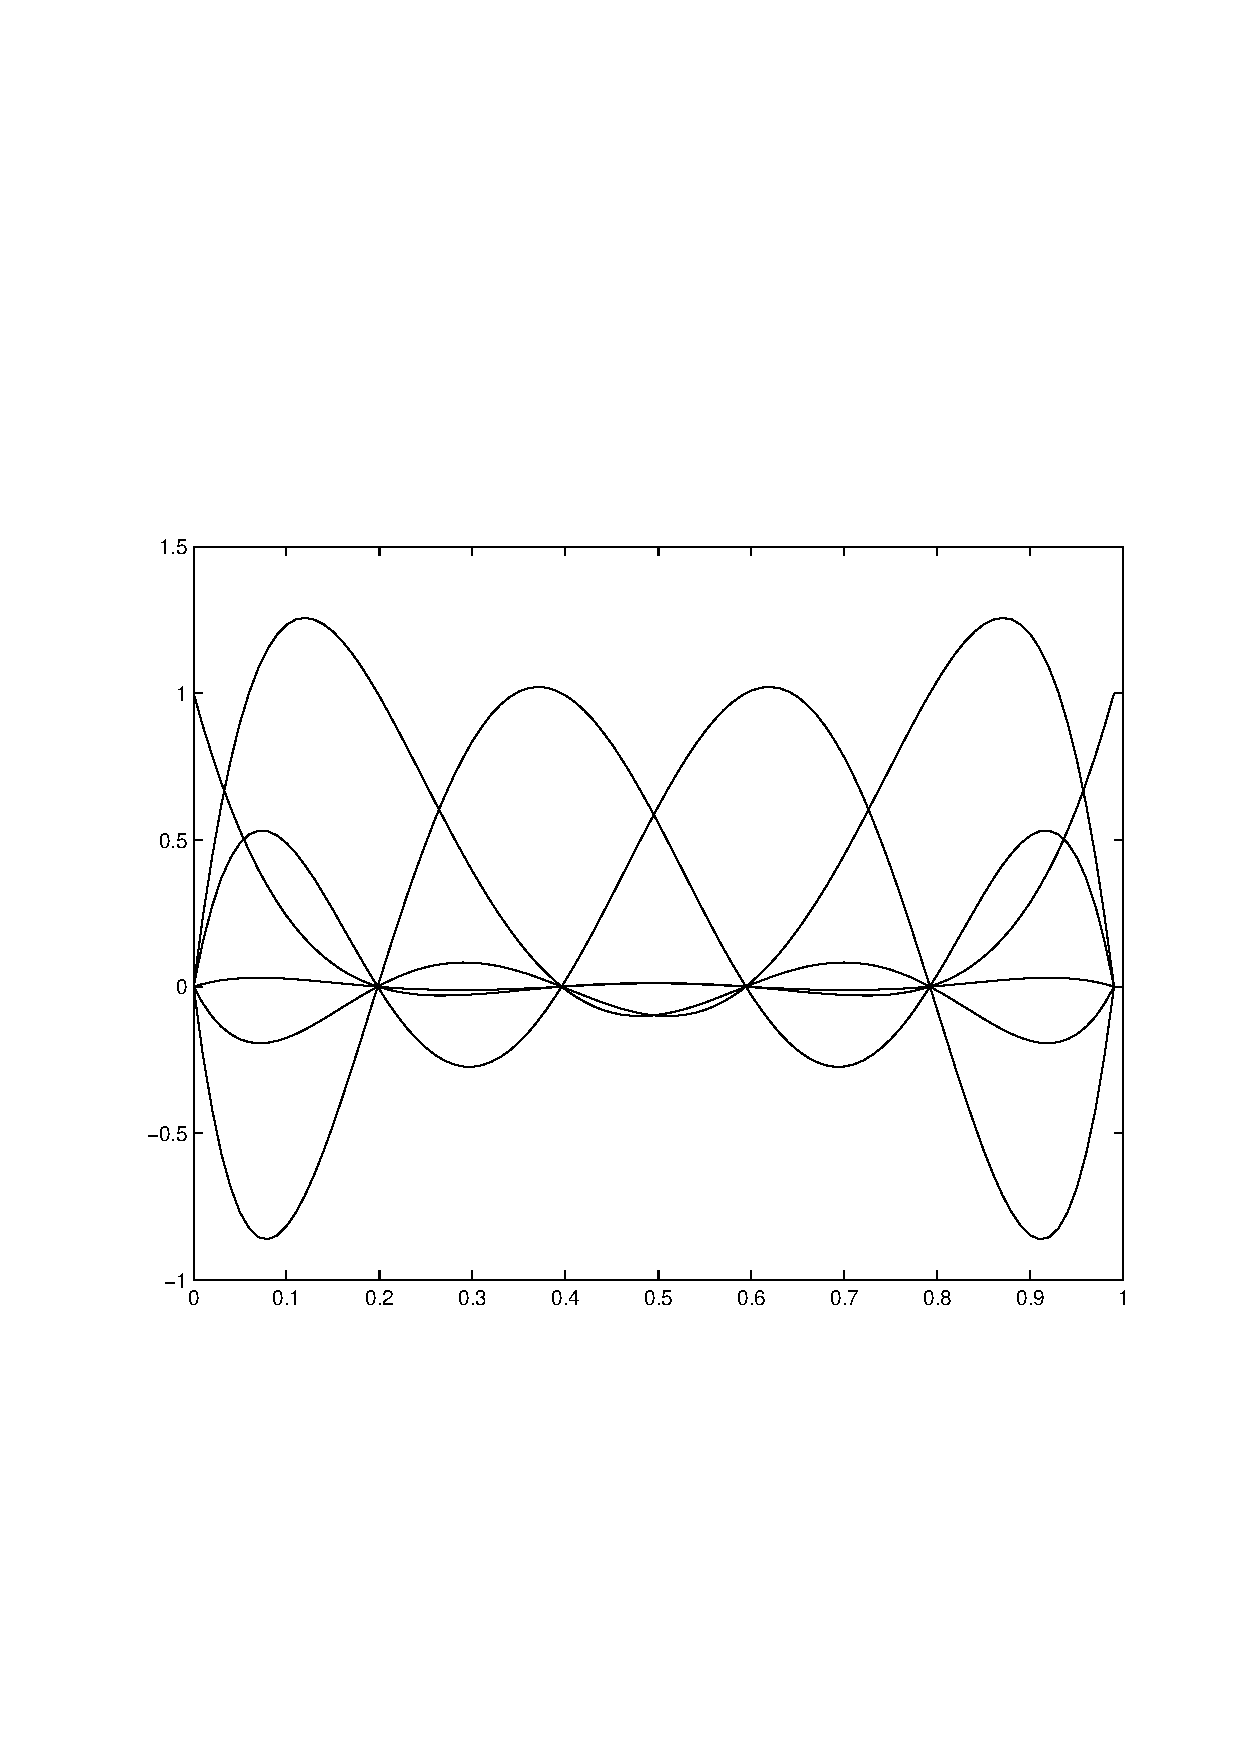
\includegraphics[width=4cm]{fempk51.pdf}}\htmlonly{\htmlimg{fempk51.png}{basis functions of the P5 fem}}

\par
Viewing the basis function of the Argyris FEM:
\begin{mcode}
f=gf_fem('FEM_ARGYRIS');
gf_fem_get(f, 'poly_str')
\end{mcode}
\end{cmdexamples}
\begin{gfseealso}
@@gf_fem@@
\end{gfseealso}
\newpage

%%%%%%%%%%%%%%%%%%%%%%% GF_INTEG
\subsection{gf\_integ}
\begin{purpose}
\hypertarget{gfinteg}
  General function for obtaining handles to various integrations
  methods on convexes (used when the elementary matrices are built)\index{integration method}.
\end{purpose}
\begin{synopsis}
@@\tinteg IM = gf\_integ(\tstr method)
@@\end{synopsis}
\begin{cmddescription}
  Here is a list of some integration methods defined in \gf (see the
   \WEB{http://www-gmm.insa-toulouse.fr/getfem/doc}{description of finite
    element and integration methods} for a complete reference):

  \begin{tabular}{|l|l|}
    \hline
    \kw{IM\_EXACT\_SIMPLEX(N)}       & exact integration on simplices.\\
    \kw{IM\_PRODUCT(a, b)}           & product of two integration methods\\
    \kw{IM\_EXACT\_PARALLELEPIPED(N)}& exact integration on parallelepipeds\\
    \kw{IM\_EXACT\_PRISM(n)}         & exact integration on prisms\\
    \kw{IM\_GAUSS1D(K)}              & Gauss method on the segment, order K\\
    \kw{IM\_NC(N,K)}                 & Newton-Cotes approximative integration on simplices, order K\\
    \kw{IM\_NC\_PARALLELEPIPED(N,K)} & product of Newton-Cotes integration on parallelepipeds\\
    \kw{IM\_NC\_PRISM(N,K)}          & product of Newton-Cotes integration on prisms\\
    \kw{IM\_GAUSS\_PARALLELEPIPED(N,K)}&  product of Gauss1D integration on parallelepipeds\\
    \kw{IM\_TRIANGLE(K)}             & Gauss methods on triangles $(K=1,3,5,6,7,8,9,10,13,17,19)$\\
    \kw{IM\_TETRAHEDRON(K)}          & Gauss methods on tetrahedrons (K=1, 2, 3, 5, 6 or 8)\\
    \hline
  \end{tabular}
   Note that 'exact integration'
      should be avoided in general, since they only apply to linear
      geometric transformations, are quite slow, and subject to
      numerical stability problems for high degree FEMs.
\end{cmddescription}
\begin{gfseealso}
  @@gf\_fem, gf\_mesh\_im, gfInteg@@.
\end{gfseealso}
\newpage

%%%%%%%%%%%%%%%%%%%%%%% GF_INTEG_GET
\subsection{gf\_integ_get}
\begin{purpose}
\hypertarget{gfintegget}
  Gives access to various internal informations of an Integration Method handle @@IM@@\index{integration method}.
\end{purpose}
\begin{synopsis}
@@\tint I = gf_integ_get(IM,'is_exact')
\tint I = gf_integ_get(IM,'dim')
\tint I = gf_integ_get(IM,'nbpts')
\tmat gf_integ_get(IM,'pts')
\tvec gf_integ_get(IM,'coeffs')
\tmat gf_integ_get(IM,'face_pts', \tint F)
\tvec gf_integ_get(IM,'face_coeffs',\tint F)
\tstr S=gf_integ_get(IM,'char')
@@\end{synopsis}
\begin{cmddescription}
  \sep{@@gf_integ_get(IM,'is_exact')@@} is non-null if the integration
  method is exact (i.e. integrates analytically polynomials). In that
  case there is not much information to obtain, except the dimension
  of the space on which it operates. For non-exact integration
  methods, \hil{@@gf_integ_get(IM,'pts')@@} and
  \hil{@@gf_integ_get(IM,'coeffs')@@} returns the points and
  coefficients of the quadrature formula for integrations over the
  whole convex, while \hil{@@gf_integ_get(IM,'face_pts', F)@@} and
  \hil{@@gf_integ_get(IM,'face_coeffs',F)@@} return the points and
  coefficients used for integrations over the face @@F@@ of the
  convex.
  
  \sep{@@gf_integ_get(IM,'char')@@} : return a string describing the integration
  method (similar to the one passed to @@gf_integ@@ for the creation of an
  integration method.
\end{cmddescription}
\begin{gfseealso}
@@gf_integ@@
\end{gfseealso}
\newpage

%%%%%%%%%%%%%%%%%%%%%%% GF_MESH_FEM
\subsection{gf\_mesh\_fem}
\begin{purpose}
\hypertarget{gfmeshfem}
General constructor for \tmf object. Returns a \gf handle 
 to the newly created \tmf object\index{mesh_fem}.
\end{purpose}
\begin{synopsis}
@@\tmf MF = gf\_mesh\_fem(\tmesh M [, \tint Qdim=1])
\tmf MF[,M] = gf\_mesh\_fem('load', \tstr filename[,\tmesh M])
\tmf MF[,M] = gf\_mesh\_fem('from string', \tstr S [,\tmesh M])
\tmf MF = gf\_mesh\_fem('clone', \tmf MF0)
@@\end{synopsis}
\begin{cmddescription}
  This function creates a \tmf object. These objects hold the finite
  element basis functions on a mesh : a finite element is assigned
  to each convex of the mesh, and the \tmf takes care of connecting
  them across the convexes and enumerating the degrees of freedom.


  \sep{@@gf\_mesh\_fem(M,Qdim)@@} creates a new \tmf object linked to the
  \tmesh @@M@@. \tmf objects can be used everywhere a \tcmesh object
  is required (its linked mesh is automatically used). The argument
  \kw{Qdim}\index{Qdim} specifies the dimension of the unknown on this
  mesh. If the unknown is a scalar field, then $\kw{Qdim}=1$, if it is
  a 2D vector field then $\kw{Qdim}=2$ etc\ldots: this is independent of
  the mesh dimension.
  
  The load command can restore a previously saved \tmf object. If you don't
  specify the \tmesh argument, it is assumed that the mesh was saved in the
  same file that the \tmf (with @@gf\_mesh\_fem\_get(mf, 'save with mesh')@@). The
  @@'from string'@@ command is very similar, but loads the object from a string
  instead of a file.

  And finally, it is possible to build a copy of a \tmf object with
  the \hil{@@gf\_mesh\_fem('clone', MF0)@@} command (see also the
  @@gf_mesh('clone')@@ command).
\end{cmddescription}
\begin{gfseealso}
  @@gf\_mesh\_fem\_get, gf\_mesh\_fem\_set, gfMeshFem@@
\end{gfseealso}
\newpage


%%%%%%%%%%%%%%%%%%%%%%% GF_MESH_FEM_GET
\subsection{gf\_mesh\_fem\_get}
\begin{purpose}
\hypertarget{gfmeshfemget}
  General inquiry function for \tmf objects\index{mesh_fem}.
\end{purpose}
\begin{synopsis}
@@\tint N = gf\_mesh\_fem\_get(MF, 'nbdof')
\tint N = gf\_mesh\_fem\_get(MF, 'nb basic dof')
\tivec DOF = gf\_mesh\_fem\_get(MF, 'basic dof from cv', \tivec CVLST)
\tivec [DOF,CV2DOF] = gf\_mesh\_fem\_get(MF, 'basic dof from cvid', [\tivec CVLST])
\tivec DOF = gf\_mesh\_fem\_get(MF, 'non conformal basic dof' [, \tivec CVLST])
\tfem FEMLST[, \tivec CV2F] = gf\_mesh\_fem\_get(MF, 'fem' [, \tivec CVLST])
\tivec CVLST = gf\_mesh\_fem\_get(MF, 'convex\_index')
\tint N = gf\_mesh\_fem\_get(MF, 'qdim')
\tivec I = gf\_mesh\_fem\_get(MF, \{'is\_lagrangian' | 'is\_equivalent' | 'is\_polynomial'\} 
        [, \tivec CVLST])
\tint N = gf\_mesh\_fem\_get(MF, 'is\_reduced')
\tspmat R = gf\_mesh\_fem\_get(MF, 'reduction\_matrix')
\tspmat R = gf\_mesh\_fem\_get(MF, 'extension\_matrix')
\tivec DOFLST = gf\_mesh\_fem\_get(MF, 'basic dof on region', \tivec rlist)
\tivec DOFLST = gf\_mesh\_fem\_get(MF, 'dof on region', \tivec rlist)
\tmat DOF\_XY = gf\_mesh\_fem\_get(MF, 'basic dof nodes'[, \tivec DOFLST])
\tivec DOFP = gf\_mesh\_fem\_get(MF, 'dof partition')
\tvec U = gf\_mesh\_fem\_get(MF, 'interpolate convex data', \tvec Ucv)
gf\_mesh\_fem\_get(MF, 'save', \tstr filename, ['with mesh'])
gf\_mesh\_fem\_get(MF,'export_to_vtk', filename, ... ['ascii'], U, 'name'...)
gf_mesh_fem_get(MF,'export_to_dx', filename, ... ['as', mesh_name][,'edges']['serie',serie_name][,'ascii'][,'append'], U, 'name'...)
\tstr S=gf_mesh_fem_get(M, 'char' [,'with mesh'])
\tmesh M=gf_mesh_fem_get(MF, 'linked mesh')
\tvec U=gf_mesh_fem_get(MF, 'eval', expr [,\tivec DOFLST])
M=gf_mesh_fem_get(MF, 'memsize')
@@\end{synopsis}
\begin{cmddescription}
  \sep{@@gf\_mesh\_fem\_get(MF, 'nbdof')@@} : return the number of degrees
  of freedom of the \tmf @@MF@@.

  \sep{@@gf\_mesh\_fem\_get(MF, 'nb basic dof')@@} : return the number of
  basic degrees of freedom of the \tmf @@MF@@.

  \sep{@@gf\_mesh\_fem\_get(MF, 'basic dof from cv', CVLST)@@} :
  \index{dof}\index{degrees of freedom} return the basic dof IDs attached to
  the convexes listed in @@CVLST@@. WARNING: the Degrees of Freedom
  might be returned in ANY order, do not use this function in your
  assembly routines. Use @@'basic dof from cvid'@@ instead.

  \sep{@@gf\_mesh\_fem\_get(MF, 'dof from cv', rlist)@@} : Deprecated
  function. Use @@gf\_mesh\_fem\_get(MF, 'basic dof from cv', rlist)@@ instead.
  
  \sep{@@gf\_mesh\_fem\_get(MF, 'basic dof from cvid' [, CVLST])}@@ : return
  the degrees of freedom attached to each convex of the mesh, allowing
  to map a convex number to the list of its associated degrees of
  freedom. It is similar to @@gf\mesh\_get(M, 'pid from cvid')@@.

  \sep{@@gf\_mesh\_fem\_get(MF, 'dof from cvid', rlist)@@} : Deprecated
  function. Use @@gf\_mesh\_fem\_get(MF, 'basic dof from cvid', rlist)@@ instead.

  \sep{@@gf\_mesh\_fem\_get(MF, 'non conformal basic dof' [, CVLST])@@} :
  return the list of basic DoF which are located on the border of a convex
  and which belong to only one convex, except those who lie on the
  border of the mesh. For example, if the convex $a$ and $b$ share a
  common face, $a$ has a P1 FEM, and $b$ has a P2 FEM, then the basic dof on
  the middle of the common face will be returned by this function
  (this can be useful when searching the interfaces between classical
  fems and hierarchical fem).

  \sep{@@gf\_mesh\_fem\_get(MF, 'non conformal dof', rlist)@@} : Deprecated
  function. Use @@gf\_mesh\_fem\_get(MF, 'non conformal basic dof', rlist)@@ instead.

  \sep{@@gf\_mesh\_fem\_get(MF, \str{Qdim})@@}\index{Qdim} : return the
  dimension @@Q@@ of the fields interpolated by the \tmf (1 for scalar
  fields, 2 for 2D vector fields etc..)..
  
  \sep{@@FEMLST[, CV2F] = gf\_mesh\_fem\_get(MF, 'fem' [, \tivec
    CVLST])@@} : \index{FEM} return a list of \tfem objects:
  @@FEMLST@@ is an array of all \tfem objects found in the convexes
  given in @@CVLST@@. If @@CV2F@@ was supplied as an output argument,
  it contains, for each convex listed in @@CVLST@@, the index of its
  corresponding \tfem in @@FEMLST@@.

  Convexes which are not part of the mesh, or convexes which do not
  have any FEM have their correspounding entry in CV2F set to -1.

  \sep{@@gf\_mesh\_fem\_get(MF, 'convex\_index')@@} : 
  return the list of convexes who have a FEM.

  \sep{@@gf\_mesh\_fem\_get(MF, \{'is\_lagrangian' | 'is\_equivalent' |
    'is\_polynomial'\},[, CVLST])@@} :
  \index{Lagrangian}\index{equivalent FEM}\index{polynomial FEM} test
  the properties of the FEM of the convexes listed in @@CVLST@@.  If
  @@CVLST@@ is omitted, it returns 1 if all convexes in the mesh which
  are lagrangian (resp.  equivalents, resp. polynomials), or 0.  If
  @@CVLST@@ is present, returns the convex numbers (with respect to
  @@CVLST@@) which are lagrangian (resp. etc..)

  \sep{@@gf\_mesh\_fem\_get(MF, 'is\_reduced')@@} : 
  return 1 if the optional reduction matrix is applied to the dofs

  \sep{@@gf\_mesh\_fem\_get(MF, 'reduction\_matrix')@@} : 
  return the optional reduction matrix.

  \sep{@@gf\_mesh\_fem\_get(MF, 'extension\_matrix')@@} : 
  return the optional extension matrix.

  \sep{@@gf\_mesh\_fem\_get(MF, 'basic dof on region', rlist)@@} : return the
  list of basic dof (i.e. before optional reduction) whose support is
  non-null on one of the regions whose
  ids are listed in @@rlist@@ (note that for boundary regions, some
  basic dof nodes may not lie exactly on the boundary, for example the dof
  of @@FEM_PK(n,0)@@ lies on the center of the convex, but the base
  function in not null on the convex border).

  \sep{@@gf\_mesh\_fem\_get(MF, 'dof on region', rlist)@@} : return the
  list of dof (i.e. after optional reduction) whose support is
  non-null on one of the regions whose
  ids are listed in @@rlist@@ (note that for boundary regions, some
  basic dof nodes may not lie exactly on the boundary, for example the dof
  of @@FEM_PK(n,0)@@ lies on the center of the convex, but the base
  function in not null on the convex border).
  
  For a reduced mesh\_fem
  a dof is lying on a region if its potential corresponding shape
  function is nonzero on this region. The extension matrix is used
  to make the correspondance between basic and reduced dofs

  \sep{@@gf\_mesh\_fem\_get(MF, 'dof on region', rlist)@@} : Deprecated
  function. Use @@gf\_mesh\_fem\_get(MF, 'basic dof on region', rlist)@@ instead.

  \sep{@@gf\_mesh\_fem\_get(MF, 'basic dof nodes'[, DOFLST])@@} : return the
  list of interpolation points for the specified basic dof IDs in @@DOFLST@@
  (if @@DOFLST@@ is omitted, all basic dof are considered).

  \sep{@@gf\_mesh\_fem\_get(MF, 'dof nodes', rlist)@@} : Deprecated
  function. Use @@gf\_mesh\_fem\_get(MF, 'basic dof nodes', rlist)@@ instead.

  \sep{@@gf\_mesh\_fem\_get(MF, 'dof partition')@@} : return the array
  which associates an integer (the partition number) to each convex of
  the \tmf. By default, it is an all-zero array.  The degrees of
  freedom of each convex are connected only to the dof of neighbouring
  convexes which have the same partition number, hence it is possible
  to create partially discontinuous mesh_fem very easily.


  \sep{@@gf\_mesh\_fem\_get(MF, 'interpolate convex data', Ucv)@@} is a
  convenient function to interpolate quickly some data that is given
  on the mesh convexes (for example the output of @@gf\_mesh\_get(m,
  'quality')@@) on @@MF@@ (a similar function also exists for slices).
  Note that it works better if @@MF@@ is a discontinuous \tmf (for
  example @@'FEM_PK(N,0)'@@), or the result will be ``smoothed''.

  
  \sep{@@gf\_mesh\_fem\_get(MF, 'save', filename [,'with mesh'])@@} : save the \tmf\ in a
  text file (which can be loaded later with @@gf\_mesh\_fem(m, 'load',
  filename)@@. Please note that the associated mesh is not saved, except if you
  use the @@'with mesh'@@ option! @@gf_mesh_fem_get(M, 'char' [,'with mesh'])@@
  is similar, but saves the content of the \tmf in a string.

  \sep{@@gf_mesh_fem_get(MF, 'char')@@} : get a string description of the \tmf.

  \sep{@@gf\_mesh\_fem\_get(MF,'export_to_vtk', filename, ... ['ascii'], U, 'name'...)@@} : 
  export a \tmf and some fields to a \VTK file.  The FEM and geometric
    transformations will be mapped to order 1 or 2 isoparametric PK (or QK) FEMs
    (as \VTK does not handle higher order elements). If you need to represent high-
    order FEMs or high-order geometric transformations, you should consider
    @@gf_slice_get(sl,'export_to_vtk')@@.

    \sep{@@gf_mesh_fem_get(MF,'export_to_dx', filename, ... ['as', mesh_name][,'edges']['serie',serie_name][,'ascii'][,'append'], U, 'name'...)@@} :
    export a mesh_fem and some fields to an \OpenDX file.  This function will fail
    if the \tmf mixes different convex types (i.e. quads and triangles), or
    if \OpenDX does not handle a specific element type (i.e. prism connections are
    not known by \OpenDX).  The FEM will be mapped to order 1 PK (or QK) FEMs. If
    you need to represent high-order FEMs or high-order geometric transformations,
    you should consider @@gf_slice_get(sl,'export_to_dx')@@.


    \sep{@@gf_mesh_fem_get(MF, 'linked mesh')@@} return an handle to the mesh object
  linked to @@MF@@.

  \sep{@@gf_mesh_fem_get(MF, 'eval', expr [,DOFLST])@@} : call @@gf_mesh_fem_get_eval@@. This function interpolates an expression on a lagrangian \tmf (for all dof except if @@DOFLST@@ is specified). The expression can be a numeric constant, or a cell array containing numeric constants, string expressions or function handles. For example:
  \begin{mcode}
U1=gf_mesh_fem_get(mf,'eval',1)
U2=gf_mesh_fem_get(mf,'eval',[1;0]) % output has two rows
U3=gf_mesh_fem_get(mf,'eval',[1 0]) % output has one row, only valid if qdim(mf)==2
U4=gf_mesh_fem_get(mf,'eval',\{'x';'y.*z';4;@myfunctionofxyz\})
  \end{mcode}

  \sep{@@gf_mesh_fem_get(M, 'memsize')@@} : return the amount of
  memory (in bytes) used by the \tmf object (the linked mesh is not
  counted).
\end{cmddescription}
\begin{gfseealso}
  \kwl{gfmeshget}{gf\_mesh\_get}, \kwl{gfmeshset}{gf\_mesh\_set}
\end{gfseealso}
\newpage


%%%%%%%%%%%%%%%%%%%%%%% GF_MESH_FEM_SET
\subsection{gf\_mesh\_fem\_set}
\begin{purpose}
\hypertarget{gfmeshfemset}
  General function for editing \tmf\ objects\index{mesh_fem}.
\end{purpose}
\begin{synopsis}
@@gf\_mesh\_fem\_set(MF, 'fem', \tfem fem [, \tivec CVIDX])
gf\_mesh\_fem\_set(MF, 'classical fem', \tfem fem, \tint K [, \tivec CVIDX])
gf\_mesh\_fem\_set(MF, 'classical discontinuous fem', \tfem fem, \tint K [, \tivec CVIDX])
gf\_mesh\_fem\_set(MF, 'qdim', \tint Qdim)
gf\_mesh\_fem\_set(MF, 'reduction', \tint s)
gf\_mesh\_fem\_set(MF, 'reduction matrices', \tspmat R, \tspmat E)
gf\_mesh\_fem\_set(MF, 'dof partition', \tivec DOFP)
@@\end{synopsis}
\begin{cmddescription}
  \sep{@@gf\_mesh\_fem\_set(MF, 'fem', fem [, CVIDX])@@} \index{FEM}
  set the finite element method to @@fem@@ for all
  the convexes listed in @@CVIDX@@ in the mesh linked to @@MF@@. If @@CVIDX@@ is not used,
  the @@fem@@ is assigned to all convexes. 
  
  \sep{@@gf\_mesh\_fem\_set(MF, 'classical fem', fem, K , [, CVIDX])@@} :
  set the classical fem (polynomial and Lagrange) of order @@K@@ on the
  listed convexes ($P_K$ for simplexes, $Q_K$ for parallelepipeds,
  etc..). 

  \sep{@@gf\_mesh\_fem\_set(MF, 'classical discontinuous fem', K [, CVIDX])@@} is
  similar to the previous one, but for discontinuous (i.e.
  @@'FEM_PK_DISCONTINUOUS'@@ etc) FEMs. This can be useful to
  interpolate the gradient of a continuous \tmf (which will be
  discontinuous across elements, except if you are using a C1 element
  such as Argyris or HCT).
  
  \sep{@@gf\_mesh\_fem\_set(MF, 'qdim', Qdim)@@} : \index{Qdim}
  change the @@Q@@ dimension of the field that is interpolated by the \tmf.
  @@Q=1@@ means that the \tmf describes a scalar field, @@Q=N@@ means
  that the \tmf describes a vector field of dimension @@N@@ (see @@gf_mesh_fem_set('Qdim')@@).

  \sep{@@gf\_mesh\_fem\_set(MF, 'reduction', s)@@} :
  Set or unset the use of reduction/extension matrices.

  \sep{@@gf\_mesh\_fem\_set(MF, 'reduction matrices', R, E)@@} :
  Set the reduction and extension matrices and valid their use.

  \sep{@@gf\_mesh\_fem\_set(MF, 'dof partition', \tivec DOFP)@@} : 
  change the array which associates an integer (the partition number) to each convex of
  the \tmf (see @@gf\_mesh\_fem\_get(MF, 'dof partition')@@).
\end{cmddescription}
\begin{cmdexamples}
  Building a discontinuous \tmf @@mfdu@@ to compute the gradient @@DU@@ of a field @@U@@ defined on a \tmf @@mf@@:
\begin{mcode}
mfdu=gfMeshFem(m);
% use polynomials of degree 2, and no integration method
gf_mesh_fem_set(mfdu,'classical discontinuous fem',2); 
DU=gf_compute(mf,U,'gradient',mfdu);
\end{mcode}
\end{cmdexamples}
\begin{gfseealso}
  @@gf\_mesh\_fem, gf_mesh_fem_set, gf_fem, gf_integ@@.
\end{gfseealso}
\newpage



%%%%%%%%%%%%%%%%%%%%%%% GF_MESH_IM
\subsection{gf\_mesh\_im}
\begin{purpose}
\hypertarget{gfmeshim}
General constructor for \tmim object. Return a \gf handle 
 to the newly created \tmim object\index{mesh_im}.
\end{purpose}
\begin{synopsis}
@@\tmim MIM = gf\_mesh\_im(\tmesh M [, \{ \tinteg | \tint \}])
\tmim MIM[,M] = gf\_mesh\_im('load', \tstr filename[,\tmesh M])
\tmim MIM[,M] = gf\_mesh\_im('from string', \tstr S [,\tmesh M])
\tmim MIM = gf\_mesh\_im('clone', \tmim MIM0)
@@\end{synopsis}
\begin{cmddescription}
  This function creates a \tmim object. These objects hold integration
  methods defined over a mesh: an \tmim object is required for each
  operation with needs integration of something over the mesh
  (assembly functions, etc.).

  \sep{@@gf\_mesh\_im(M [, { \tinteg IM | \tint IM_DEGREE}])@@} creates a new \tmim object linked to the \tmesh @@M@@. \tmim objects can be used everywhere a \tcmesh object is
  required (its linked mesh is automatically used). 

  As a convenience, an integration method can be applied immediately
  to all convexes of the mesh if the optional argument @@IM@@ or
  @@IM_DEGREE@@ is used (@@IM_DEGREE@@ let getfem choose a suitable
  integration method that is able to exactly integrate polynomials of
  degree less or equal to @@IM_DEGREE@@.
  
  The load command can restore a previously saved \tmim object. If you
  don't specify the \tmesh argument, it is assumed that the mesh was
  saved in the same file that the \tmim (with @@gf\_mesh\_im\_get(mf,
  'save with mesh')@@). The @@'from string'@@ command is very similar,
  but loads the object from a string instead of a file.

  @@gf\_mesh\_im('clone', MIM0)@@ return a copy of @@MIM0@@.
\end{cmddescription}
\begin{gfseealso}
  @@gf\_mesh\_im\_get, gf\_mesh\_im\_set, gfMeshIm@@
\end{gfseealso}
\newpage


%%%%%%%%%%%%%%%%%%%%%%% GF_MESH_IM_GET
\subsection{gf\_mesh\_im\_get}
\begin{purpose}
\hypertarget{gfmeshimget}
  General inquiry function for \tmim objects\index{mesh_im}.
\end{purpose}
\begin{synopsis}
@@\tstr IMLST[, \tivec CV2IM] = gf\_mesh\_im\_get(MIM, 'integ' [, \tivec CVLST])
\tivec CVLST = gf\_mesh\_im\_get(MIM, 'convex\_index')
\tmat M = gf\_mesh\_fem\_get(MIM, 'eltm', \teltm MET, \tint CV [, \tint FACE])
gf\_mesh\_im\_get(MIM, 'save', \tstr filename, ['with mesh'])
\tstr S=gf_mesh_im_get(M, 'char' [,'with mesh'])
\tmesh M=gf_mesh_im_get(MIM, 'linked mesh')
M=gf_mesh_im_get(MIM, 'memsize')
@@\end{synopsis}
\begin{cmddescription}
  \sep{@@IMLST[,CV2IM]=gf\_mesh\_im\_get(MIM, 'integ' [, \tivec
    CVLST])@@} : \index{integration method} return a list of \tinteg
  objects: @@IMLST@@ is an array of all \tinteg objects found in the
  convexes given in @@CVLST@@. If @@CV2IM@@ was supplied as an output
  argument, it contains, for each convex listed in @@CVLST@@, the
  index of its corresponding \tinteg in @@IMLST@@.

  Convexes which are not part of the mesh, or convexes which do
  not have any integration method have their correspounding entry
  in CV2I set to -1.

  \sep{@@gf\_mesh\_im\_get(MIM, 'convex\_index')@@} :
  return the list of convexes who have a integration method. Convexes
  who have the dummy @@IM_NONE@@ method are not listed.

  \sep{@@gf\_mesh\_im\_get(MIM, 'eltm', MET, CV [,F])@@} :
  \index{elementary matrix} return the elementary matrix (or tensor)
  integrated on the convex @@CV@@ for the elementary matrix type
  @@MET@@ (created with @@gf_eltm@@).  If @@F@@ is given, the
  elementary matrix is integrated on the face @@F@@ of convex @@CV@@.

  \sep{@@gf\_mesh\_im\_get(MIM, 'save', filename [,'with mesh'])@@} : save the \tmim\ in a
  text file (which can be loaded later with @@gf\_mesh\_im(m, 'load',
  filename)@@. Please note that the associated mesh is not saved, except if you
  use the @@'with mesh'@@ option! @@gf_mesh_im_get(M, 'char' [,'with mesh'])@@
  is similar, but saves the content of the \tmim in a string.
  
  \sep{@@gf_mesh_im_get(MIM, 'linked mesh')@@} : return an handle to the mesh object
  linked to @@MIM@@.

  \sep{@@gf_mesh_im_get(MIM, 'memsize')@@} : return the amount of memory (in bytes)
  used by the \tmim object (the linked mesh is not counted).
\end{cmddescription}
\newpage


%%%%%%%%%%%%%%%%%%%%%%% GF_MESH_IM_SET
\subsection{gf\_mesh\_im\_set}
\begin{purpose}
\hypertarget{gfmeshimset}
  General function for editing \tmim\ objects\index{mesh_im}.
\end{purpose}
\begin{synopsis}
@@gf\_mesh\_im\_set(MIM, 'integ', \{ \tinteg im | \tint IMDEGREE \}, [, \tivec CVIDX])@@\end{synopsis}
\begin{cmddescription}
  \sep{@@gf\_mesh\_im\_set(MIM, 'integ', im [, CVIDX])@@} : \index{IM}
  set @@im@@ as the integration method for all
  the convexes listed in @@CVIDX@@ in the mesh linked to @@MF@@. If @@CVIDX@@ is not used,
  the @@im@@ is assigned to all convexes. 
  
  \sep{@@gf\_mesh\_im\_set(MIM, 'integ', IM\_DEGREE [, CVIDX])@@} :
  assign a classical approximate integration method of order at least @@IM_DEGREE@@ on the
  listed convexes. If @@IM_DEGREE@@=-1, then the dummy integration method
  @@'IM_NONE'@@ is used.
\end{cmddescription}
\begin{cmdexamples}
\begin{mcode}
mim=gfMeshIm(m);
% set an integration method of order 5 on all convexes
gf_mesh_im_set(mim,'integ',5); 
% change the integration for convexes 5 6 9
gf_mesh_im_set(mim,'integ',gf_integ('IM_TRIANGLE(13)'),[6 5 9]);
\end{mcode}
\end{cmdexamples}
\newpage


%%%%%%%%%%%%%%%%%%%%%%% GF_MDBRICK
\subsection{gf\_mdbrick}
\begin{purpose}
\hypertarget{gfmdbrick}
General constructor for \tmdbrick objects. Return a \gf handle 
 to the newly created \tmdbrick object\index{mdbrick}.
\end{purpose}
\begin{synopsis}
@@gf_mdbrick('constraint', \tmdbrick parent, \tstr CTYPE [, \tint numfem])
gf_mdbrick('dirichlet', \tmdbrick parent, \tint BNUM, \tmf MFMULT, \tstr CTYPE
          [, \tint numfem])
gf_mdbrick('dirichlet on normal component', \tmdbrick parent, \tint BNUM, \tmf MFMULT,
          \tstr CTYPE [, \tint numfem])
gf_mdbrick('dirichlet on normal derivative', \tmdbrick parent, \tint BNUM, \tmf MFMULT, 
          \tstr CTYPE [, \tint numfem])
gf_mdbrick('generalized dirichlet', \tmdbrick parent, \tint BNUM [, \tint numfem])
gf_mdbrick('source term', \tmdbrick parent, [, \tint BNUM=-1[, \tint numfem]])
gf_mdbrick('normal source term', \tmdbrick parent, \tint BNUM [, \tint numfem])
gf_mdbrick('normal derivative source term', \tmdbrick parent, \tint BNUM [, \tint numfem])
gf_mdbrick('neumann KirchhoffLove source term', \tmdbrick parent, \tint BNUM [, \tint numfem])
gf_mdbrick('qu term', \tmdbrick parent, [, \tint BNUM [, \tint numfem]])
gf_mdbrick('mass matrix', \tmim mim, \tmf mf_u [,'real'|'complex'])
gf_mdbrick('generic elliptic', \tmim MIM, \tmf mfu 
          [,'scalar'|'matrix'|'tensor'][,'real'|'complex'])
gf_mdbrick('helmholtz', \tmim MIM, \tmf mfu [,'real'|'complex'])
gf_mdbrick('isotropic linearized elasticity', \tmim MIM, \tmf mfu)
gf_mdbrick('linear incompressibility term', \tmdbrick parent, \tmf mf_p [, \tint numfem])
gf_mdbrick('nonlinear elasticity', \tmim MIM, \tmf mfu, \tstr lawname)
gf_mdbrick('nonlinear elasticity incompressibility term', \tmdbrick parent, 
          \tmf mf_p [, \tint numfem])
gf_mdbrick('small deformations plasticity', \tmim MIM, \tmf mfu, \tscal THRESHOLD)
gf_mdbrick('bilaplacian', \tmim MIM, \tmf mfu, ['Kirchhoff-Love'])

gf_mdbrick('isotropic_linearized_plate', \tmim MIM, \tmim MIMSUB, \tmf MF_UT, \tmf MF_U3, \tmf MF_THETA, \tscal EPSILON)
gf_mdbrick('mixed_isotropic_linearized_plate', \tmim MIM, \tmf MF_UT, \tmf MF_U3, \tmf MF_THETA, \tscal EPSILON)
gf_mdbrick('plate_source_term', \tmdbrick parent, [, \tint BNUM=-1[, int numfem]])
gf_mdbrick('plate_simple_support', \tmdbrick parent, \tint BNUM, \tstr CTYPE [, \tint numfem])
gf_mdbrick('plate_clamped_support', \tmdbrick parent, \tint BNUM, \tstr CTYPE[, \tint numfem])
gf_mdbrick('plate_closing', \tmdbrick parent [, \tint numfem])

@@\end{synopsis}
\begin{cmddescription}
  Many of the bricks take a @@numfem@@ optional parameter, which
  is the \mf number in the stack of parent bricks (by default
  @@numfem=0@@, i.e. it refers to the first meshfem in the stack of
  bricks).

\sep{@@gf_mdbrick('constraint', parent, CTYPE [, numfem])@@}
 : build a generic constraint brick. 

It may be useful in some situations, such as the Stokes problem
where the pressure in defined modulo a constant. In such a
situation, this brick can be used to add an additional
constraint on the pressure value.      
@@CTYPE@@ has to be chosen among @@'augmented'@@, @@'penalized'@@, and
@@'eliminated'@@.  The constraint can be specified with
@@gf_mdbrick_set('constraints')@@. Note that Dirichlet bricks (except the
'generalized Dirichlet' one) are also specializations of the
'constraint' brick.

\sep{@@gf_mdbrick('dirichlet', \tmdbrick parent, \tint BNUM, \tmf MFMULT, \tstr CTYPE [, \tint numfem])@@}
: build a Dirichlet condition brick which impose the value of a field along a mesh boundary.
      
The @@BNUM@@ parameter selects on which mesh region the Dirichlet
condition is imposed. @@CTYPE@@ has to be chosen among @@'augmented'@@, @@'penalized'@@, and @@'eliminated'@@. The @@MFMULT@@ may generally be taken
as the \mf of the unknown, but for 'augmented' Dirichlet
conditions, you may have to respect the Inf-Sup condition and
choose an adequate \mf.

\sep{@@gf_mdbrick('dirichlet on normal component', parent, BNUM, MFMULT, CTYPE [, numfem])@@}
 : build a Dirichlet condition brick which imposes the value of the normal component of a vector field.

\sep{@@gf_mdbrick('dirichlet on normal derivative', parent, BNUM, MFMULT, CTYPE [, numfem])@@}
 : build a Dirichlet condition brick which imposes the value of the normal derivative of the unknown.

\sep{@@gf_mdbrick('generalized dirichlet', parent, BNUM [, numfem])@@} : this is the "old" Dirichlet brick of getfem. 
      
This brick can be used to impose general Dirichlet conditions
$h(x)u(x) = r(x)$ , however it may have some issues with elaborated FEM (such as Argyris, etc). It should be avoided when possible.


\sep{@@gf_mdbrick('source term', parent, [, BNUM=-1[, numfem]])@@}
 : add a boundary or volumic source term ( $\int B.v$ ).

If @@BNUM@@ is omitted (or set to -1) , the brick adds a volumic
source term on the whole mesh. For @@BNUM >= 0@@, the source term is
imposed on the mesh region @@BNUM@@. Use @@gf_mdbrick_set('param','source
term',mf,B)@@ to set the source term field. The source term is
expected as a vector field of size Q (with Q = qdim).

\sep{@@gf_mdbrick('normal source term', parent, BNUM [, numfem])@@}
 : add a boundary source term ( $\int (Bn).v$ ).

The source term is imposed on the mesh region @@BNUM@@ (which of
course is not allowed to be a volumic region, only boundary
regions are allowed). Use @@gf_mdbrick_set('param','source term',mf,B)@@
to set the source term field. The source term @@B@@ is expected as
tensor field of size $QxN$ (with $Q$ = qdim, $N$ = mesh dim). For
example, if you consider an elasticity problem, this brick may
be used to impose a force on the boundary with @@B@@ as the stress
tensor.

\sep{@@gf_mdbrick('normal derivative source term', parent, BNUM [, numfem])@@}
 : add a boundary source term ( $\int (\partial_n B).v$ ).

The source term is imposed on the mesh region @@BNUM@@.  Use
@@gf_mdbrick_set('param','source term',mf,B)@@ to set the source term
field, which is expected as a vector field of size $Q$ (with $Q$ =
qdim).

\sep{@@gf_mdbrick('neumann KirchhoffLove source term', parent, BNUM [, numfem])@@} : add a boundary source term for neumann Kirchhoff-Love
plate problems (should be used with the Kirchhoff-Love flavour of the
bilaplacian brick).

\sep{@@gf_mdbrick('qu term', parent, [, BNUM [, numfem]])@@}
 : update the tangent matrix with a $\int (Qu).v$ term.

The $Q(x)$ parameter is a matrix field of size @@qdim x qdim@@. An
example of use is for the "iku" part of Robin boundary conditions
$\partial_n u + iku = ...$

\sep{@@gf_mdbrick('mass matrix', mim, mf_u [,'real'|'complex'])@@}
 : build a mass-matrix brick.

\sep{@@gf_mdbrick('generic elliptic', MIM, mfu [,'scalar'|'matrix'|'tensor'][,'real'|'complex'])@@}
 : setup a generic elliptic problem ( $\int (A(x)\nabla u).\nabla v$ )

The brick parameter @@'A'@@ may be a scalar field, a matrix field, or a tensor field (default is scalar, and $A=1$).

\sep{@@gf_mdbrick('helmholtz', MIM, mfu [,'real'|'complex'])@@}
 : setup a Helmholtz problem. The brick has one parameter, @@'wave_number'@@.

\sep{@@gf_mdbrick('isotropic linearized elasticity', MIM, mfu)@@}
 : setup a linear elasticity problem.
      The brick has two scalar parameter, @@'lambda'@@ and @@'mu'@@ (the Lam\'e coefficients).

\sep{@@gf_mdbrick('linear incompressibility term', parent, mf_p [, numfem])@@} :
add an incompressibily constraint ($\nabla.u = 0$).

\sep{@@gf_mdbrick('nonlinear elasticity', MIM, mfu, lawname)@@} : 
setup a nonlinear elasticity (large deformations) problem.

The material law can be chosen among
\begin{itemize}
  \item @@'SaintVenant Kirchhoff'@@ (linearized material law)
  \item @@'Mooney Rivlin'@@ (to be used with the nonlinear incompressibily term)
  \item @@'Ciarlet Geymonat'@@
\end{itemize}


\sep{@@gf_mdbrick('nonlinear elasticity incompressibility term', parent, mf_p [, numfem])@@} :
add an incompressibily constraint to a large strain elasticity problem.

\sep{@@gf_mdbrick('small deformations plasticity', MIM, mfu, @scalar THRESHOLD)@@} : 
setup a plasticity problem (with small deformations).

The @@THRESHOLD@@ parameter is the maximum value of the Von Mises
stress before ``plastification'' of the material.

\sep{@@gf_mdbrick('bilaplacian', MIM, mfu, ['Kirchhoff-Love'])@@}
 : setup a bilaplacian problem.

If the Kirchhoff-Love option is specified, the Kirchhoff-Love
plate model is used.

@@gf_mdbrick('isotropic_linearized_plate', MIM, MIMSUB, MF_UT, MF_U3, MF_THETA, EPSILON)@@

setup a linear plate model brick (for moderately thick plates, using
the Reissner-Mindlin model). @@EPSILON@@ is the plate thinkness, the \mf
@@MF_UT@@ and @@MF_U3@@ are used respectively for the membrane displacement
and the transverse displacement of the plate. The \mf @@MF_THETA@@ is the
rotation of the normal ("section rotations").  The second integration
method @@MIMSUB@@ can be chosen equal to @@MIM@@, or different if you want to
perform sub-integration on the transverse shear term (mitc4
projection).  This brick has two parameters "lambda" and "mu" (the Lam\'e
coefficients)

@@gf_mdbrick('mixed_isotropic_linearized_plate', MIM, MF_UT, MF_U3, MF_THETA, EPSILON)@@

setup a mixed linear plate model brick (for thin plates, using
Kirchhoff-Love model).  For a non-mixed version, use the bilaplacian
brick.

@@gf_mdbrick('plate_source_term', parent, [, BNUM=-1[, numfem]])@@

add a boundary or a volumic source term to a plate problem. This brick
has two parameters: "B" is the displacement (ut and u3) source term,
"M" is the moment source term (i.e. the source term on the rotation of
the normal).

@@gf_mdbrick('plate_simple_support', parent, BNUM, CTYPE [, numfem])@@

add a "simple support" boundary condition to a plate problem (homogeneous
Dirichlet condition on the displacement, free rotation). @@CTYPE@@ specifies how
the constraint is enforced ('penalized', 'augmented' or 'eliminated').


@@gf_mdbrick('plate_clamped_support', parent, BNUM, CTYPE[, numfem])@@

add a "clamped support" boundary condition to a plate problem
(homogeneous Dirichlet condition on the displacement and on the
rotation).

@@gf_mdbrick('plate_closing', parent [, numfem])@@
add a free edges condition for the mixed plate model brick.  This brick is
required when the mixed linearized plate brick is used. It must be inserted
after all other boundary conditions (the reason is that the brick has to
inspect all other boundary conditions to determine the number of disconnected
boundary parts which are free edges).

\end{cmddescription}
\newpage

%%%%%%%%%%%%%%%%%%%%%%% GF_MDBRICK_GET
\subsection{gf\_mdbrick_get}
\begin{purpose}
\hypertarget{gfmdbrickget}
Query information on a \tmdbrick \index{mdbrick} object @@b@@.
\end{purpose}
\begin{synopsis}
@@\tint n = gf_mdbrick_get(b,'nbdof')
\tint n = gf_mdbrick_get(b, 'dim')
\tint gf_mdbrick_get(b, 'is_linear')
\tint gf_mdbrick_get(b, 'is_symmetric')
\tint gf_mdbrick_get(b, 'is_coercive')
\tint gf_mdbrick_get(b, 'is_complex')
\tivec I=gf_mdbrick_get(b, 'mixed_variables')
\tstr gf_mdbrick_get(b, 'subclass')
LST=gf_mdbrick_get(b, 'param_list')
\tvec gf_mdbrick_get(b,'param', \tstr parameter_name)
gf_mdbrick_get(b,'solve', \tmdstate mds [,...])
\tvec VM=gf_mdbrick_get(b, 'von_mises', \tmdstate mds, \tmf MFVM)
\tvec VM=gf_mdbrick_get(b, 'tresca', \tmdstate mds, \tmf MFVM)@@
\end{synopsis}
\begin{cmddescription}    
  \sep{@@gf_mdbrick_get(b,'nbdof')@@} : et the total number of dof of
  the current problem.  This is the sum of the brick specific dof plus
  the dof of the parent bricks.

  \sep{@@gf_mdbrick_get(b,'dim')@@} : get the dimension of the main
  mesh (2 for a 2D mesh, etc).

  \sep{@@gf_mdbrick_get(b,'is_linear')@@} : return true if the problem (this brick plus its parent bricks) is linear.
  
  \sep{@@gf_mdbrick_get(b,'is_symmetric')@@} : return true if the
  problem (this brick plus its parent bricks) is symmetric.

  \sep{@@gf_mdbrick_get(b,'is_coercive')@@} : return true if the problem (this brick plus its parent bricks) is coercive.

  \sep{@@gf_mdbrick_get(b,'is_complex')@@} : return true if the problem uses complex numbers.

  \sep{@@gf_mdbrick_get(b,'mixed_variables')@@} : identify the
  indices of mixed variables (typically the pressure, etc.) in the
  tangent matrix.

  \sep{@@gf_mdbrick_get(b,'subclass')@@} : get the typename of the brick.

  \sep{@@gf_mdbrick_get(b,'param_list')@@} : get the list of
  parameters names.  Each brick embeds a number of parameters (the Lam
  coefficients for the linearized elasticity brick, the wave number
  for the Helmholtz brick,...), described as a (scalar, or vector,
  tensor etc) field on a mesh_fem. You can read/change the parameter
  values with @@gf_mdbrick_get(b,'param')@@ and
  @@gf_mdbrick_set(b,'param')@@.

  \sep{@@gf_mdbrick_get(b,'param', string parameter_name)@@} : 
  get the parameter value.  When the parameter has been assigned a specific
  mesh_fem, it is returned  as a large array (the last dimension being the
  mesh_fem dof). When no mesh_fem has been assigned, the parameter is considered
  to be constant over the mesh.

  \sep{@@gf_mdbrick_get(b,'solve', mds [,...])@@} :
  run the standard getfem solver.  Note that you should be able to use your own
    solver if you want (it is possible to obtain the tangent matrix and its right
    hand side with the gf_mdstate_get(b,'tangent_matrix') etc.).   Various
    options can be specified:
    \begin{itemize}
    \item @@'noisy'@@ or @@'very noisy'@@ : the solver will display
      some information showing the progress (residual values etc.). 
    \item @@'max_iter', NIT@@ : set the maximum iterations numbers. 
      \item @@'max_res', RES@@ :
    set the target residual value.
    \item @@'lsolver', SOLVERNAME@@  : select explicitely
    the solver used for the linear systems (the default value is 'auto', which
    lets getfem choose itself). Possible values are 'superlu', 'mumps' (if
    supported), 'cg/ildlt', 'gmres/ilu' and 'gmres/ilut'.
    \end{itemize}

    \sep{@@VM=gf_mdbrick_get(b,'von_mises', mds, MFVM)@@} :
    compute the Von Mises stress on the mesh_fem MFVM.  Only available on bricks
    where it has a meaning: linearized elasticity, plasticity, nonlinear
    elasticity.. Note that in 2D it is not the "real" Von Mises (which should take
    into account the 'plane stress' or 'plane strain' aspect), but a pure 2D Von
    Mises.

    \sep{@@VM=gf_mdbrick_get(b,'tresca', mds, MFVM)@@} :
    compute the Tresca stress criterion on the mesh_fem MFVM.  Only available on
    bricks where it has a meaning: linearized elasticity,  plasticity, nonlinear
    elasticity..

\end{cmddescription}
\newpage


%%%%%%%%%%%%%%%%%%%%%%% GF_MDBRICK_SET
\subsection{gf\_mdbrick_set}
\begin{purpose}
\hypertarget{gfmdbrickset}
  Modify a model brick \index{mdbrick} object @@b@@.
\end{purpose}
\begin{synopsis}
@@gf_mdbrick_set(b,'param', \tstr name, {\tmf MF,V | V})
gf_mdbrick_set(b,'constraints', \tspmat H, \tvec R)
gf_mdbrick_set(b,'constraints_rhs', \tspmat H, \tvec R)
gf_mdbrick_set(b,'penalization_coef', \tscal eps)@@
\end{synopsis}
\begin{cmddescription}
   \sep{@@gf_mdbrick_set(b,'param', name, {MF,V | V})@@} : 
    change the value of a brick parameter.  V should contain the new parameter
    value. If a meshfem is given , V should hold the field values over that
    meshfem (i.e. its last dimension should be @@gf_mesh_fem_get(MF,'nbdof')@@).

    \sep{@@gf_mdbrick_set(b,'constraints', H, R)@@} :
    set the constraints imposed by a constraint brick.  This is only applicable to
    the bricks which inherit from the constraint brick, such as the Dirichlet
    ones. Imposes @@HU=R@@.

    \sep{@@gf_mdbrick_set(b,'constraints_rhs', H, R)@@} :
    set the right hand side of the constraints imposed by a constraint brick.
    This is only applicable to the bricks which inherit from the constraint brick,
    such as the Dirichlet ones.

    \sep{@@gf_mdbrick_set(b,'penalization_coef', eps)@@} :
    change the penalization coefficient of a constraint brick.
    This is only applicable to the bricks which inherit from the
    constraint brick, such as the Dirichlet ones. And of course it
    is not effective when the constraint is enforced via direct
    elimination or via Lagrange multipliers. The default value of @@eps@@ is 1e-9.
\end{cmddescription}
\newpage

%%%%%%%%%%%%%%%%%%%%%%% GF_MDSTATE
\subsection{gf\_mdstate}
\begin{purpose}
\hypertarget{gfmdstate}
General constructor for \tmdstate objects. Return a \gf handle 
 to the newly created \tmdstate object\index{mdstate}.
\end{purpose}
\begin{synopsis}
@@mds=gf_mdstate(\tmdbrick b)
mds=gf_mdstate('real')
mds=gf_mdstate('complex')@@
\end{synopsis}
\begin{cmddescription}
  ``Model State'' variables store the state data for a set of model
  bricks. This includes the global tangent matrix, the right hand side
  and the constraints. There are two sorts of model states, the
  ``real'' and the ``complex'' models states. The constructor
  @@gf_mdstate(b)@@ chooses the correct one from the brick complexity
  (@@gf_mdbrick_get('is_complex')@@) .
\end{cmddescription}
\newpage


%%%%%%%%%%%%%%%%%%%%%%% GF_MDSTATE_GET
\subsection{gf\_mdstate_get}
\begin{purpose}
\hypertarget{gfmdstateget}
Query information on a \tmdstate \index{mdstate} object @@mds@@.
\end{purpose}
\begin{synopsis}
@@gf_mdstate_get(mds,'is_complex')
gf_mdstate_get(mds,'tangent_matrix')
gf_mdstate_get(mds,'constraints_matrix')
gf_mdstate_get(mds,'reduced_tangent_matrix')
gf_mdstate_get(mds,'constraints_nullspace')
gf_mdstate_get(mds,'state')
gf_mdstate_get(mds,'residual')
gf_mdstate_get(mds,'reduced_residual')
gf_mdstate_get(mds,'unreduce', \tvec U)
gf_mdstate_get(mds,'memsize')@@
\end{synopsis}
\begin{cmddescription}
\sep{@@gf_mdstate_get(mds,'is_complex')@@} :
return 0 if the model state is real, 1 if it is complex.

\sep{@@gf_mdstate_get(mds,'tangent_matrix')@@} :
return the tangent matrix stored in the model state.

\sep{@@gf_mdstate_get(mds,'constraints_matrix')@@} :
return the constraints matrix stored in the model state.

\sep{@@gf_mdstate_get(mds,'reduced_tangent_matrix')@@} : 
  return the reduced tangent matrix (i.e. the tangent matrix after
  elimination of the constraints). 

\sep{@@gf_mdstate_get(mds,'constraints_nullspace')@@} :
return the nullspace of the constraints matrix.

\sep{@@gf_mdstate_get(mds,'state')@@} :
return the vector of unknowns, which contains the solution after @@gf_mdbrick_get('solve')@@.

\sep{@@gf_mdstate_get(mds,'residual')@@} :
return the residual.

\sep{@@gf_mdstate_get(mds,'reduced_residual')@@} :
return the residual on the reduced system.
\sep{@@gf_mdstate_get(mds,'unreduce', U)@@} :
reinsert the constraint eliminated from the system.

\sep{@@gf_mdstate_get(mds,'memsize')@@} :
return the amount of memory (in bytes) used by the model state.
\end{cmddescription}
\newpage

%%%%%%%%%%%%%%%%%%%%%%% GF_MDSTATE_SET
\subsection{gf\_mdstate_set}
\begin{purpose}
\hypertarget{gfmdstateSet}
Modify a model state \index{mdstate} object @@mds@@.
\end{purpose}
\begin{synopsis}
@@gf_mdstate_set(mds,'compute_reduced_system')
gf_mdstate_set(mds,'compute_reduced_residual')
gf_mdstate_set(mds,'compute_residual', \tmdbrick B)
gf_mdstate_set(mds,'compute_tangent_matrix', \tmdbrick B)
gf_mdstate_set(mds,'state', \tvec U)
gf_mdstate_set(mds,'clear')@@
\end{synopsis}
\begin{cmddescription}
\sep{@@gf_mdstate_set(mds,'compute_reduced_system')@@} :
compute the reduced system from the tangent matrix and constraints.

\sep{@@gf_mdstate_set(mds,'compute_reduced_residual')@@} :
compute the reduced residual from the residual and constraints.

\sep{@@gf_mdstate_set(mds,'compute_residual', \tmdbrick B)@@} :
compute the residual for the brick B.

\sep{@@gf_mdstate_set(mds,'compute_tangent_matrix', \tmdbrick B)@@} :
update the tangent matrix from the brick B.

\sep{@@gf_mdstate_set(mds,'state', \tvec U)@@} :
update the internal state with the vector U.

\sep{@@gf_mdstate_set(mds,'clear')@@} :
clear the model state.
\end{cmddescription}
\newpage

%%%%%%%%%%%%%%%%%%%%%%% GF_MODEL
\subsection{gf\_model}
\begin{purpose}
\hypertarget{gfmodel}
General constructor for \tmodel objects. Return a \gf handle 
 to the newly created \tmodel object\index{model}.
\end{purpose}
\begin{synopsis}
@@mds=gf_model('real')
mds=gf_model('complex')@@
\end{synopsis}
\begin{cmddescription}
  \gf version 4.0 : ``Model'' variables store the variables, the data and the description of a model. This includes the global tangent matrix, the right hand side
  and the constraints. There are two sorts of model, the
  ``real'' and the ``complex'' models.
\end{cmddescription}
\newpage


%%%%%%%%%%%%%%%%%%%%%%% GF_MODEL_GET
\subsection{gf\_model_get}
\begin{purpose}
\hypertarget{gfmodelget}
Query information on a \tmodel \index{model} object @@md@@.
\end{purpose}
\begin{synopsis}
@@gf_model_get(md,'is_complex')
gf_model_get(md,'tangent_matrix')
gf_model_get(md,'rhs')
gf_model_get(md,'listvar')
gf_model_get(md,'listbricks')
gf_model_get(md,'variable')
gf_model_get(md,'memsize')@@
\end{synopsis}
\begin{cmddescription}
\sep{@@gf_model_get(md,'is_complex')@@} :
return 0 if the model  is real, 1 if it is complex.

\sep{@@gf_model_get(md,'tangent_matrix')@@} :
return the tangent matrix stored in the model.

\sep{@@gf_model_get(md,'rhs')@@} :
return the right hand side of the tangent problem.

\sep{@@gf_model_get(md,'listvar')@@} :
print to the output the list of variables and data of the model.

\sep{@@gf_model_get(md,'listbricks')@@} :
print to the output the list of bricks of the model.

\sep{@@gf_model_get(md,'variable', \tstr name[, \tint niter])@@} :
return the vector value of the variable `name`. 

\sep{@@gf_model_get(md,'memsize')@@} :
return the amount of memory (in bytes) used by the model state.
\end{cmddescription}
\newpage

%%%%%%%%%%%%%%%%%%%%%%% GF_MODEL_SET
\subsection{gf\_model_set}
\begin{purpose}
\hypertarget{gfmodelSet}
Modify a model state \index{model} object @@md@@.
\end{purpose}
\begin{synopsis}
@@
gf_model_set(md,'variable')
gf_model_set(md,'clear')
gf_model_set(md,'add fem variable')
gf_model_set(md,'add variable')
gf_model_set(md,'add fem data')
gf_model_set(md,'add data')@@
\end{synopsis}
\begin{cmddescription}
\sep{@@gf_model_set(mds,'variable', \tvec U[, \tint niter])@@} :
update the value vector of a variable with @@U@@.

\\sep{@@gf_model_set(md,'clear')@@} :
clear the model.

\sep{@@gf_model_set(md,'add fem variable', \tstr name, \tmf mf[, \tint niter])@@} :
Add a variable to the model linked to a \tmf. @@name@@ is the variable name
    and @@niter@@ is the optional number of copy of the variable for time
    integration schemes.

\sep{@@gf_model_set(md,'add variable', \tstr name, \tint size[, \tint niter])@@} :
Add a fixed size variable to the model. @@name@@ is the variable name, @@size@@ is the fixed size and @@niter@@ is the optional number of copy of the variable for time integration schemes.

\sep{@@gf_model_set(md,'add fem data', \tstr name, \tmf mf[, \tint niter])@@} :
Add a data to the model linked to a \tmf. @@name@@ is the data name
    and @@niter@@ is the optional number of copy of the data for time
    integration schemes.

\sep{@@gf_model_set(md,'add variable', \tstr name, \tint size[, \tint niter])@@} :
Add a fixed size data to the model. @@name@@ is the data name, @@size@@ is the fixed size and @@niter@@ is the optional number of copy of the data for time integration schemes.
\end{cmddescription}
\newpage

%%%%%%%%%%%%%%%%%%%%%%% GF_SLICE
\subsection{gf\_slice}
\begin{purpose}
\hypertarget{gfslice}
General constructor for \tslc objects. Return a \gf handle 
 to the newly created \tslc object\index{slice}.
\end{purpose}
\begin{synopsis}
@@sl = gf_slice(sliceop, \tmesh m, \tint refine [, \timat CVFLST])
sl = gf_slice(sliceop, \tmf MF, \tvec U, \tint refine [, \timat CVFLST])
sl = gf_slice(sliceop, \tslc SL)
sl = gf_slice('streamlines', \tmf MF, \tvec U, \tmat seeds)
sl = gf_slice('points', \tmesh M, \tmat pts)
@@\end{synopsis}
\begin{cmddescription}
  This function creates a mesh slice. Mesh slices are very similar to a
  P1-discontinuous \mf on which interpolation is very fast. The
  slice is built from a \mesh object, and a description of the slicing
  operation, for example, 
  \begin{mcode}
sl = gf_slice(\{'planar',+1,[0;0],[1;0]\}, m, 5);
  \end{mcode}
  cuts the original mesh with the half space $\{y>0\}$. Each convex of the
  original mesh @@m@@ is simplexified (for example a quadrangle is
  split into 2 triangles), and each simplex is refined 5 times.

  Slicing operations can be:\begin{itemize}
    \item cutting with a plane, a sphere or a cylinder
    \item intersection or union of slices
    \item taking the boundary of the mesh, or shrinking each convex..
    \item  iso-values surfaces/volumes, contour lines
    \item "points", "streamlines" (see below)
  \end{itemize}

  If the first argument is a \tmf instead of a \mesh, and if it
  is followed by a field @@U@@ (with @@size(U,1) == gf_mesh_fem_get(mf,U)@@),
  then the deformation @@U@@ will be applied to the mesh before the
  slicing operation.

  The first argument can also be a slice.\\[1cm]


  \noindent\textsc{Slicing operations} (@@sliceop@@):\\
  Always specify them between braces (i.e. in a cell array).
  The first argument is the name of the operation, followed the slicing options.

  \begin{itemize}
  \item @@\{'none'\}@@
    
    does not cut the mesh.
    
  \item @@\{'planar', \tint orient, \tvec p, \tvec n\}@@
    
    planar cut. @@p@@ and @@n@@ define a half-space, @@p@@ being a
    point belong to the boundary of the half-space, and @@n@@ being
    its normal. If @@orient@@ is equal to -1 (resp. 0, +1), then the
    slicing operation will cut the mesh with the "interior" (resp.
    "boundary", "exterior") of the half-space. @@orient@@ may also be
    set to +2 which means that the mesh will be sliced, but both the
    outer and inner parts will be kept: it just makes sure that no
    simplex crosses the slice boundary.
    
  \item @@\{'ball', \tint orient, \tvec c, \tvec r\}@@
  
    cut with a ball of center @@c@@ and radius @@r@@.
    
  \item @@\{'cylinder', \tint orient, \tvec p1, \tvec p2, \tvec r\}@@
    
    cut with a cylinder whose axis is the line (@@p1@@,@@p2@@) and whose
    radius is @@r@@.
    
  \item @@\{'isovalues', \tint orient, \tmf mf, \tvec U, \tscal V\}@@
    
    cut using the isosurface of the field @@U@@ (defined on the mesh_fem
    MF). The result is the set $\{x $such that @@U@@$(x) <= $@@V@@$\}$ or $\{x $such that
      @@U@@$(x) == $@@V@@$\}$ or {x such that U(x) <= V} depending on the value of
    @@orient@@.
    
  \item @@\{'boundary'[, sliceop]\}@@
  
    returns the boundary of the result of @@sliceop@@, where @@sliceop@@ is any
    slicing operation. If @@sliceop@@ is not specified, then the whole mesh is considered (i.e. it is equivalent to @@\{'boundary',\{'none'\}\}@@).
    
  \item @@\{'explode', c\}@@ build an ``exploded'' view of the mesh:
    each convex is shrinked ($0 < c \leq 1$). In the case of 3D convexes,
    only their faces are kept.

  \item @@\{'union', sliceop1, sliceop2\}@@
  \item @@\{'intersection', sliceop1, sliceop2\}@@
  \item @@\{'comp', sliceop\}@@
  \item @@\{'diff', sliceop1, sliceop2\}@@
    
    perform boolean operations: returns the union, intersection, complementary
    or difference of slicing operations.

  \item @@\{'mesh', \tmesh m\}@@

    builds a slice which is the intersection of the sliced mesh with
    another mesh @@m@@. The slice is such that all of its simplexes are
    stricly contained into a convex of each mesh.

\end{itemize}
\noindent\textsc{Special slices:}\\
  There are also some special calls to gf_slice:

  @@gf_slice('streamlines',\tmf mf, \tvec U, \tmat seeds)@@
  computes streamlines of the (vector) field @@U@@, with seed points given
  by the columns of @@seeds@@.

  @@gf_slice('points', \tmesh m, \tmat P)@@
  returns the "slice" composed of points given by the columns of @@P@@
  (useful for interpolation on a given set of sparse points, see
  @@gf_compute(mf,U,'interpolate on',sl)@@).
\end{cmddescription}
\begin{cmdexamples}

Apply the deformation given by @@mf,U@@ on the mesh, then slice it with the $z+$ half-space, and keep only the part where @@U2(x) > 0@@.
\begin{mcode}
sl = gf_slice({intersection',{'planar',+1,[0;0;0],[0;0;1]},...
     {'isovalues',-1,mf2,U2,0}},mf,U,5);
\end{mcode}
  
View the convex quality of a 2D or 3D mesh m:
\begin{mcode}
  gf_plot_slice(gfSlice({'explode', 0.7}, m, 2), 'convex_data',...
                gf_mesh_get(m,'quality'));
\end{mcode}
See the @@gf_plot_slice@@ usage example for more slices.
\end{cmdexamples}

\begin{gfseealso}
  @@gf_slice_get, gf_slice_set, gf_plot_slice@@.
\end{gfseealso}
\newpage

%%%%%%%%%%%%%%%%%%%%%%% GF_SLICE_GET
\subsection{gf\_slice_get}
\begin{purpose}
\hypertarget{gfsliceget}
  General inquiry on a \tslc \index{slice} object @@sl@@.
\end{purpose}
\begin{synopsis}
@@\tint I = gf_slice_get(sl, 'dim')
\tscal I = gf_slice_get(sl, 'area')
\tivec cvlst = gf_slice_get(sl, 'cvs')
\tint n = gf_slice_get(sl, 'nbpts')
\tmat P = gf_slice_get(sl, 'pts')
\tivec NS = gf_slice_get(sl, 'nbsplxs')
\tint NS = gf_slice_get(sl, 'nbsplxs',\tint dim)
[\timat S, \tivec CV2SPLX] = gf_slice_get(sl, 'splxs', \tint dim)
\tmat E = gf_slice_get(sl, 'edges')
[\tmat P, \tivec E1, \tivec E2] = gf_slice_get(sl, 'edges')
\tvec Usl=gf_slice_get(sl, 'interpolate_convex_data', Ucv)
\tmesh m = gf_slice_get(sl, 'linked mesh')
gf_slice_get(sl,'export_to_vtk', filename ... [, 'ascii'][, 'edges'],...)
gf_slice_get(sl,'export_to_pov', filename, ...)
gf_slice_get(sl,'export_to_dx', filename, ...[, 'ascii'][, 'edges'][, 'append'])
\tint ms=gf_slice_get(sl, 'memsize')@@\end{synopsis}
\begin{cmddescription}
  \sep{@@gf_slice_get(sl, 'linked mesh')@@} : return the mesh on which the slice was taken.
  
  \sep{@@gf_slice_get(sl, 'dim')@@} : return the dimension of the points of the slice (2 for a 2D mesh, etc..).

  \sep{@@gf_slice_get(sl, 'area')@@} : return the area of the slice.
  
  \sep{@@gf_slice_get(sl, 'cvs')@@} : return the list of convexes contained
  in the slice (these convex numbers refer to the \tmesh object
  returned by @@gf_slice_get(sl, 'linked mesh')@@.

  \sep{@@gf_slice_get(sl, 'nbpts')@@} : return the number of points in the slice, and their list can be obtained with
  @@gf_slice_get(sl, 'pts')@@.

  \sep{@@gf_slice_get(sl, 'nbsplxs' [, dim])@@} : return the number of simplexes in the slice. Since the slice may
  contain points (simplexes of dimension 0), segments (simplexes of
  dimension 1), triangles etc, the result is a vector of size
  @@gf_slice_get(sl, 'dim')+1@@ , except if the optional argument @@dim@@ is
  used.

  \sep{@@[S,CV2SPLX]=gf_slice_get(sl, 'splxs', dim)@@} : return the
  list of simplexes of dimension @@dim@@. On output, @@S@@ has
  @@dim+1@@ rows, each column contains the point numbers of a simplex.
  The vector CV2SPLX can be used to find the list of simplexes for any
  convex stored in the slice. For example
  @@S(:,CV2SPLX(4):CV2SPLX(5)-1)@@ give the list of simplexes for the
  fourth convex.

  \sep{@@[P,E1,E2]=gf_slice_get(sl, 'edges')@@} : return also the
  edges of the linked mesh, but in a different style: @@P@@ contains
  the list of all edge vertices, @@E1@@ contains the indices of each
  mesh edge in @@P@@, and @@E2@@ contains the indices of each "edges"
  which is on the border of the slice (used by @@gf_plot_slice@@).


  \sep{@@gf_slice_get(sl, 'interpolate_convex_data', Ucv)@@}  
  should be used to map some data that is given on each convex of the
  mesh (for example the output of @@gf\_mesh\_get(m, 'quality')@@) to
  the slice nodes. The input array Ucv may have any number of
  dimensions, but its last dimension should be equal to
  @@gf\_mesh\_get(m,'max_cvid')@@.

  \sep{@@gf_slice_get(sl,'export_to_vtk', filename ... [, 'ascii'][,
    'edges'],...)@@} : export a slice to \VTK.  Following the file
  name, you may use any of the following options:
  \begin{itemize}
  \item if 'ascii' is not used, the file will contain binary
    data (non portable, but fast).
    
  \item if 'edges' is used, the edges of the original mesh will be written instead of the slice content.  More than one
    dataset may be written, just list them. 
  \end{itemize}
  Each dataset consists of either a field interpolated on the slice, followed by an optional name, or a
  \tmf and a field, followed by an optional name.  The field might be a
  scalar field, a vector field or a tensor field. 
  
  For example:
  \begin{mcode}
    gf_slice_get(sl,'export_to_vtk', 'test.vtk', Uslice, 'first_dataset', ...
              mf, U2, 'second_dataset')
    gf_slice_get(sl,'export_to_vtk', 'test.vtk', 'ascii', mf, U2)
    gf_slice_get(sl,'export_to_vtk', 'test.vtk', 'edges', 'ascii', Uslice)
  \end{mcode}

  \sep{@@gf_slice_get(sl,'export_to_pov', filename, ...)@@} :
  export the triangles of the slice to POV-RAY.

  \sep{@@gf_slice_get(sl,'export_to_dx', string FILENAME, ...)@@} :
  export a slice to \OpenDX.  Following the file name, you may use any of the
    following options:  \begin{itemize}
  \item if 'ascii' is not used, the file will contain binary
    data (non portable, but fast).
    
  \item if 'edges' is used, the edges of the original mesh will be written instead of the slice content.  More than one
    dataset may be written, just list them. 
  \item if 'append' is used, the opendx file will not be overwritten, and the new data will be
    added at the end of the file.
  \end{itemize}
  More than one dataset may be written, just list them. Each dataset
  consists of either a field interpolated on the slice (scalar,
  vector or tensor), followed by an optional name, or a \tmf and a
  field, followed by an optional name.
  
  \sep{@@gf_slice_get(sl, 'memsize')@@} : return the amount of memory (in bytes) used by the \tslc object.
\end{cmddescription}
\begin{gfseealso}
  @@gf_slice, gf_slice_set, gf_plot_slice@@.
\end{gfseealso}
\newpage

%%%%%%%%%%%%%%%%%%%%%%% GF_SLICE_SET
\subsection{gf\_slice_set}
\begin{purpose}
\hypertarget{gfsliceset}
General function for editing \tslc objects\index{slice}.
\end{purpose}
\begin{synopsis}@@gf\_slice\_set(\tslc sl, 'pts', \tmat P)@@\end{synopsis}
\begin{cmddescription}
  \sep{@@gf\_slice\_set(sl,'pts',P)@@} replaces the original points of the
  slice @@sl@@ with new points given in the matrix @@P@@ (stored in
  the columns). Note that you can use the function in order to apply a
  deformation to a slice, or to change the dimension of the slice
  (i.e.  the number of rows of @@P@@ is not required to be equal to
  @@gf_slice_get(sl,'dim'))@@.
\end{cmddescription}
\begin{gfseealso}
  @@gf_slice, gf_slice_get, gf_plot_slice@@.
\end{gfseealso}
\newpage


%%%%%%%%%%%%%%%%%%%%%%% GF_ASM
\subsection{gf\_asm}
\begin{purpose}
\hypertarget{gfasm}
  General assembly function\index{assembly}.
\end{purpose}
\begin{synopsis}
@@\tvec F = gf\_asm('volumic source', \tmim mim, \tmf mf\_u, \tmf mf\_d, \tvec F)
\tvec F = gf\_asm('boundary source',\tint boundary\_num, \tmim mim, \tmf mf\_u, \tmf mf\_d,\tvec G)
\tspmat M = gf\_asm('mass matrix', \tmim mim, \tmf mf1[, \tmf mf2])
\tspmat M = gf\_asm('laplacian', \tmim mim, \tmf mf\_u, \tmf mf\_d, \tvec A)
\tspmat K = gf\_asm('linear elasticity', \tmim mim, \tmf mf\_u, \tmf mf\_d, \tvec lambda\_d, \tvec mu\_d)
[\tspmat K,B] = gf\_asm('stokes', \tmim mim, \tmf mf\_u, \tmf mf\_p, \tmf mf\_d, \tvec visc)
[\tspmat H,\tvec R] = gf\_asm('dirichlet', \tint boundary\_num, \tmim mim, \tmf mf\_u, 
\tmf mf\_d, \tmat Hd, \tvec Rd)
M = gf\_asm(\str{boundary qu term}, \tint boundary\_num, \tmim mim, \tmf mf\_u, \tmf mf\_d, \tmat Q)
[\tspmat Q, \tvec G,\tspmat H,\tvec R,\tvec F]=gf\_asm('pdetool boundary conditions',
\tmim mim, \tmf mf\_u, \tmf mf\_d, \tmat b, \tmat e[, \tstr f\_expr])
[\ldots] = gf_asm('volumic'[, CVLST], \tstr expr, \tmim mim.., [\tmf mf1[, mf2,..]][,\tmat data...])
[\ldots] = gf_asm('boundary', \tint bnum, \tstr expr, \tmim mim.., [\tmf mf1[, mf2,..]][,\tmat data...])
M = gf_asm('interpolation matrix', \tmf mf1, \tmf mf2)
M = gf_asm('extrapolation matrix', \tmf mf1, \tmf mf2)
@@\end{synopsis}
\begin{cmddescription}
  These assembly procedures all take an @@mf\_u@@ argument, which is
  the \tmf\ descriptor for the main unknown of the PDE. They usually
  take an \kw{mf\_d} argument, which describes the \textit{data} FEM
  (i.e. Lam{\'e} coefficients for linear elasticity, fluid viscosity for
  stokes equation, etc\ldots). Data \tmf are always expected to be scalar
  (i.e. @@Qdim==1@@)\index{Qdim}, if they are used to describe a vector field @@V@@, then
  it is expected to have @@Q@@ rows (and @@gf_mesh_fem_get(mf_d,'nbdof')@@ columns). 
  
  If you are not using exact integration methods, please make sure
  that the integration has a sufficiently high order (don't forget to
  take into account the degree of the geometrical transformation).

  \sep{@@Fv=gf\_asm('volumic source', mim, mf\_u, mf\_d, F)@@} : \index{volumic source}
  assemble a volumic source term, on @@mf\_u@@, using the 
  data vector @@F@@ defined on the data \tmf @@mf\_d@@: 
  \[
  @@Fv@@ = \int_\Omega \varphi^i(x)F(x)~dx\quad\text{with\ }F(x)=\sum_j F_j\psi^j(x)
  \]

  \sep{@@Fb=gf\_asm('boundary source', bnum, mim, mf\_u, mf\_d, F)@@} \index{boundary source} is very
  similar, except that the integral is evaluated on the boundary
  @@bnum@@ instead of the whole domain $\Omega$.

  \sep{@@M=gf\_asm('mass matrix', mim, mf1 [, mf2])@@} : \index{mass
    matrix} build the mass matrix
  \begin{equation*} \int_\Omega \varphi^i(x).\psi^j(x)~dx.\end{equation*}

  \sep{@@M=gf\_asm(\str{laplacian}, mim, mf\_u, mf\_d, A)@@} : \index{Laplacian}
  do the assembly of elementary matrices for the Laplacian $\nabla.(a(x)\nabla u(x))$:
  \begin{equation*}\int a(x)(\nabla\varphi_u(x).\nabla\varphi_u(x))\quad\text{with~}a(x)=\sum A_i\psi^i(x)\end{equation*}
  
  \sep{@@gf\_asm('linear elasticity', mim, mf\_u, mf\_d, lambda\_d, mu\_d)@@} : \index{linear elasticity}
  return the linear elasticity stiffness matrix: $\nabla.\sigma(x)$, where the stress tensor $\sigma$ is 
  $\sigma(x)=C_{ijrs}\varepsilon_{rs}$ and the strain tensor $\varepsilon$ is  $\varepsilon_{rs}(u)=(\partial_ru_s+\partial_su_r)/2$ and
  $C_{ijrs}=\lambda\delta_{ij}\delta_{rs} + \mu(\delta_{ir}\delta_{js}+\delta_{is}\delta_{jr})$ ($\lambda$ and $\mu$
  are the Lam{\'e} coefficients). The \tmf $mf_u$ is expected to be such that
  @@gf_mesh_fem_get(mf_u,'Qdim') == gf_mesh_get(mf_u,'dim')@@.
  
  \sep{@@[K,B]=gf\_asm('stokes', mim, mf\_u, mf\_p, mf\_d, visc)@@} \index{Stokes equation}\index{viscous incompressible fluid} : do the
  assembly of elementary matrices for the Stokes equation (viscous incompressible fluid)
  $\nu\Div~(\varepsilon(u))\Delta u - \Grad~p=0, \Div~u=0$.  On output, @@B@@ is a sparse
  matrix corresponding to \begin{equation*}\int_\Omega p(x).\Div~v(x)~dx\end{equation*}, and @@K@@ is the
  linear elasticity stiffness matrix for $\lambda=0$ and $2\mu=@@visc@@$.
  
  \sep{@@[H,R]=gf\_asm('dirichlet', bnum, mim, mf\_u, mf\_d, Hd, Rd)@@} :
  \index{Dirichlet conditions} assemble \index{Dirichlet} conditions
  of type $h(x).u(x) = r(x)$ where h is a small square matrix (of any
  rank) whose size is equal to @@gf_mesh_fem_get(mf_u,'Qdim')@@.  This
  matrix is stored in @@Hd@@, one column per dof in @@mf\_d@@, each
  column containing the values of the matrix $h$ stored in Fortran
  order: for example $@@Hd(:,j)@@ = [h_{11}(x_j) h_{21}(x_j)
  h_{12}(x_j) h_{22}(x_j)]$ if $u$ is a 2D vector field.

  Of course, if the unknown $u$ is a scalar field, @@Hd@@ is just a row vector
  
  You may wonder why assembling Dirichlet conditions: these are
  usually expressed on a convenient \tmf (i.e. a Lagrangian one),
  while the \tmf of $u$ might be more complex (i.e. non Lagrangian).
  Hence we need to project the constraints on the \tmf of $u$.
  This is basically identical to
  \begin{mcode}
H = gf\_asm('boundary qu term',bnum, mim, mf_u, mf_d, Hd);
R = gf_asm('boundary source',bnum, mim, mf_u, mf_d, Rd);
  \end{mcode}
  except that this function is smarter, in the sense that it tries to
  produce a ``better'' (more diagonal) constraints matrix @@HH@@ (when
  possible): if it was not the case, @@H@@ would be (in the general
  case) tridiagonal on 2D meshes when @@Hd@@ is diagonal.
%  \textit{CAUTION: the behavior of this function is currently not
%  very satisfactory with high order FEMs ($P^4$ and more). High degree
%  polynomials means higher numerical noise, which means spurious non-null
%  terms in the matrix @@H@@, which cause ``non-existent'' Dirichlet
%  conditions to appear. This issue will be solved in a future release.}

Note that the rank of @@H@@ still needs to be determined: @@[N,U0]=gf\_spmat\_get(H'dirichlet nullspace', R)@@ \index{Dirichlet nullspace}
does this. It solves the \index{Dirichlet} conditions @@HU=R@@, returning a
solution @@U0@@ which has a minimum $L^2$-norm. The sparse matrix
@@N@@ contains an orthogonal basis of the kernel of the constraints
matrix @@H@@ (hence, the PDE linear system should be solved on this
subspace):\\

the initial problem\\
%  \begin{gif}{dirichletconstr}
   \begin{equation*}
     KU = B \quad\text{with constraints}\quad HU=R\\
   \end{equation*}
   is replaced by
   \begin{equation*}
     \begin{array}{ll}
       (NKN^T)V &= N*B\\
       U &= N*V + U_0
     \end{array}
   \end{equation*}
% \end{gif}

   \sep{@@M=gf\_asm('boundary qu term', boundary\_num, mim, mf\_u, mf\_d,
     Q)@@} : \index{boundary qu term} assemble the term $\int_{\Gamma}
   (Q(x)\varphi(x)).\psi(x)~dx$ where $Q$ is a square matrix of size $@@Qdim@@\times
   @@Qdim@@$, @@Qdim@@ being the dimension of the unknown $u$ (that is
   set when creating the \tmf). This is a kind of general boundary
   mass matrix.
  
  The supplied argument @@Q@@ should be a $(@@Qdim@@^2)\times N$
  array, where @@N@@ is the number of degree of freedom of @@mf\_d@@.
  Each column of @@Q@@ contains the coefficients stored in the Fortran
  (and \mlab order), for example if $@@Qdim@@ =2$, $@@Q(:,i)@@ =
  q_{11}, q_{21}, q_{12}, q_{22}$.
  
  \sep{@@[Q,G,H,R,F]=gf\_asm('pdetool boundary conditions', mim, mf\_u,
    mf\_d, b, e[, \tstr\ f\_expr])@@} \index{pdetool}\index{boundary
    conditions} is an easy way to assemble boundary conditions
  obtained from \pdetool: @@b@@ is the boundary matrix exported by the
  \pdetool, and @@e@@ is the edges array.  @@f\_expr@@ is an optional
  expression (or vector) for the volumic term. On return
  @@Q@@,@@G@@,@@H@@,@@R@@,@@F@@ contain the assembled boundary
  conditions (@@Q@@ and @@H@@ are matrices), similar to the ones
  returned by the function @@assemb@@ from \pdetool, and the solution
  @@U@@ satisfies $(@@K@@+@@Q@@)@@U@@=@@F@@+@@G@@$ under the
  constraints $@@HU@@=@@R@@$ (@@K@@ is the stiffness matrix of the PDE
  considered).
  
  \sep{@@[...]=gf_asm(\{ 'volumic'[,CVLST] | 'boundary',bnum \}, expr,
  mim1,..,[mf1[, mf2,..]][, data...])@@} is the generic assembly\index{generic assembly} procedure for
  volumic and boundary assembly. The expression @@expr@@ is evaluated
  over the \tmf listed in the arguments (with optional data) and
  assigned to the output arguments. For details about the syntax of
  assembly expressions, please refer to the
  \WEB{http://www-gmm.insa-toulouse.fr/getfem/doc}{getfem user
    manual} (or look at the file \texttt{getfem\_assembling.h} in the
  \gf sources).
  
  For example, the $L^2$ norm of a field can be computed with
  @@gf_compute(mf,U,'L2~norm')@@ or with:
  \begin{mcode}
gf_asm('volumic','u=data(\#1); V()+=u(i).u(j).comp(Base(\#1).Base(\#1))(i,j)',mim,mf,U)
  \end{mcode}

  The Laplacian stiffness matrix can be evaluated with @@gf_asm('Laplacian',mim, mf, A)@@ or equivalently with:
  \begin{mcode}
gf_asm('volumic',['a=data(\#2); ',\ldots
       'M(\#1,\#1)+=sym(comp(Grad(\#1).Grad(\#1).Base(\#2))(:,i,:,i,j).a(j))'], mim, mf, A);
  \end{mcode}
  
  \sep{@@gf_asm('interpolation matrix', mf1, mf2)@@} : build the interpolation matrix
  from a \tmf onto another one (assumed to be Lagrangian). The returned sparse
  matrix @@M@@ is such that @@V=M*U=gf\_compute(mf1,U,'interpolate_on', mf1)@@.
  This might be useful for repeated interpolations.
  
  \sep{@@gf_asm('extrapolation matrix', mf1, mf2)@@} is similar, but performs
  ``light'' extrapolation:,if some degrees of freedom of mf2 are slightly
  outside @@mf1@@, their value will be extrapolated from the values of the
  nearest D.o.F. of @@mf1@@.


\end{cmddescription}
\begin{gfseealso}
  \kwl{gfsolve}{gf\_solve}, \kwl{gfcompute}{gf\_compute('interpolate on')}.
\end{gfseealso}
\newpage


%%%%%%%%%%%%%%%%%%%%%%% GF_SPMAT
\subsection{gf\_spmat}
\begin{purpose}
  \hypertarget{gfspmat}
  General constructor for getfem sparse matrices\index{sparse matrices} 
  (i.e. sparse matrices which are stored in the getfem workspace, not
  the Matlab sparse matrices). Note however that @@gf_spmat_get@@,
  @@gf_linsolve@@ and @@gf_precond@@ can be used directly with Matlab
  sparse matrices.
\end{purpose}
\begin{synopsis}
@@M=gf_spmat('empty', \tint m [, \tint n])
M=gf_spmat('identity', \tint n)
M=gf_spmat('copy', \tspmat K [,\tivec I [, \tivec J]])
M=gf_spmat('mult',  \tspmat A,  \tspmat B)
M=gf_spmat('add', \tspmat A, \tspmat B)
M=gf_spmat('harwell-boeing', \tstr filename)
M=gf_spmat('matrix-market', \tstr filename)@@\end{synopsis}
\begin{cmddescription}
  The sparse matrix can be stored as CSC (compressed column sparse), which
  is the format used by Matlab, or they can be stored as WSC (internal format to
  getfem). The CSC matrices are not writable (it would be very inefficient), but
  they are optimized for multiplication with vectors, and memory usage. The WSC
  are writable, they are very fast with respect to random read/write operation.
  However their memory overhead is higher than CSC matrices, and they are a
  little bit slower for matrix-vector multiplications.

  By default, all newly created matrices are build as WSC matrices. This can
  be changed later with @@gf_spmat_set(sm,'to_csc')@@, or may be changed
  automatically by getfem (for example @@gf_linsolve()@@ converts the matrices to
  CSC).

  The matrices may store REAL or COMPLEX values.

  \sep{@@M=gf_spmat('empty', m, n)@@} : create a new empty (i.e. full of zeros) sparse matrix, of dimensions $m\times n$.
  If n is ommited, the matrix dimension is $m\times m$.

  \sep{@@M=gf_spmat('identity', n)@@} : create a $n\times n$ identity matrix.

  \sep{@@M=gf_spmat('copy', K [, I [, J]])@@} : duplicate a matrix @@K@@ (which might be a @@gfSpmat@@ or a native matlab sparse
  matrix). If @@I@@ and/or @@J@@ are given, the matrix @@M@@ will be a submatrix of @@K@@. For
  example @@M = gf_spmat('copy', sprand(50,50,.1), 1:40, [6 7 8 3 10])@@ will return a 40x5 matrix.
  
  \sep{@@M=gf_spmat('mult', A, B)@@} : create a sparse matrix as the product of the sparse matrices @@A@@ and @@B@@.  It
  requires that @@A@@ and @@B@@ be both real or both complex, you may have to use
  @@gf_spmat_set(..,'to_complex')@@

  \sep{@@M=gf_spmat('add', @spmat A, @spmat B)@@} : create a sparse matrix as the sum of the sparse matrices @@A@@ and @@B@@. Adding a
  real matrix with a complex matrix is possible.

  \sep{@@M=gf_spmat('hb', filename)@@} or @@gf_spmat('harwell-boeing', filename)@@ read a sparse matrix from an Harwell-Boeing file.

  \sep{@@M=gf_spmat('mm', filename)@@} or @@gf_spmat('matrix-market', filename)@@ read a sparse matrix from a Matrix-Market file.
\end{cmddescription}
\begin{gfseealso}
  @@gf\_util@@
\end{gfseealso}
\newpage

\subsection{gf\_spmat_get}
\begin{purpose}
  \hypertarget{gfspmatget} Extract information from a getfem sparse
  matrix\index{sparse matrices}. @@M@@ might also be a native Matlab
  sparse matrix.
\end{purpose}
\begin{synopsis}
@@\tivec gf_spmat_get(M,'size')
\tint gf_spmat_get(M,'nnz')
\tint gf_spmat_get(M,'is_complex')
\tstr S=gf_spmat_get(M,'storage')
\tmat fM=gf_spmat_get(M,'full'[,I [,J]])
\tvec tMV=gf_spmat_get(M,'mult', V)
\tvec MV=gf_spmat_get(M,'tmult', V)
\tvec D=gf_spmat_get(M,'diag'[, E])
[\tivec JC,\tivec IR]=gf_spmat_get(M,'csc_ind')
[\tvec V]=gf_spmat_get(M,'csc_val')
[\tspmat N, \tvec U0]=gf_spmat_get(H,'dirichlet_nullspace', @vec R)
\tstr S=gf_spmat_get(sl,'info')
gf_spmat_get(sl,'save', \tstr format, \tstr filename)@@\end{synopsis}
\begin{cmddescription}
  \sep{@@gf_spmat_get(M,'size')@@} :
    return a vector @@[ni, nj]@@ where @@ni@@ and @@nj@@ are the dimensions of the matrix.

    \sep{@@gf_spmat_get(M,'nnz')@@} : return the number of non-null values stored in the sparse matrix.

    \sep{@@gf_spmat_get(M,'is_complex')@@} : return 1 if the matrix contains complex values.

    \sep{@@gf_spmat_get(M,'storage')@@} : return the storage type currently used for the matrix.  The storage is
  returned as a string, either @@'CSC'@@ or @@'WSC'@@.

  \sep{@@gf_spmat_get(M,'full'[,I [,J]])@@} : return a full (sub-)matrix of @@M@@.  The optional arguments @@I@@, are the sub-
    intervals for the rows and columns that are to be extracted.

    \sep{@@gf_spmat_get(M,'mult', V)@@} : give the product of the sparse matrix @@K@@ with a vector @@V@@.  For matrix-matrix
    multiplications, see @@gf_spmat('mult')@@

    \sep{@@gf_spmat_get(M,'tmult', V)@@} give the product of @@M@@ transposed (conjugated if @@M@@ is complex) with the vector V.

    \sep{@@gf_spmat_get(M,'diag'[, E])@@} : return the diagonal of @@M@@ as a
  vector. If @@E@@ is used, return the sub-diagonals whose ranks are
  given in @@E@@.

  \sep{@@[JC,IR]=gf_spmat_get(M,'csc_ind')@@} : return the two usual index
  arrays of CSC storage.  If @@K@@ is not stored as a CSC matrix, it
  is converted into CSC.

  \sep{@@[V]=gf_spmat_get(M,'csc_val')@@} : return the array of values of all
  non-zero entries of @@M@@.  If M is not stored as a CSC matrix, it
  is converted into CSC.

  \sep{@@[N,U0]=gf_spmat_get(H,'dirichlet_nullspace', @vec R)@@} : solve the (under-determined) linear system @@HU=R@@. A solution @@U0@@ which has a minimum L2-norm is returned, with a sparse matrix @@N@@ containing an orthogonal basis of the
    kernel of the constraints matrix H : the initial problem @@KU = B@@ with constraints @@HU=R@@ is replaced by @@(N'*K*N)*UU = N'*B@@ and the solution is @@U = N*UU + U0@@.

    \sep{@@S=gf_spmat_get(sl,'info')@@} : return a string contains a short summary on the sparse matrix (dimensions, filling, ..).

    \sep{@@gf_spmat_get(sl,'save', \tstr format, \tstr filename)@@} : export the sparse matrix. The format of the file may be @@'hb'@@ for Harwell-
    Boeing, or @@'mm'@@ for Matrix-Market.
\end{cmddescription}
\newpage

\subsection{gf\_spmat_set}
\begin{purpose}
  \hypertarget{gfspmatset} Modification of the content of a getfem sparse matrix\index{sparse matrices}.
\end{purpose}
\begin{synopsis}
@@gf_spmat_set(M,'clear'[, I[, J]])
gf_spmat_set(M,'scale', V)
gf_spmat_set(M,'transpose')
gf_spmat_set(M,'conjugate')
gf_spmat_set(M,'transconj')
gf_spmat_set(M,'to_csc')
gf_spmat_set(M,'to_wsc')
gf_spmat_set(M,'to_complex')
gf_spmat_set(M,'diag', mat D [, ivec E])
gf_spmat_set(M,'assign', ivec I, ivec J, V)
gf_spmat_set(M,'add', I, J, V)@@\end{synopsis}
\begin{cmddescription}
  \sep{@@gf_spmat_set(M,'clear'[, I[, J]])@@} : erase the non-zero entries of
  the matrix.  The optional arguments @@I@@ and @@J@@ may be specified
  to clear a sub-matrix instead of the entire matrix.

  \sep{@@gf_spmat_set(M,'scale', V)@@} : multiplie the matrix by a scalar value @@V@@.

  \sep{@@gf_spmat_set(M,'transpose')@@} : transposition of the matrix.
  
  \sep{@@gf_spmat_set(M,'conjugate')@@} : conjugate each element of the matrix (does nothing for REAL matrices).

  \sep{@@gf_spmat_set(M,'transconj')@@} : transpose and conjugate the matrix.

  \sep{@@gf_spmat_set(M,'to_csc')@@} : convert the matrix to CSC storage. CSC
  storage is recommended for the speed of matrix-vector
  multiplications.

  \sep{@@gf_spmat_set(M,'to_wsc')@@} : convert the matrix to WSC storage. Read and write operation are quite fast
  with WSC storage.

  \sep{@@gf_spmat_set(M,'to_complex')@@} : store complex numbers.

  \sep{@@gf_spmat_set(M,'diag', mat D [, ivec E])@@} : change the diagonal (or
  sub-diagonals) of the matrix.  If @@E@@ is given, @@D@@ might be a
  matrix and each column of @@E@@ will contain the sub-diagonal number
  that will be filled with the corresponding column of @@D@@.

  \sep{@@gf_spmat_set(M,'assign', ivec I, ivec J, V)@@} : copy @@V@@ into the
  sub-matrix @@M(I,J)@@.  @@V@@ might be a sparse matrix or a full
  matrix.

  \sep{@@gf_spmat_set(M,'add', I, J, V)@@} : add @@V@@ to the sub-matrix
  @@M(I,J)@@.  @@V@@ might be a sparse matrix or a full matrix.
\end{cmddescription}
\newpage

%%%%%%%%%%%%%%%%%%%%%%% GF_PRECOND
\subsection{gf\_precond}
\begin{purpose}
  \hypertarget{gfprecond}
  Constructor for getfem preconditioners\index{sparse matrices}\index{preconditioners}  (which can be used with @@gf_linsolve@@). 
\end{purpose}
\begin{synopsis}
@@gf_precond('identity')
gf_precond('cidentity')
gf_precond('diagonal', \tvec D)
gf_precond('ildlt', \tspmat M)
gf_precond('ilu', \tspmat M)
gf_precond('ildltt', \tspmat M [, \tint fillin [, \tscal threshold]])
gf_precond('ilut', \tspmat M [, \tint fillin [, \tscal threshold]])
gf_precond('superlu', \tspmat M)@@\end{synopsis}
\begin{cmddescription}
  The preconditioners may store REAL or COMPLEX values. They accept
  getfem sparse matrices and Matlab sparse matrices.

  \sep{@@gf_precond('identity')@@} : create a REAL identity precondioner.

  \sep{@@gf_precond('cidentity')@@} : create a COMPLEX identity precondioner.

  \sep{@@gf_precond('diagonal', @dcvec D)@@} : create a diagonal precondioner.

  \sep{@@gf_precond('ildlt', M)@@} : create an ILDLT (Cholesky)
  preconditioner for the (symmetric) sparse matrix @@M@@. This
  preconditioner has the same sparsity pattern than @@M@@ (no
  fill-in).

  \sep{@@gf_precond('ilu', M)@@} : create an ILU (Incomplete LU) preconditioner for the sparse matrix @@M@@.
  This preconditioner has the same sparsity pattern than @@M@@ (no fill-in).

  \sep{@@gf_precond('ildlt', M [, fillin [, threshold]])@@} : create an ILDLT (Cholesky with filling) preconditioner for the (symmetric)
  sparse matrix @@M@@. The preconditioner may add at most @@fillin@@ additional non-zero entries on
  each line. The default value for @@fillin@@ is 10, and the default threshold is @@1e-7@@.

  \sep{@@gf_precond('ilut', M [, fillin [, threshold]])@@} : create an ILUT (Incomplete LU with filling) preconditioner for the sparse
  matrix @@M@@. The preconditioner may add at most @@fillin@@ additional non-zero entries on
  each line. The default value for @@fillin@@ is 10, and the default threshold is @@1e-7@@.

  \sep{@@gf_precond('superlu', \tspmat M)@@} : uses \SuperLU to build an exact factorization of the sparse matrix @@M@@.  This
  preconditioner is only available if the getfem-interface was built with
  \SuperLU support. Note that LU factorization is likely to eat all your memory
  for 3D problems.
\end{cmddescription}
\begin{gfseealso}
  @@gf\_linsolve@@
\end{gfseealso}
\newpage

\subsection{gf\_precond_get}
\begin{purpose}
  \hypertarget{gfprecondget} Apply a precondioner to a vector.
  sparse matrix.
\end{purpose}
\begin{synopsis}
@@\tvec PV=gf_precond_get(P,'mult', \tvec V)
\tvec tPV=gf_precond_get(P,'tmult', \tvec V)
\tstr S=gf_precond_get(P,'type')
\tivec gf_precond_get('size')
\tint gf_precond_get(P,'is_complex')
\tstr S=gf_precond_get(P,'info')@@\end{synopsis}
\begin{cmddescription}
  \sep{@@gf_precond_get(P,'mult', V)@@} : apply the preconditioner to the supplied vector.

  \sep{@@gf_precond_get(P,'tmult', V)@@} : apply the transposed preconditioner to the supplied vector.

  \sep{@@gf_precond_get(P,'type')@@} : return a string describing the type of the preconditioner (@@'ilu'@@, @@'ildlt'@@,..).

  \sep{@@gf_precond_get(P,'is_complex')@@} : return 1 if the preconditioner stores complex values.

  \sep{@@gf_precond_get(P,'info')@@} : return a short informative string about the preconditioner.
\end{cmddescription}
\newpage

%%%%%%%%%%%%%%%%%%%%%%% GF_LINSOLVE

\subsection{gf\_linsolve}
\begin{purpose}
  \hypertarget{gflinsolve} Use one of the linear solvers provided by
  getfem. For large linear systems, these solvers with the adequate
  preconditioner are often faster than their Matlab equivalent. For
  small linear systems, the \SuperLU solver is also typically faster than the
  Matlab ``slash'' operator.
\end{purpose}
\begin{synopsis}
@@gf_linsolve('gmres', \tspmat M, \tvec b [, \tint restart=50][, \tprecond P][, 'noisy'][,'res', r][,'maxiter', n])
gf_linsolve('cg', \tspmat M, \tvec b [, \tprecond P][, 'noisy'][,'res', r][,'maxiter', n])
gf_linsolve('bicgstab', \tspmat M, \tvec b [, \tprecond P][, 'noisy'][,'res', r][,'maxiter', n])
[U,cond] = gf_linsolve('lu'|'superlu', \tspmat M, \tvec b [, \tprecond P])@@\end{synopsis}
\begin{cmddescription}
  \sep{@@gf_linsolve('gmres', M, b [, restart][, P])@@} :
  solve @@MX=b@@ with the generalized minimum residuals method, using
  @@P@@ as a preconditioner. The @@restart@@ parameter is the usual gmres max
  size of the Krylov basis. The noisy option will cause the solver to
  display a message after each iteration. The @@'res'@@ option can be
  used to change the default target residual value. The @@'maxiter'@@
  option can be used to change the default maximum number of
  iterations.

  \sep{@@gf_linsolve('cg', M, b [, P])@@} :
  solve @@MX=b@@ with the conjugated gradient method, using @@P@@ as a preconditioner.

  \sep{@@gf_linsolve('bicgstab', M, b [, P])@@} :
  solve @@MX=b@@ with the bi-conjugated gradient stabilized method, using @@P@@ as a
  preconditioner.

  \sep{@@[U,cond] = gf_linsolve('lu', M, b [, P])@@} or
  @@[U,cond] = gf_linsolve('superlu', M, b [, P])@@
  apply the \SuperLU solver (sparse LU factorization). The condition number
  estimate is returned with the solution.
\end{cmddescription}
\newpage

%%%%%%%%%%%%%%%%%%%%%%% GF_SOLVE
\subsection{gf\_solve}
\begin{purpose}
\hypertarget{gfsolve}
Solve PDEs. \textbf{THIS FUNCTION IS DEPRECATED, USE THE MODEL BRICKS INSTEAD} -- the model bricks are much more powerful and fast, however they act as black-boxes, so for now the @@gf\_solve@@ function is left in the getfem-interface, for educational purposes.
 
\end{purpose}
\begin{synopsis}@@U[,pde]=gf\_solve(pde)@@\end{synopsis}
\begin{cmddescription}
  The aim of this function is not to provide a general fast solver for
  all kinds of PDEs, but to serve as an example of use of the previous
  functions (especially assembly routines), and to provide an easy way
  to solve some basic PDEs.
  
  There are currently three PDEs handled by @@gf_solve@@: 
  \begin{itemize}
  \item the Laplacian\index{Laplacian}: $\Div~(a(x)\Grad~u(x)) + f = 0$;
  \item the linear elasticity\index{linear elasticity}: $\Div~\sigma(u) + f = 0$, with $\sigma_{ij}=\lambda\varepsilon_{\ell\ell}+2\mu\varepsilon_{ij}$;
  \item and the Stokes equation\index{Stokes equation}: $\nu\Delta u-\nabla p+f = 0.$
  \end{itemize}

  The argument @@pde@@ is a structure\index{pde structure}  describing the PDE that is to be
  solved.  The member @@pde.type@@ can be @@'laplacian'@@, @@'linear
  elasticity'@@ or @@'stokes'@@. The member @@pde.mf_u@@ and
  @@pde.mf_d@@ must be \tmf handles to the chosen \tmf (if the stokes
  solver is to be used, then one has to set also @@pde.mf_p@@, for the
  pressure).
  
  The coefficient (dependent of the PDE) must also be set. For the
  Laplacian, it is @@pde.lambda@@. For the linear elasticity, it is
  @@pde.lambda@@ and @@pde.mu@@ (Lam{\'e} coefficients). For Stokes, it is @@pde.viscos@@.
  
  These coefficients can be expressed in various forms:
  \begin{mcode}
pde.viscos = \{ 1 \};                        % constant coefficient
pde.viscos = \{ 'x.^2+y.^2' \}                 % string expression
f=inline('x.^2+y.^2'); pde.viscos = \{ @f \}   % function handle
pde.viscos = ones(1,gf_mesh_fem_get(1,pde.mf_d))  % dof values
  \end{mcode}
  Note the use of braces, this allows to express non-scalar
  coefficients with heterogeneous expressions such as @@\{ 1, 'x.*y' \}@@.

  The volumic term must be set in @@pde.F@@.

  If the boundary condition were obtained from \pdetool, one just has to set
  \begin{mcode}
pde.pdetool.b = b;       
pde.pdetool.e = e;
  \end{mcode}
  and @@gf_solve@@ will set the boundary numbers itself.  For the
  general case, you will have to express the boundary conditions
  yourself, i.e. define the boundaries with
  @@gf_mesh_set(m,'boundary')@@, and fill the array pde.bound.

  For example, if the @@Qdim@@\index{Qdim} of @@mf_u@@ is equal to 2,
  \begin{mcode}
% Dirichlet condition HU=R on the boundary number 1
pde.bound(1).type = 'Dirichlet';
pde.bound(1).R = \{ 0, 0 \};
pde.bound(1).H = \{ 1, 0; 0, 1 \} % optional, if not set H will be eye(Qdim)

% Neumann condition (+optional boundary mass matrix) on the boundary number 2
pde.bound(1).type = 'Neumann';
pde.bound(1).G = \{ 0,0 \};
pde.bound(1).Q = \{ 1, 0; 0, 1 \} % optional, if not set Q will be zeros(Qdim)
    
% Mixed condition
pde.bound(1).type = 'Mixed';
pde.bound(1).R = \{ 'x', 0 \};
pde.bound(1).H = \{ 1, 1; 0, 0 \} % hence we impose $u_x+u_y=x$
pde.bound(1).G = \{ 0, 1 \} 
  \end{mcode}
  
  On output, the solution of the pde is returned, an the pde structure
  can also been returned (filled with assembled matrices and vectors
  in its field @@pde.asm@@). Note that if this structure is passed
  again as an argument to @@gf_solve@@, nothing will be computed,
  since @@gf_solve@@ does the assembly of elements which are not found
  in the structure @@pde.asm@@.
  
  The solver itself is (for the moment) the slash operator of \mlab
  (i.e. LU-factorization), except for the stokes problem where a
  conjugate gradient is used for the pressure.
\end{cmddescription}
\begin{cmdexamples}
Solving the stokes equation, using boundary condition and mesh from the \pdetool:
\begin{mcode}
pde.type = 'stokes';
pde.viscos=1.0;
pde.pdetool.b = b;       % b and e were exported from the pdetool
pde.pdetool.e = e;
pde.F = \{ 0, 0 \};   % volumic source term
m=gf\_mesh('pt2D',p,t);   % mesh creation from the p and t arrays exported by \pdetool
pde.mf\_u=gf\_mesh\_fem(m,2);   % the displacement u is a vector field
pde.mf\_p=gf\_mesh\_fem(m,1);   % the pressure is a scalar field
pde.mf\_d=gf\_mesh\_fem(m,2); 
pde.mim=gf\_mesh\_im(m, gf\_integ('IM\_EXACT\_SIMPLEX(2)'));
% we set the FEMs
gf\_mesh\_fem\_set(pde.mf\_u,'fem',gf\_fem('FEM\_PK(2,3)'));
gf\_mesh\_fem\_set(pde.mf\_d,'fem',gf\_fem('FEM\_PK(2,3)'));
gf\_mesh\_fem\_set(pde.mf\_p,'fem',gf\_fem('FEM\_PK\_DISCONTINUOUS(2,1)'));

% and now we let the solver do its job
[U,P]=gf\_solve(pde);
\end{mcode}

\end{cmdexamples}
\begin{gfseealso}
  @@gf\_asm@@, introduction Laplacian example \ref{laplacianexample}.%\hlnk{laplacianexample}{introduction Laplacian example}.
\end{gfseealso}
\newpage


%%%%%%%%%%%%%%%%%%%%%%% GF\_COMPUTE
\subsection{gf\_compute}
\begin{purpose}
\hypertarget{gfcompute}
  Various computations involving the solution U of the finite element problem.
\end{purpose}
\begin{synopsis}
@@N = gf\_compute(mf, U, 'L2 norm', \tmim MIM [,\tivec CVLST])
N = gf\_compute(mf, U, 'H1 semi norm', \tmim MIM [,CVLST])
N = gf\_compute(mf, U, 'H1 norm', \tmim MIM [,\tivec CVLST])
N = gf\_compute(mf, U, 'H2 semi norm', \tmim MIM [,CVLST])
N = gf\_compute(mf, U, 'H2 norm', \tmim MIM [,\tivec CVLST])
DU = gf\_compute(mf, U, 'gradient', \tmf mfgrad)
D2U = gf\_compute(mf, U, 'hessian', \tmf mfhess)
U2 = gf\_compute(mf, U, 'interpolate on', \tmf mf2)
U2 = gf\_compute(mf, U, 'interpolate on', \tslc sl)
[U2[,mf2,[,X[,Y[,Z]]]]] = gf\_compute(mf,U,'interpolate on Q1 grid', 
        \{'regular h', hxyz | 'regular N',Nxyz | X[,Y[,Z]]\})
U2 = gf\_compute(mf, U, 'extrapolate on', \tmf mf2)
E = gf\_compute(mf, U, 'error estimate',  \tmim MIM) 
@@\end{synopsis}
\begin{cmddescription}
  The first two arguments of this function are always @@mf@@ and
  @@U@@, where @@U@@ is a field defined on the \tmf\ @@mf@@.

  \sep{@@gf\_compute(mf, U, 'L2 norm', mim, [, CVLST])@@} : \index{norm}
  compute the $L^2$ norm of @@U@@. If @@CVLST@@ is indicated, the norm will be
  computed only on the listed convexes.

  \sep{@@gf\_compute(mf, U, 'H1 semi norm', mim [, CVLST])@@} :
  compute the $L^2$ norm of $\nabla @@U@@$.

  \sep{@@gf\_compute(mf, U, 'H1 norm', mim [, CVLST])@@} :
  compute the $H^1$ norm of @@U@@.
  
  \sep{@@gf\_compute(mf, U, 'H2 semi norm', mim, [, CVLST])@@} :
  compute the $L^2$ norm of $\nabla^2 @@U@@$.

  \sep{@@gf\_compute(mf, U, 'H2 norm', mim [, CVLST])@@} :
  compute the $H^2$ norm of @@U@@.

  \sep{@@DU=gf\_compute(mf, U, 'gradient', mfgrad)@@} : \index{gradient} compute the gradient
  of the field @@U@@ defined on \tmf\ @@mf@@. The gradient is
  interpolated on the \tmf\ @@mfgrad@@, and returned in @@DU@@.  In
  most of the cases, you should choose a discontinuous FEM of
  @@mfgrad@@, since the derivative of @@U@@ won't be (in the general
  case) continuous across element faces.  For example, if @@U@@ is
  defined on a P2 mesh\_fem, @@DU@@ should be evaluated on a
  P1-discontinuous \tmf. @@mf@@ and @@mfgrad@@ should share the same
  mesh.  If they also have the same @@Qdim@@, then
  @@size(DU)==mdim$\times$nbdof(mfgrad)@@, where @@mdim@@ is the dimension of the
  common mesh. But if @@qdim(mfgrad)==1@@ and @@qdim(mf)\~{}=1@@, then DU is given
  as a 3D array of dimensions @@mdim@@$\times$@@qdim(mf)@@$\times$@@nbdof(MFGRAD)@@.

  \sep{@@D2U=gf\_compute(mf, U, 'hessian', mfhess)@@} : compute the second derivative of the field @@U@@.

  \sep{@@U2 = gf\_compute(mf, U, 'interpolate on', mf2)@@} : \index{interpolation}
  interpolate a field defined on \tmf\ mf on another (lagrangian)
  \tmf\ @@mf2@@. If @@mf@@ and @@mf2@@ share the same mesh object, the 
  interpolation will be much faster.
  
  \sep{@@U2 = gf\_compute(mf, U, 'interpolate on', sl)@@} :
  interpolate a field defined on \tmf\ mf on a
  \slc (similar to interpolation on a refined P1-discontinuous mesh).
  This can also be used (with @@gf_slice('points')@@) to obtain field
  values at a given set of points.

  \sep{@@[U2[,mf2,[,X[,Y[,Z]]]]] = gf\_compute(mf,U, 'interpolate on Q1 grid', 
                               \{'regular h', hxyz | 'regular N',Nxyz |
                               X[,Y[,Z]]\})@@} :
  create a cartesian Q1 \tmf\ @@mf2@@ and interpolates @@U@@ on it. The
  returned field @@U2@@ is organized in a matrix such that it can be drawn
  via the \mlab command @@pcolor@@.
  
  \sep{@@U2 = gf\_compute(mf, U, 'extrapolate on', mf2)@@} : \index{extrapolation}
  If the mesh of @@mf2@@ is stricly included in the mesh of @@mf@@, this
  function does stricly the same job as
  @@gf\_compute('interpolate on')@@. However, if the mesh of @@mf2@@ is not
  exactly included in @@mf@@ (imagine interpolation between a curved
  refined mesh and a coarse mesh), then values which are slightly
  outside @@mf@@ will be extrapolated.

  \sep{@@E = gf\_compute(mf, U, 'error estimate', mim)@@} can be used to
  obtain an a posteriori error estimation on each convex of the mesh.
  Currently there is only error estimator which is available: for each
  convex, the jump of the normal derivative is integrated on its
  faces.
\end{cmddescription}
\begin{cmdexamples}
  Using the error estimate to refine the worst convexes:
  \begin{mcode}
    E=gf_compute(mf, U, 'error_estimate', mim);
    gf_mesh_set(m, 'refine', find(E < 1e-3));
  \end{mcode}
\end{cmdexamples}
\newpage


%%%%%%%%%%%%%%%%%%%%%%% GF_PLOT
\subsection{gf\_plot}
\begin{purpose}
\hypertarget{gfplot}
General plotting function for 2D and 3D fields.\index{plotting}
\end{purpose}
\begin{synopsis}
@@[hsurf, hcontour, hquiver, hmesh, hdefmesh]=gf_plot(mf,U[, options\ldots])
@@\end{synopsis}
\begin{cmddescription}
  This function only works (for the moment) with 2D faces.  
  
  The function expects @@U@@ to be a row vector. If @@U@@ is a scalar
  field, then @@gf\_plot(mf,U)@@ will fill the mesh with colors
  representing the values of @@U@@. If @@U@@ is a vector field, then
  the default behavior of @@gf_plot@@ is to draw vectors representing
  the values of @@U@@. The various pairs of ``option name''/``option
  value'' that can be used are:

\begin{center}
\begin{tabular}{|lp{0.5\textwidth}|}
  \hline
  @@'zplot',\{'off' | 'on'\}@@ &        values of @@U@@ are mapped on the $z$-axis (only possible when qdim=1, mdim=2)\\

  @@'norm', \{'off' | 'on'\}@@ &        if qdim $\geq 2$, color-plot the norm of the field.\\

  @@'dir',[] @@ &                      if qdim $\geq 2$, color-plot the scalar product of the field with @@dir@@ 
  (@@dir@@ can be a vector, or @@'x'@@, @@'y'@@, etc..)\\

  @@'refine',8@@&                      number of refinements for curved edges and surface plots.\\

  @@'interpolated',\{'off' | 'on'\}@@ & if the color of triangular patches is interpolated between vertices, or flat. \\

  @@'pcolor',\{'on' | 'off'\}@@ &       if the field is scalar, a color plot of its values is plotted.\\

  @@'quiver',\{'on' | 'off'\}@@ &       if the field is vector, enable arrows plot.\\

  @@'quiver_density',50@@   &     specify the density of arrows in quiver plots. \\

  @@'quiver_scale',1.0@@   &        specify the scaling of arrows (0$\Rightarrow$scaling disabled).\\

  @@'mesh',\{'off' | 'on'\}@@ &          show the mesh ?\\

  @@'meshopts',\{cell(0)\}@@ &          cell array of options passed to @@gf_plot_slice@@ for the mesh visualization (you may prefer to use @@hold on@@ and call explicitly @@gf_plot_slice@@ or @@gf_plot_mesh@@).\\

  @@'deformed_mesh', \{'off'|'on'\}@@ &  shows the deformed mesh (only possible when qdim == mdim).\\

  @@'deformed_meshopts', \{cell(0)\}@@ & cell array of options passed to @@gf_plot_slice@@ 
                                  for the deformed mesh.\\

  @@'deformation',[]@@&        if non-empty, enables the plot on the deformed object. The option argument is used as the deformation field.\\

  @@'deformation_mf',[] @@&     specify the \tmf on which the deformation field is defined.\\

  @@'deformation_scale','10\%'@@ &   indicate the amplitude of the deformation. Can be 
                               a percentage of the mesh width if given as a string, 
                               or an absolute value if given as a number.\\

  @@'cvlst',[]@@ &                     list of convexes to plot (empty $\Rightarrow$ all convexes).\\

  @@'title',[]  @@ &                set the title.\\

  @@'contour',[]   @@ &             list of contour values.\\
\hline
\end{tabular}
\end{center}


  For example, plotting a scalar field on the border of a 3D mesh can be done with
  \begin{mcode}
% load the 'strange.mesh_fem' (found in the getfem_matlab/tests directory)
mf=gf_mesh_fem('load', 'strange.mesh_fem') 
U=rand(1, gf_mesh_fem_get(mf, 'nbdof')); # random field that will be drawn
gf_plot(mf, U, 'refine', 25, 'cvlst', gf_mesh_get(mf,'outer faces'), 'mesh','on');
  \end{mcode}

\end{cmddescription}
\begin{gfseealso}
  @@gf\_plot\_mesh@@, @@gf_plot_slice@@.
\end{gfseealso}
\newpage


%%%%%%%%%%%%%%%%%%%%%%% GF_PLOT_1D
\subsection{gf\_plot_1D}
\begin{purpose}
\hypertarget{gfplot1d}
Simple plotting function for 1D data.\index{plotting}
\end{purpose}
\begin{synopsis}
@@[hline]=gf_plot_1D(mf,U,...)
@@\end{synopsis}
\begin{cmddescription}
  This function will plot the scalar field associated with a 1D \mf.

  The options are given by pairs ``option name, option value'': 
\begin{center}
\begin{tabular}{|lp{0.5\textwidth}|}
  \hline
  @@'style','bo-'@@ &      the line style and dof marker style (same
  syntax as in the matlab command ``plot'').\\
  @@'color', []@@         & override the line color.\\
  @@'dof_color', [1,0,0]@@  & color of the markers for the degrees of freedom.\\
  @@'width', 2@@          & line width.\\
  \hline
\end{tabular}
\end{center}

\end{cmddescription}
\begin{gfseealso}
  @@gf\_plot@@, @@gf_plot_slice@@.
\end{gfseealso}
\newpage


%%%%%%%%%%%%%%%%%%%%%%% GF_PLOT_MESH
\subsection{gf\_plot\_mesh}
\begin{purpose}
\hypertarget{gfplotmesh}
Mesh plotting function.\index{plotting mesh}
\end{purpose}
\begin{synopsis}
@@[hmesh,hbound,hfill,hvert,hconv,hdof]=gf_plot_mesh(M, \ldots)
@@\end{synopsis}
\begin{cmddescription}
  The various options are expected as a list pair ``option name''/``option value''.
  These options are:
\begin{center}
\begin{tabular}{|lp{0.5\textwidth}|}
  \hline
  @@'vertices', \{'off' | 'on'\}@@ &    displays also vertices numbers. \\
  @@'convexes', \{'off' | 'on'\}@@ &    displays also convexes numbers. \\
    @@'dof',\{'off' | 'on'\}@@ &         displays also finite element nodes.\\
    @@'boundaries',blst@@   &         displays the boundaries listed in @@blst@@.\\
    @@'cvlst',cvlst@@       &         display only the listed convexes. If
    @@cvlst@@ has two rows, display only the faces listed in the second row.\\
    @@'edges', \{'on' | 'off'\}@@ &     display edges ?\\
    @@'faces',\{'off' | 'on'\}@@  &         fills each 2D-face of the mesh\\
    @@'curved',\{'off' | 'on'\}@@  &        displays curved edges (useful for quadratic meshes)\\
    @@'refine',N@@              &     refine curved edges and filled faces @@N@@ times  \\
    @@'deformation', Udef@@       &   optional deformation applied to the mesh (@@M@@ must be a \tmf object)\\
    @@'edges_color',[.6 .6 1]@@  &     RGB values for the color of edges\\
    @@'edges_width',1@@         &     \\
    @@'faces_color',[.75 .75 .75])@@ &RGB values for the color of faces\\
    @@'quality', \{'off' | 'on'\}@@ &    show the quality of the mesh\\
    \hline
  \end{tabular}
\end{center}
  This function can be used with any mesh in any dimension (except if the @@'faces'@@ options is turned on).
  
  On output, this function returns the handles to the various
  graphical objects created: @@hmesh@@ is the handles to the mesh
  lines, @@hbound@@ is the handles to the edges of the boundaries, @@hfill@@
  is the handle of the patch objects of faces, @@hvert@@ (resp
  @@hconv@@,@@hdof@@) is the handles of the vertices (resp. convexes,
  dof) labels.

\end{cmddescription}
\begin{cmdexamples}
  Displaying a donut \index{donut} (meshed with quadratic tetrahedrons) created with \WEB{http://gid.cimne.upc.es}{GiD}:
  \begin{mcode}
% the mesh is in the tests directory of the distribution
m=gf_mesh('import','gid','donut_with_quadratic_tetra_314_elements.msh');
gf_plot_mesh(m,'refine',15,'cvlst',gf_mesh_get(m,'outer faces'),'faces','on',\ldots
'faces_color',[1. .9 .2],'curved','on','edges_width',2); 
camlight % turn on the light!
  \end{mcode}
  \begin{center}
    \texonly{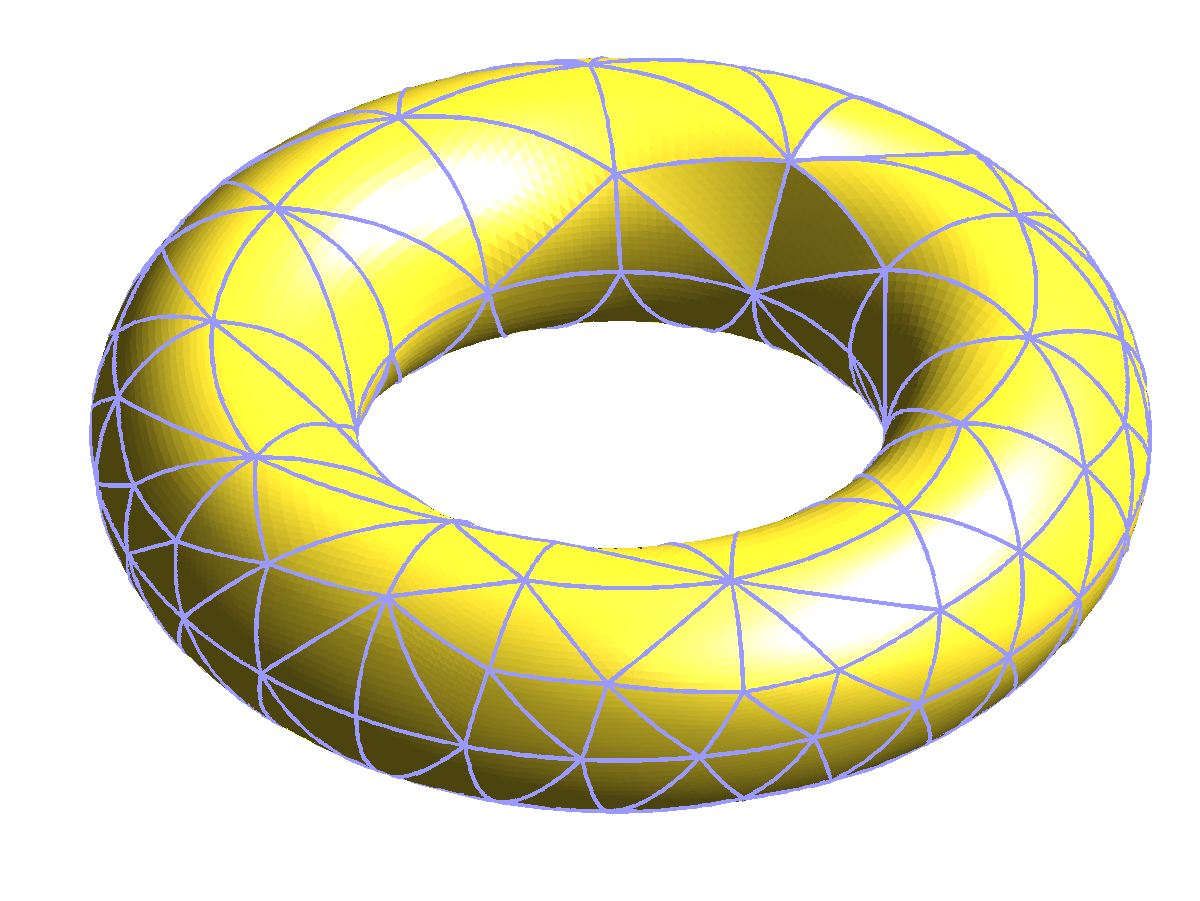
\includegraphics[width=6cm]{donut}}\htmlonly{\htmlimg{donut_small.png}{a donut}}\\
    you can notice that the mesh has a small default on some elements.
  \end{center}
\end{cmdexamples}
\begin{gfseealso}
  \kwl{gfplot}{gf\_plot}.
\end{gfseealso}
\newpage

%%%%%%%%%%%%%%%%%%%%%%% GF_PLOT_SLICE
\subsection{gf\_plot\_slice}
\begin{purpose}
\hypertarget{gfplotslice}
Plots a \slc\index{plotting slice}
\end{purpose}
\begin{synopsis}
@@[hfaces, htube, hquiver, hmesh]=gf_plot_slice(\tslc sl, \ldots)
@@\end{synopsis}
\begin{cmddescription}
  This function can be used to plot mesh slices. It is also used by
  the @@gf_plot_mesh@@ and @@gf_plot@@ functions.
  The various options are expected as a list pair ``option name''/``option value''.
  These options are:
\begin{center}
\begin{tabular}{|rlp{0.5\textwidth}|}
  \hline
  @@'data'@@           & @@[]@@     &   the data to be plotted (expected as a row vector or matrix such that @@size(D,2)==gf_slice_get(sl,'nbpts')@@).\\
  @@'mesh'@@           & @@'auto'@@ & @@'on'@@ $\to$ show the mesh (faces of edges), @@'off'@@ $\to$ ignore mesh.\\
  @@'mesh_edges'@@      & @@'on'@@   & show mesh edges ? (ignored if @@'mesh'@@ is off).\\
  @@'mesh_edges_color'@@   & @@[.6 .6 1]@@ & color (rgb or color name) of the mesh edges.\\
  @@'mesh_edges_width'@@   & @@.7@@     & width of mesh edges.\\
  @@'mesh_slice_edges'@@   & @@'on'@@   & also plot ``edges'' of the sliced part of the mesh ?\\
  @@'mesh_slice_edges_color'@@ & @@[.7 0 0]@@ & \\
  @@'mesh_slice_edges_width'@@ & @@.5@@ & \\
  @@'mesh_faces'@@      & @@'off'@@   & if @@'on'@@, fill the mesh faces (otherwise they are transparent).\\
  @@'mesh_faces_color'@@ & @@[.75 .75 .75]@@ & color of mesh faces (ignored if data is not empty).\\
  @@'pcolor'@@        & @@'on'@@     & if the data field is scalar, a color plot of its values is plotted.\\
  @@'quiver'@@        & @@'on'@@     & if the field is vector, represent arrows.\\
  @@'quiver_density'@@ & @@50@@       & density of arrows in quiver plot.\\
  @@'quiver_scale'@@   & @@1@@        & scaling of arrows in quiver plot.\\
  @@'tube'@@          & @@'on'@@     & use tube plot for 'filar' (1D) parts of the slice.\\
  @@'tube_color'@@     & @@'red'@@    & color of tubes (ignored if 'data' is not empty and 'pcolor' is on).\\
  @@'tube_radius'@@    & @@'0.5\%'@@   & tube radius; you can use a constant, or a percentage (of the mesh size) or a vector of nodal values (similar to the data field).\\
  @@'showoptions'@@  & @@'on'@@      & display the list of options before plotting.\\
    \hline
  \end{tabular}
\end{center}

On output, this function returns the handles to the various
graphical objects created: @@hmesh@@ is the handles to the mesh
lines, @@hfaces@@ is the handles to 2D faces created (patch objects), @@htube@@
is the handle of the tube plot (surface object), @@hquiver@@ is the handle obtained with the \mlab function @@quiver@@.
\end{cmddescription}

\begin{cmdexamples}
  \begin{center}
    \texonly{\includegraphics[width=.5\textwidth]{cuve3Dstreamlines}}\htmlonly{\htmlimg{cuve3Dstreamlinessmall.png}{streamlines of the fluid in a tank}}\\
  \end{center}

  Consider that you have a 3D \mf @@mf@@ and a vector field @@U@@ defined on this \mf, solution of the Stokes problem in a tank (see the demo \texttt{demo_stokes_3D_tank_draw.m} in the \texttt{tests} directory). 

  \begin{mcode}
figure;
% slice the mesh with two half spaces, and take the boundary of the resulting quarter-cylinder
sl=gf_slice(\{'boundary',\{'intersection',\{'planar',+1,[0;0;0],[0;1;0]\},\ldots
                                          \{'planar',+1,[0;0;0],[1;0;0]\}\}\},m,6);
Usl=gf_compute(pde.mf_u,U,'interpolate on', sl);  % interpolate the solution on the slice
% show the norm of the displacement on this slice
gf_plot_slice(sl,'mesh','on','data',sqrt(sum(Usl.^2,1)),'mesh_slice_edges','off');
  
% another slice: now we take the lower part of the mesh
sl=gf_slice(\{'boundary',\{'intersection',\{'planar',+1,[0;0;6],[0;0;-1]\},\ldots
                                        \{'planar',+1,[0;0;0],[0;1;0]\}\}\},m,6);
Usl=gf_compute(pde.mf_u,U,'interpolate on', sl);
hold on;
gf_plot_slice(sl,'mesh','on','data',sqrt(sum(Usl.^2,1)),'mesh_slice_edges','off');
  
% this slice contains the transparent mesh faces displayed on the picture
sl2=gf_slice(\{'boundary',\{'planar',+1,[0;0;0],[0;1;0]\}\},\ldots
            m,6,setdiff(all_faces',TOPfaces','rows')');
gf_plot_slice(sl2,'mesh_faces','off','mesh','on','pcolor','off'); 

% last step is to plot the streamlines
hh=[1 5 9 12.5 16 19.5]; % vertical position of the different starting points of the streamlines
H=[zeros(2,numel(hh));hh];

% compute the streamlines
tsl=gf_slice('streamlines',pde.mf_u,U,H);
Utsl=gf_compute(pde.mf_u,U,'interpolate on', tsl);

% render them with "tube plot"
[a,h]=gf_plot_slice(tsl,'mesh','off','tube_radius',.2,'tube_color','white'); 
hold off;
% use a nice colormap
caxis([0 .7]);
c=[0 0 1; 0 .5 1; 0 1 .5; 0 1 0; .5 1 0; 1 .5 0; 1 .4 0; 1 0 0; 1 .2 0; 1 .4 0; 1 .6 0; 1 .8 0];
colormap(c);
  \end{mcode}
\end{cmdexamples}
\begin{gfseealso}
  @@gf_slice@@
\end{gfseealso}
\newpage

\section{\gfm OO-commands}
\label{OOcommands}

The toolbox comes with a set of \Mlab
\WEB{http://www.mathworks.com/access/helpdesk/help/techdoc/matlab_prog/ch14_oop.shtml}{objects}
(look at the \texttt{@gf*} sub-directories in the toolbox directory).
These object are no more than the getfem object handles, which are
flagged by \mlab as objects.

In order to use these objects, you have to call their constructors: @@gfMesh@@,
@@gfMeshFem@@, @@gfGeoTrans@@, @@gfFem@@, @@gfInteg@@.  These constructor just
call the corresponding \gfm function (i.e.  @@gf_mesh@@, @@gf_mesh_fem@@, \ldots),
and convert the structure returned by these function into a \mlab object. There
is also a \texttt{gfObject}\index{gfObject}\hypertarget{gfObject} function which converts any getfem handle into the corresponding 
\mlab object.

With such object, the most interesting feature is that you do not have
to call the ``long'' functions names @@gf_mesh_fem_get(obj,\ldots)@@,
@@gf_slice_set(obj,\ldots)@@ etc., instead you just call the shorter
@@get(obj,\ldots)@@ or @@set(obj,\ldots)@@ whatever the type of @@obj@@ is.

A small number of ``pseudo-properties'' are also defined on these
objects, for example if @@m@@ is a @@gfMesh@@ object, you can use
directly @@m.nbpts@@ instead of @@get(m, 'nbpts')@@.

As an example, 
\begin{matlab}
% classical creation of a mesh object
>> m=gf_mesh('load', 'many_element.mesh_fem')
m =
     id: 2
    cid: 0
% conversion to a matlab object. the display function is overloaded for gfMesh.
>> mm=gfMesh(m)
gfMesh object ID=2 [11544 bytes], dim=3, nbpts=40, nbcvs=7
% direct creation of a gfMesh object. Arguments are the same than those of gf_mesh
>> m=gfMesh('load', 'many_element.mesh_fem')
gfMesh object ID=3 [11544 bytes], dim=3, nbpts=40, nbcvs=7
% get(m, 'pid_from_cvid') is redirected to gf_mesh_get(m,'pid from cvid')
>> get(m, 'pid_from_cvid', 3)
ans =
     8     9    11    15    17    16    18    10    12
% m.nbpts is directly translated into gf_mesh_get(m,'nbpts')   
>> m.nbpts
ans =
    40

>> mf=gfMeshFem('load','many_element.mesh_fem')
gfMeshFem object: ID=5 [1600 bytes], qdim=1, nbdof=99,
  linked gfMesh object: dim=3, nbpts=40, nbcvs=7
>> mf.mesh
gfMesh object ID=4 [11544 bytes], dim=3, nbpts=40, nbcvs=7
% accessing the linked mesh object
>> mf.mesh.nbpts
ans =
    40
>> get(mf.mesh, 'pid_from_cvid', 3)
ans =
     8     9    11    15    17    16    18    10    12
   
>> mf.nbdof
ans =
    99

% access to fem of convex 1
>> mf.fem(2)  
gfFem object ID=0 dim=2, target_dim=1, nbdof=9,[EQUIV, POLY, LAGR], est.degree=4
 -> FEM_QK(2,2)
>> mf.mesh.geotrans(1)
gfGeoTrans object ID= 0 dim=2, nbpts= 6 : GT_PK(2,2)
\end{matlab}

Although this interface seems more convenient, you must be aware that this
always induce a call to a mex-file, and additional \mlab code:
\begin{matlab}
>> tic; j=0; for i=1:1000, j=j+mf.nbdof; end; toc
elapsed_time =
    0.6060
>> tic; j=0; for i=1:1000, j=j+gf_mesh_fem_get(mf,'nbdof'); end; toc
elapsed_time =
    0.1698
>> tic; j=0;n=mf.nbdof;  for i=1:1000, j=j+n; end; toc                           
elapsed_time =
    0.0088
\end{matlab}

Hence you should always try to store data in \mlab arrays instead of repetitively
calling the getfem functions.


Avalaible object types are \hypertarget{gfCvStruct}gfCvStruct, 
\hypertarget{gfGeoTrans}gfGeoTrans, 
\hypertarget{gfEltm}gfEltm, 
\hypertarget{gfInteg}gfInteg, 
\hypertarget{gfFem}gfFem, 
\hypertarget{gfMesh}gfMesh, 
\hypertarget{gfMeshFem}gfMeshFem, 
\hypertarget{gfMeshIm}gfMeshIm, 
\hypertarget{gfMdBrick}gfMdBrick, 
\hypertarget{gfMdState}gfMdState, 
\hypertarget{gfModel}gfModel, 
\hypertarget{gfSpmat}gfSpmat, 
\hypertarget{gfPrecond}gfPrecond, 
\hypertarget{gfSlice}and gfSlice.


%\section{Various problems}
%\begin{itemize}
%\item ill conditioned system: check the eigenvalues on a small mesh. Check that the integration method is precise enough (or exact). Check your boundary conditions.
%\end{itemize}

\W \section*{Index}
%\htmlonly{\HlxSection{-5}{}*{\indexname}\label{gfmindex}}%
\texorhtml{\input{gfm.ind}}{\label{gfmindex}\htmlprintindex}
\end{document}
%endendend
